%%% The main file. It contains definitions of basic parameters and includes all other parts.

%% Settings for single-side (simplex) printing
% Margins: left 40mm, right 25mm, top and bottom 25mm
% (but beware, LaTeX adds 1in implicitly)
\documentclass[12pt,a4paper]{report}
\setlength\textwidth{145mm}
\setlength\textheight{247mm}
\setlength\oddsidemargin{15mm}
\setlength\evensidemargin{15mm}
\setlength\topmargin{0mm}
\setlength\headsep{0mm}
\setlength\headheight{0mm}
% \openright makes the following text appear on a right-hand page
\let\openright=\clearpage

%% Settings for two-sided (duplex) printing
% \documentclass[12pt,a4paper,twoside,openright]{report}
% \setlength\textwidth{145mm}
% \setlength\textheight{247mm}
% \setlength\oddsidemargin{14.2mm}
% \setlength\evensidemargin{0mm}
% \setlength\topmargin{0mm}
% \setlength\headsep{0mm}
% \setlength\headheight{0mm}
% \let\openright=\cleardoublepage

%% Generate PDF/A-2u
\usepackage[a-2u]{pdfx}

%% Character encoding: usually latin2, cp1250 or utf8:
\usepackage[utf8]{inputenc}

%% Prefer Latin Modern fonts
\usepackage{lmodern}

%% Further useful packages (included in most LaTeX distributions)
\usepackage{amsmath}        % extensions for typesetting of math
\usepackage{amsfonts}       % math fonts
\usepackage{amsthm}         % theorems, definitions, etc.
\usepackage{bbding}         % various symbols (squares, asterisks, scissors, ...)
\usepackage{bm}             % boldface symbols (\bm)
\usepackage{graphicx}       % embedding of pictures
\usepackage{fancyvrb}       % improved verbatim environment
\usepackage{natbib}         % citation style AUTHOR (YEAR), or AUTHOR [NUMBER]
\usepackage[nottoc]{tocbibind} % makes sure that bibliography and the lists
			    % of figures/tables are included in the table
			    % of contents
\usepackage{dcolumn}        % improved alignment of table columns
\usepackage{booktabs}       % improved horizontal lines in tables
\usepackage{paralist}       % improved enumerate and itemize
\usepackage[usenames]{xcolor}  % typesetting in color

%% Additional packages
\usepackage[allow-number-unit-breaks]{siunitx}
\usepackage{textcomp}

%% Algorithms (https://www.overleaf.com/learn/latex/algorithms)
\usepackage[linesnumbered,algoruled,boxed,lined]{algorithm2e}
\SetKwComment{Comment}{$\triangleright$\ }{}
\SetKwInOut{Parameter}{parameter}

%% Custom settings
\renewcommand\vec{\bm}

%%% Basic information on the thesis

% Thesis title in English (exactly as in the formal assignment)
\def\ThesisTitle{Trajectory planning for fast moving cars}

% Author of the thesis
\def\ThesisAuthor{Šimon Rozsíval}

% Year when the thesis is submitted
\def\YearSubmitted{2018}

% Name of the department or institute, where the work was officially assigned
% (according to the Organizational Structure of MFF UK in English,
% or a full name of a department outside MFF)
\def\Department{Department of Theoretical Computer Science and Mathematical Logic}

% Is it a department (katedra), or an institute (ústav)?
\def\DeptType{Department of Theoretical Computer Science and Mathematical Logic}

% Thesis supervisor: name, surname and titles
\def\Supervisor{Prof. RNDr. Roman Barták, Ph.D.}

% Supervisor's department (again according to Organizational structure of MFF)
\def\SupervisorsDepartment{Department of Theoretical Computer Science and Mathematical Logic}

% Study programme and specialization
\def\StudyProgramme{Computer Science}
\def\StudyBranch{Artificial Intelligence}

% An optional dedication: you can thank whomever you wish (your supervisor,
% consultant, a person who lent the software, etc.)
\def\Dedication{%
Dedication.
}

% Abstract (recommended length around 80-200 words; this is not a copy of your thesis assignment!)
\def\Abstract{%
Abstract.
}

% 3 to 5 keywords (recommended), each enclosed in curly braces
\def\Keywords{%
{key} {words}
}

%% The hyperref package for clickable links in PDF and also for storing
%% metadata to PDF (including the table of contents).
%% Most settings are pre-set by the pdfx package.
\hypersetup{unicode}
\hypersetup{breaklinks=true}

% Definitions of macros (see description inside)
%%% This file contains definitions of various useful macros and environments %%%
%%% Please add more macros here instead of cluttering other files with them. %%%

%%% Minor tweaks of style

% These macros employ a little dirty trick to convince LaTeX to typeset
% chapter headings sanely, without lots of empty space above them.
% Feel free to ignore.
\makeatletter
\def\@makechapterhead#1{
  {\parindent \z@ \raggedright \normalfont
   \Huge\bfseries \thechapter. #1
   \par\nobreak
   \vskip 20\p@
}}
\def\@makeschapterhead#1{
  {\parindent \z@ \raggedright \normalfont
   \Huge\bfseries #1
   \par\nobreak
   \vskip 20\p@
}}
\makeatother

% This macro defines a chapter, which is not numbered, but is included
% in the table of contents.
\def\chapwithtoc#1{
\chapter*{#1}
\addcontentsline{toc}{chapter}{#1}
}

%% Draw black "slugs" whenever a line overflows, so that we can spot it easily.
%\overfullrule=1mm

%%% Macros for definitions, theorems, claims, examples, ... (requires amsthm package)

\theoremstyle{plain}
\newtheorem{thm}{Theorem}
\newtheorem{lemma}[thm]{Lemma}
\newtheorem{claim}[thm]{Claim}

\theoremstyle{plain}
\newtheorem{defn}{Definition}

\theoremstyle{remark}
\newtheorem*{cor}{Corollary}
\newtheorem*{rem}{Remark}
\newtheorem*{example}{Example}

%%% An environment for proofs

%%% FIXME %%% \newenvironment{proof}{
%%% FIXME %%%   \par\medskip\noindent
%%% FIXME %%%   \textit{Proof}.
%%% FIXME %%% }{
%%% FIXME %%% \newline
%%% FIXME %%% \rightline{$\square$}  % or \SquareCastShadowBottomRight from bbding package
%%% FIXME %%% }

%%% An environment for typesetting of program code and input/output
%%% of programs. (Requires the fancyvrb package -- fancy verbatim.)

\DefineVerbatimEnvironment{code}{Verbatim}{fontsize=\small, frame=single}

%%% The field of all real and natural numbers
\newcommand{\R}{\mathbb{R}}
\newcommand{\N}{\mathbb{N}}

%%% Useful operators for statistics and probability
\DeclareMathOperator{\pr}{\textsf{P}}
\DeclareMathOperator{\E}{\textsf{E}\,}
\DeclareMathOperator{\var}{\textrm{var}}
\DeclareMathOperator{\sd}{\textrm{sd}}

%%% Transposition of a vector/matrix
\newcommand{\T}[1]{#1^\top}

%%% Various math goodies
\newcommand{\goto}{\rightarrow}
\newcommand{\gotop}{\stackrel{P}{\longrightarrow}}
\newcommand{\maon}[1]{o(n^{#1})}
\newcommand{\abs}[1]{\left|{#1}\right|}
\newcommand{\dint}{\int_0^\tau\!\!\int_0^\tau}
\newcommand{\isqr}[1]{\frac{1}{\sqrt{#1}}}

%%% Various table goodies
\newcommand{\pulrad}[1]{\raisebox{1.5ex}[0pt]{#1}}
\newcommand{\mc}[1]{\multicolumn{1}{c}{#1}}


% Title page and various mandatory informational pages
\begin{document}
%%% Title page of the thesis and other mandatory pages

%%% Title page of the thesis

\pagestyle{empty}
\hypersetup{pageanchor=false}
\begin{center}

\centerline{\mbox{
\includegraphics[width=166mm]{../img/logo-en.pdf}}}

\vspace{-8mm}
\vfill

{\bf\Large MASTER THESIS}

\vfill

{\LARGE\ThesisAuthor}

\vspace{15mm}

{\LARGE\bfseries\ThesisTitle}

\vfill

\Department

\vfill

\begin{tabular}{rl}

Supervisor of the master thesis: & \Supervisor \\
\noalign{\vspace{2mm}}
Study programme: & \StudyProgramme \\
\noalign{\vspace{2mm}}
Study branch: & \StudyBranch \\
\end{tabular}

\vfill

% Zde doplňte rok
Prague \YearSubmitted

\end{center}

\newpage

%%% Here should be a bound sheet included -- a signed copy of the "master
%%% thesis assignment". This assignment is NOT a part of the electronic
%%% version of the thesis. DO NOT SCAN.

%%% A page with a solemn declaration to the master thesis

\openright
\hypersetup{pageanchor=true}
\pagestyle{plain}
\pagenumbering{roman}
\vglue 0pt plus 1fill

\noindent
I declare that I carried out this master thesis independently, and only with the cited
sources, literature and other professional sources.

\medskip\noindent
I understand that my work relates to the rights and obligations under the Act No.~121/2000 Sb.,
the Copyright Act, as amended, in particular the fact that the Charles
University has the right to conclude a license agreement on the use of this
work as a school work pursuant to Section 60 subsection 1 of the Copyright Act.

\vspace{10mm}

\hbox{\hbox to 0.5\hsize{%
In ........ date ............	% FIXME!
\hss}\hbox to 0.5\hsize{%
signature of the author
\hss}}

\vspace{20mm}
\newpage

%%% Dedication

%\openright

%\noindent
%\Dedication

%\newpage

%%% Mandatory information page of the thesis

\openright

\vbox to 0.5\vsize{
\setlength\parindent{0mm}
\setlength\parskip{5mm}

Title:
\ThesisTitle

Author:
\ThesisAuthor

\DeptType:
\Department

Supervisor:
\Supervisor, \SupervisorsDepartment

Abstract:
\Abstract

Keywords:
\Keywords

\vss}

\newpage

\openright
\pagestyle{plain}
\pagenumbering{arabic}
\setcounter{page}{1}


%%% A page with automatically generated table of contents of the master thesis

\tableofcontents

%%% Each chapter is kept in a separate file
\chapter*{Introduction}
\addcontentsline{toc}{chapter}{Introduction}

Autonomous vehicles are slowly but steadily making their way from research facilities to the public roads around the world and it seems inevitable that they will soon become part of our daily lives. Autonomous vehicles could have a significant impact on transportation of people and goods. For example, thousands of people die in car accidents every year because of human error \cite{Road_accidents}. Some believe that replacing humans with accurate electronic sensors and computer algorithms, which never make errors, could reduce the number of accidents on roads significantly. It seems that companies around the world see the potential in this technology and invest a lot of effort and money in research of self-driving cars. Even though nobody can guarantee that autonomous vehicles will never make errors and that they will solve other problems of road transportation we face today, the trend is clear. The key to the success of this technology will be reliable and robust algorithms which will work in all driving scenarios and weather conditions and which the public will trust.

The idea of self-driving cars is far from new. Prototypes of autonomous vehicles were demonstrated on public roads as early as the 1980s. Among some of the well-known projects from this era were for example the NavLab vehicle of the Carnegie Mellon University \cite{NavLab} or the project of Ernst Dickmanns in cooperation with the Daimler company \cite{Ernst_Dickmanns}. The DARPA challenges, organized between 2004 and 2007, gained a lot of media attention. We can see that self-driving cars are no longer just science fiction. Since then, many driving assistants such as adaptive cruise control, lane keeping assistants, parallel parking assistants, collision warning, and emergency braking assistants started appearing in commercially available vehicles. Some systems, like the Tesla Autopilot, go even further and allow complex autonomous maneuvers such as overtaking other vehicles.

These commercially available assistants provide the user only with partial autonomy. The driver is required to pay attention to the road all the time and he or she is required to be prepared to take control of the vehicle if the system fails or if it cannot handle the traffic situation. Fully autonomous vehicles will not require any human interaction. They might even lack any means of manual driving. The computer will be responsible for the vehicle from the start to the destination irrespective of the weather or traffic. There is an ongoing research into full autonomy by some companies like Waymo and Uber and prototypes of vehicles equipped with this technology are already being tested on public roads.

One of the key problems in autonomous driving is the ability to find a good trajectory for the car in various different scenarios. This trajectory must be safe for the passengers of the vehicle and for other road users. It must also conform to road limitations such as speed limits and other traffic rules. Automated planning is an area of artificial intelligence which gives us means to formulate and solve this problem. For a well-defined planning problem which describes the physics of the vehicle and our goals, we can find a sequence of control inputs which will drive the vehicle to the goal as we need.

In this thesis, our focus is trajectory planning for fast moving cars. We will design and develop an autonomous vehicle for the task of autonomous racing. The racing scenario is simplification of real-world driving. It requires us to avoid collisions and to find efficient trajectories while moving at high speeds and to adapt to unforeseen obstacles on the road. At the same time, this simplified problem allows us to ignore any traffic rules. We do not have to consider any speed limits, crossroads, stop signs, or other road users.

We will create an autonomous racing agent which utilizes a trajectory planning algorithm to find fast routes along the racing circuit. We will test different algorithms for searching solutions to the planning problem and compare them in a series of experiments on a real-world car model with sensors and an embedded on-board computer.

First, we introduce the autonomous driving problem and split it into several sub-problems. We give a brief overview of related works in the field of autonomous driving. We describe an architecture of an artificial agent for the task of autonomous racing.

Next, we examine the individual sub-problems we must solve in order to create the racing agent. We analyze and formulate the trajectory planning problem for a fast moving car. We describe adaptations of several planning algorithms for our specific problem. We study how the vehicle reacts to steering commands and we describe a model of the actuators and of the vehicle movement. We then describe algorithms for following of a the planned trajectory.

Finally, we implement the racing agent and we conduct several experiments to verify the performance and success rate of our algorithms and we test them on a custom-built real-world experimental vehicle.

\chapter{Autonomous Driving Background}

Autonomous driving is a complex task. The vehicle collects information about the surrounding environment from its sensors and then it decides its next control input to the actuators of the vehicle. There are two general approaches to this problem: end-to-end driving and decomposition into several subproblems.

The end-to-end driving approach takes the sensor data as an input and maps them to the control inputs. The end-to-end driving algorithm can be implemented for example using a stream of images form a front-facing camera and a neural network trained using supervised or reinforcement learning. It was successfully demonstrated for example in ALVINN, a simple 3-layer neutral network used in the NavLab autonomous vehicle of Carnegie Mellon University in 1989 \cite{ALVINN}, or more recently with a deep convolutional neural network by Nvidia \cite{Nvidia}. End-to-end driving avoids explicit modeling of the world and the vehicle and it relies on the knowledge extracted from the training data or by learning by trial and error during reinforcement learning.

The other approach is to split the complex problem into several smaller problems, which are solved independently. We can split the problem into three main subproblems: Perception, Planning, and Control.

Perception is the process of collecting data from the sensors and processing them to obtain the current state of the world and the internal properties of the vehicle. The task of determining the position of the vehicle on a map is called localization. The sensors which would be used for localization are cameras, radars, ultrasonic sensors, and LIDARs. The data from these sensors can be used to determine distances to nearby obstacles in different directions. Based on the previous known position of the vehicle, the estimate of its movement, and the distances to obstacles in different directions, the position on a known map can be determined using an algorithm such as Adaptive Monte Carlo Localization (AMCL) \cite{AMCL_position_estimation} \cite{AMCL_adaptive_sampling}. In certain scenarios, the relative distances to the obstacles might not be enough to determine correct position. This can happen for example when the vehicle is driving through a straight tunnel and the distances to the walls are constant even though the vehicle is moving. It is useful to combine readings from multiple sensors which provide odometry such as wheel encoders which measure how many times the wheels turn and an intrinsic measurement unit (IMU) with gyroscopes and accelerometers which measures the linear and angular acceleration of the vehicle. The combination of multiple different types of sensors is called sensor fusion. Kalman filter is an example of an algorithm which is frequently used to fuse data from different sources \cite{Kalman_filter}.

The vehicle must also be able to read road signs and road surface markings for driving along public roads. The data from the sensors can also be used to detect obstacles and for obstacle tracking. The type of obstacle is then identified and in the case of dynamic obstacles such as other cars, bicyclists, pedestrians, animals, or moving inanimate objects their movement in time must be predicted to prevent collisions.

The geometry of a car-like vehicle limits its controllability. The vehicle cannot turn while it is stopped and it can only start turning once it is moving forwards or backwards. Usually the only way to control the turning radius is by turning the front wheels and the rear wheels are fixed. In order to be able to make any reasoning about the future states of the vehicle, we must be able to predict the effect of a sequence of control inputs on the motion of the vehicle. Without an accurate model of the vehicle we could select a trajectory which cannot be safely followed, or which would be ineffective. We will discuss vehicle modelling in detail in chapter Vehicle Model.

With the knowledge of the vehicle model, we can search for a plan consisting of control inputs over some time period which will result in a collision-free trajectory through the environment which minimizes some cost function (e.g., the time it will take to reach some goal location). Planning several steps into the future can give us an advantage over a simple end-to-end driving approach. For example, in the case of autonomous racing, the agent can take advantage of the knowledge of the racing track map, and account for the shape of the track hidden around the next corner. We should be able to decide, when to slow down and when to accelerate, as well as at which point to start turning into a corner, in order to reach the best lap times. We call this subproblem trajectory planning.

Executing the sequence of control inputs one by one might cause the vehicle to drive off the track. The trajectory planning algorithm relies on a vehicle model which might not be accurate. The reference trajectory is therefore idealized, and it might not be possible to achieve it exactly by the actual vehicle. It might also lead to a collision with an obstacle on the track which was not known at the time of planning. A trajectory following algorithm chooses the next action based on the current state of the vehicle and the distance to the position, vehicle orientation, and speed at a corresponding point on the reference trajectory. The algorithm should also avoid any unexpected obstacles detected by the sensors.

The actual effects of the control inputs are measured by the sensors and the control algorithm tries to minimize the error between the planned trajectory and the actual trajectory of the vehicle in its next step. This process is referred to in control theory as closed feedback loop.

\section{Requirements}

In this thesis, we will design and develop an autonomous vehicle for the task of autonomous racing. The racing scenario is a simplification of real-world driving. It requires us to avoid collisions and to find efficient trajectories while moving at high speeds and to adapt to unforeseen obstacles on the road. At the same time, this relaxed problem allows us to ignore any traffic rules. We do not have to consider any speed limits, crossroads, or stop signs.

This problem is inspired by the F1/10 competition organized by the University of Pennsylvania and the University of Virginia \cite{F1/10_web}. We will use the resources from this competition to build a similar autonomous vehicle based on an RC car. To evaluate the performance of the vehicle, we will use the criteria of Time Trial Race of F1/10. In the Time Trial Race, the vehicle drives for 5 minutes around a circuit trying to achieve as many laps as possible without a collision with the boundary of the track or with static obstacles on the track. The time of the fastest lap is also recorded.

We will create an autonomous racing agent which utilizes a trajectory planning algorithm to find fast routes along the racing circuit. We will test different algorithms for searching solutions to the planning problem and compare them in a series of experiments on a real-world car model with sensors and an embedded on-board computer.

\section{Related Work}

In this section we will go through several interesting approaches to path and trajectory planning from the area of robotics and autonomous cars.

Shakey the Robot was a project at the Stanford Research Institute in the 1960s. For the purposes of efficient route finding the A* algorithm was designed by Nils J. Nilsson and his coworkers \cite{Nilsson}. This algorithm is widely used for solving various graph search problems thanks to its simplicity, completeness, and optimality. The NavLab autonomous vans of the Carnegie Mellon university was one of the first autonomous vehicles tested on public roads in the 1980s and 1990s. One of the interesting results of their work is the Pure Pursuit control algorithm \cite{Pure_pursuit}.

Steven M. LaValle designed a randomized path planning algorithm for vehicles with kinodynamic driving constraints and high-dimensional configuration spaces called Rapidly-Exploring Random Trees (RRT) \cite{RRT}. This algorithm randomly samples the configuration space and steers the vehicle towards the sampled point in the space. A tree of feasible paths in the configuration space rooted in the starting position is constructed until a path which ends in the goal position is found. The algorithm is probabilistically complete, but it is not optimal. The algorithm was extended by many times in order to converge faster and to be optimal. The optimal variant of the algorithm, RRT* \cite{RRT_star}, is unfortunately hard to use for car-like vehicles.

In 2007, the DARPA Urban Challenge took place in the USA which was successfully completed by several vehicles with different approaches to trajectory planning. The entry from the Carnegie Mellon University, Boss, won the competition. It uses the Anytime D* algorithm for navigation in unstructured environment \cite{Boss}. The Stanford team used an algorithm called Hybrid A* in their vehicle called Junior \cite{Junior}. This algorithm is an extension of the A* algorithm which discretizes the continuous search space into a discrete grid to avoid examining similar configurations multiple times, but it keeps the information about the trajectories in the continuous configuration space to produce smooth feasible trajectories. The team from MIT used modified RRT algorithm in their vehicle \cite{RRT_urban_driving}.

\chapter{Artificial Racing Agent}
\label{chapter:agent}

In this chapter we will first analyze how human racing drivers approach the task of car racing. We will then use this information to design a behavior of an autonomous agent and decompose the problem into several smaller tasks. We will discuss how we can analyze the racing track and prepare it for trajectory planning.

\section{Racing Line}
\label{sec:racing_line}

When a human driver drives on a racing circuit, his or her task is to complete several laps around the circuit in a time period as short as possible. In order to minimize the lap times, the driver trades off the total distance the car travels for the average speed at which it moves. The trajectory of the vehicle through the racing track is sometimes referred to as the racing line and it depends on the shape of the track and on the vehicle. The driver will follow different racing lines for different vehicles on the same circuit based on many their different properties such as maximum speeds, acceleration, braking power, or the grip of the tires.

For a turn with a steady curvature there is a maximum speed at which a specific car can go and stay on the track. Exceeding this speed will cause a loss of friction between the tires and the road surface and the tires will not be able to exert enough lateral force to keep the car on the curve and the car will start to travel along a curve with a greater radius than the one commanded by the driver. This situation is called understeer or oversteer, depending on whether it was the front or rear wheels which lost the friction and which wheels are powered by the engine.

\begin{figure}
	\label{fig:oversteer_understeer}
	\missingfigure{Understeer vs. oversteer}
	\caption{This figure shows the difference between oversteer and understeer.}
\end{figure}

On the other hand, for a constant vehicle speed, the vehicle can safely travel along any curve with a radius greater than the minimum safe radius. The driver will therefore try to follow curves with higher radii when going through corners but only to the point where the maximum safe speed reaches the maximum speed of the vehicle. Increasing the curvature when it is not possible to increase the speed adds to the distance the car travels but it does not increase the average speed and therefore leads to a higher lap time.

The trajectory of the vehicle as it goes through a corner can be split into several stages. First, the vehicle aligns itself to the outer edge of the track. Second, the vehicle must adjust its speed so it can safely stay on the curve. It is common to use the brakes mostly while the vehicle is moving straight to avoid locking the wheels in mid-turn. Third, the car starts turning at a turn-in point to go through the apex of the curve at the desired moment. Fourth, the vehicle goes through an apex, which is the point, where it is the closest to the inner edge of the track. Next, the vehicle starts exiting the corner and enters another part of the track.

There are two common ways of going through a corner, a classical one and one called late apex. The classical way of leaving the corner is to keep the constant curvature of the turn and to align the vehicle with the outer edge of the track. The late apex is achieved by starting to turn into the corner later and exiting the corner much closer to the inner edge of the track than the classical way. During the late apex turn, the vehicle slows down more before entering the corner and it straightens the line before hitting the apex allowing for greater exit speed. The comparison between these two lines can be seen in Figure~\ref{fig:apex}.

\begin{figure}
	\label{fig:apex}
	\missingfigure{Classical line and Late apex: https://drivingfast.net/racing-line}
	\caption{Classical line vs. Late apex}
\end{figure}

Another factor which affects the speed at which the driver can go through a corner is the shape of the track around the corner. When there is a straight stretch following the corner, the driver can maximize the speed at which the vehicle leaves the corner to increase the average speed. If there is another corner immediately after the first one, the driver must plan ahead and adjust the speed before entering the first corner to a level at which the exit speed of the first corner will be appropriate to go through the following corner.

From the description of the racing behavior of human expert drivers, it is apparent that the key components of choosing the optimal racing line are the knowledge of the behavior of the vehicle and the shape of the track. The knowledge of the track gives the driver an opportunity to plan how he or she is going to approach driving on the track. The driver can plan how to approach each individual corner and what speeds and turning radii are optimal and still safe.

\section{Artificial Agent}

\begin{defn}\label{def:rational_agent}
    A rational agent is an entity which gathers information from the environment through sensors and changes the state of the environment in order to maximize some performance measure.
\end{defn}

A racing driver can be thought of as a rational agent as defined in definition~\ref{def:rational_agent}. The driver observes the position of the vehicle on the racing track and the state of the vehicle as it moves along the track. He also observes the distance to the boundaries of the track and to any obstacles which can be present on the track. The driver reacts to these perceptions by giving control inputs to the vehicle through the steering wheel, brake and accelerator pedals, and shifting into different gears. The performance measure is the lack of collisions with the boundaries of the track or any obstacles on the track and minimizing of the lap time.

An artificial racing agent would use electronic sensors such a LIDAR, wheel encoders, an \gls{IMU}, or a camera to observe the state of the environment. Based on this observation, the agent can estimate its state in the world and the state of other entities in the world, such as obstacles or opponents. Based on this information, the agent has to select a control input for the actuators of the vehicle.

The agent can use the information about its initial state and calculate a time-optimal racing line from this initial state through the whole circuit up to the finish line using a trajectory planning algorithm. Depending on the size of the circuit, this could be a computationally expensive operation. If later on there is a need to re-plan the trajectory during the race, because the vehicle could not follow the trajectory accurately and it is necessary to come up with a contingency plan, the vehicle might have to repeat the expensive calculation. Instead, the agent can analyze the shape of the circuit and identify the corners and focus its effort only on the next two or three corners ahead of him.

\subsection{Decision Process}

An agent is sometimes described in the form of an agent function. This function takes the data from the sensors and outputs a command for the actuators. The command is then executed and it has an effect on the environment. In the next step we measure the changed state of the environment and the agent reacts to this changed state. The agent can select the next command in an order to correct the outcome of the previous command when it is different from the predicted outcome. This process is then repeated over and over in a so-called closed-feedback loop.

In order to avoid describing the logic of the racing agent in a single complicated function, we can divide the decision process of the agent into several smaller independent sub-problems: localization, track analysis and waypoint selection, trajectory planning, and trajectory following. Some of these sub-problems output information which is necessary as an input for another of these sub-problems they form nodes of a dependency graph of the decision process which is visualized in Figure~\ref{fig:racing_agent_diagram}.

There is one more reason to decompose the task into several sub-problems. The rate at which the individual sub-problems produce outputs is different and they work asynchronously. While the trajectory following algorithm should react to any location update with an action to correct the movement of the vehicle and it should do this many times per second, the planning process of a trajectory will take some non-trivial time and so the trajectory planning process will have much lower output frequency.

\begin{figure}[]\centering
	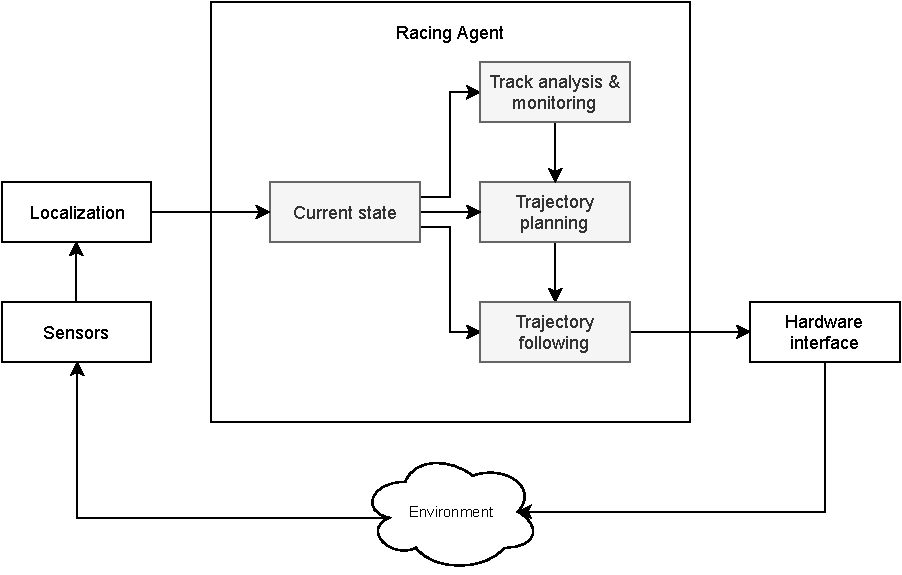
\includegraphics[width=125mm]{../img/racing_agent_diagram.pdf}
	\caption{A diagram of the decision process of the racing agent.}
	\label{fig:racing_agent_diagram}
\end{figure}

\paragraph{Current state} As the vehicle moves on the track, the agent needs to know its current state: its position on the map, orientation, and speed. A localization algorithm collects the data from different sensors and estimates the current state of the vehicle. The accuracy and the frequency of state updates depend greatly on the capabilities of the sensors and the processing power of the on-board computer. The agent takes the raw data from a localization algorithm and produces a convenient representation of the current state for track monitoring, trajectory planning, and trajectory following.

\paragraph{Track analysis \& monitoring} Before the race begins, the agent analyses the track and finds the corners and bends on the track and marks a coordinate of a point near the apex of the corner and forms a list of waypoints along the track. During the race, the agent will keep track of which of the waypoints discovered during track analysis it drove past the last. The waypoint selection process will publish the following $n$ waypoints as the next goal for trajectory planning. The parameter $n\in\mathbb{N}$ is the lookahead of the agent. The selection of this parameter is a trade off between the quality of the trajectory and the size of the configuration space that will be searched. This directly affects the update rate of the trajectory planning process.

\paragraph{Trajectory planning} The trajectory planning algorithm finds a feasible trajectory from the last state of the vehicle estimated by the localization algorithm through the selected waypoints. The trajectory planning process will start planning a new trajectory as soon as it finishes planning the previous one. As the agent drives along the circuit and drives past a waypoint, the trajectory planning algorithm receives a new sequence of waypoints and the next trajectory it plans will account also for the next corner of the circuit within the lookahead instance. Planning can be a slow process even when we try to reduce the size of the search space as much as possible. For the practical application, the planning algorithm must update the trajectories faster than the vehicle moves through the circuit. If the agent comes to the end of an old reference trajectory and it has no update, it has to stop and wait for an update. This would obviously affect the lap time which is undesirable.

\paragraph{Trajectory following} The latest reference trajectory and the current estimate of the state of the vehicle is used to calculate the next command for the actuators of the vehicle. In the ideal case, this trajectory following algorithm will send the commands to the hardware at the maximum possible rate which the hardware is capable of. In practice we are limited by the rate at which we receive the state estimates from the localization algorithm. The trajectory following algorithm is also responsible for collision avoidance either by actively guiding the vehicle around the obstacles it might hit, or by slowing down the vehicle while waiting for a new reference trajectory.


\chapter{Trajectory Planning}

The main focus of this thesis is the problem of trajectory planning for a fast moving car. In this chapter, we will analyze this problem in depth. We will first look into the planning problem in general and then we will discuss what the term ``fast moving cars'' means and how trajectory planning for a fast car is different from the general planing problem.

With the knowledge of the theory, we will formulate our trajectory planning problem. We will consider several well-known search algorithms used to solve planning problems and adapt them to our problem.

The solution of the planning problem will be a trajectory. A trajectory is the description of both a path the vehicle should follow and also a speed profile. If a robot is able to follow this trajectory, it will have an advantage over reactive steering algorithms, such as end-to-end driving, as it will be able to go through a series of corners efficiently by slowing down and accelerating at convenient times and by following an appropriate racing line. We will discuss a way of following the trajectory later in Chapter~\ref{chapter:following}.

\section{Introduction to Planning}

In this section, we will give a brief overview of the basic concepts of automatic planning and planning under differential constraints. The main source of the information for this chapter is a book by Steven M. LaValle called \textit{Planning Algorithms} \cite{lavalle_2006}. This book describes all of the topics in this section in much more detail and it is a good source of further information on this topic.

\subsection{Automatic Planning}

Planning is the task of solving some problem by finding a sequence of actions, which transforms the world to some desired state. The world of a planning problem is defined in terms of states and actions.

A single state is a full description of all of the important aspects of the world. A state can be encoded in many different ways, for example it can be a set of logical propositions which hold true in the given state or a vector of an $n$-dimensional vector of real numbers. All of the possible states of the world form a state space.

An action is a way of changing a state of the world into a different state. Not all actions can be applied in all states and so the set of possible actions can differ from state to state. All of the actions together then form an action space.

The planning task is to find a sequence of actions, which changes the state of the world from a given initial state to some desired state. Such sequence of actions is referred to as a feasible plan.

With the intuition of what a planning problem is, we can formulate it formally:

\begin{defn}[Planning Problem]
	\label{def:basic_planning_problem}
	A planning problem is a tuple $\left(X, U, f, x_0, g\right)$ consisting of:
	
	\begin{enumerate}
		\item A \textit{nonempty set} $X$ of world states, called the \textit{state space}.
		\item For each state $x\in X$, a set of actions $U(x)$.  A set of all actions $U=\bigcup\limits_{x\in X} U(x)$ is called an \textit{action space}.
		\item A \textit{state transition function} $f$ defined for every $x\in X$ and $u\in U(x)$, which produces the state of the world after applying the action $u$ to the state $x$.
		\item An \textit{initial state} of the world $x_0\in X$.
		\item A goal region $X_g\subset X$.
	\end{enumerate}
\end{defn}

\begin{defn}[Feasible Plan]
	A solution to a planning problem $\left(X, U, f, x_0, g\right)$ is a \textit{feasible plan}, which a finite sequence of actions $\langle u_0, u_1, \ldots, u_k\rangle\in U^*$ such that:	
	\begin{gather*}
		\forall i \in \left\{0,1,\ldots,k\right\}: u_i\in U(x_i) \wedge x_{i+1}=f(x_i, u_i) \\
		x_{k+1} \in X_g.
	\end{gather*}
\end{defn}

\begin{defn}[Optimal Plan]
	Let $\left(X, U, f, x_0, g\right)$ be a planning problem and $\Pi=\left\{\pi\in U^* \mid \pi \text{ is a feasible plan}\right\}$ a set of all feasible plans. We say that a plan $\pi^*\in \Pi$ is an optimal plan with respect to a cost function $\gamma: \Pi \rightarrow \mathbb{R}$ if
	
	\[
		\pi^*=\argmin_{\pi\in\Pi} \gamma(\pi).
	\]
\end{defn}

\subsubsection{Reachability Graph}

We can imagine that the states form vertices of a graph $G=(V, E)$ and the applications of actions through the state transition function form directed edges between the vertices:

\begin{equation*}
\begin{aligned}
	V&=X \\
	E&=\left\{(x_1, x_2) \mid \exists u \in U(x_1): x_2 = f(x_1, u) \right\}.
\end{aligned}
\end{equation*}

This graph can in general have several subgraphs. We are only interested in the component, which contains the initial $x_0$ and all the vertices which are reachable from $x_0$ via a directed path. A feasible plan is then a directed path in the graph starting in the initial state vertex $x_0$ and ending in any of the goal states vertices. Finding a path in a graph is well-studied problem and there are several efficient algorithms to solve it, such as the Dijkstra algorithm or its extension called A*.

The size of the state space and the action spaces has great impact on the way how we approach the planning problem and how we find a solution. If the graph is finite or if the the number of vertices is countably infinite and the branching factor is finite, we can find the solution (if one exists) with a systematic search algorithm in a finite amount of time. If no solution exists and the graph is infinite, the algorithm will be trying different plans infinitely. In practice this can be avoided with a limiting criterion, such as maximum length of a plan.

When the number of vertices is uncountably infinite or the branching factor is infinite, the problem becomes much harder and we cannot rely on a simple graph search anymore. We will soon see, that the state space of all of the vehicle configurations in our problem is uncountably infinite. These problems can be solved using \textit{sampling algorithms}.

We must keep in mind that the number of states of the system can be very high even if it is finite because the state space represents all of the combinations of the state variables of the world.

\subsection{Planning Under Differential Constraints}
\label{sec:planning_under_differential_constraints}

When describing the motion of a car-like robot on a two-dimensional plane, we assume that we can treat it as a rigid body, usually represented as a bounding rectangle. The configuration of the rigid body is then described by the pose of the vehicle: the $\left(x,y\right)$ Cartesian coordinates of a fixed reference point of the body in the world reference frame, and the heading angle $\theta$ between the longitudinal axis of the vehicle and the $x$ axis of the world reference frame. The $(x, y)$ location is in some bounded area $P\subset\mathbb{R}^2$ and the heading angle is an arbitrary angle $\theta\in\left[0,2\pi\right)$. This simple configuration space already has three continuous dimensions and it is uncountably infinite.

The kinematics and dynamics of a robots are typically described by differential equations. These equations give us the velocities at which the state of the robot changes when an action is applied. As an example of these constraints, we can look at a model of a \textit{simple car} \cite[Section~13.1.2.1]{lavalle_2006}.

\begin{example}
The state space of a simple car will consist of the poses in an infinite 2D plane $(x, y, \theta)$ as we described it earlier. The control inputs are two dimensional vectors $\left(u_s, u_\varphi\right)$, where $u_s$ is the commanded speed of the vehicle in the direction perpendicular to the rear axis, and $u_\varphi$ is the steering angle of the front wheels. For a better understanding of this example, see the Figure~\ref{fig:simple_car}.

For a car with a wheelbase length $L\in\mathbb{R}$, its velocity can be approximated by this set of equations:

\begin{equation}
\begin{aligned}
	\dot{x}&=u_s \cos \theta \\
	\dot{y}&=u_s \sin \theta \\
	\dot{\theta}&=\dfrac{u_s}{L} \tan u_\varphi.
\end{aligned}
\end{equation}
\end{example}

\begin{figure}
	\centering
	\label{fig:simple_car}
	
	\begin{tikzpicture}[
		axis/.style={thin, densely dashed, gray}
	]
	
	% the axes
	\path[name path=AX] (-1,0)--(8,0);
	\draw[thick, ->] (-1,0)--(8,0) node[right]{$x$};
	\draw[thick, ->] (0,-1)--(0,6.5) node[above]{$y$};
	
	\def\stateTheta{45} % heading angle of the vehicle
	\def\statePhi{-24} % steering angle of the front wheels
	\def\L{2.5} % wheelbase of the vehicle
	\def\W{1.45} % axle width
	\def\w{2} % width of the vehicle
	\def\l{4.5} % length of the vehicle
	\def\wW{0.2} % wheel width
	\def\wL{0.5} % wheel length
	\def\xoffset{3cm}
	\def\yoffset{0.8cm}
	
	% the rotated vehicle
	\begin{scope}[xshift=\xoffset, yshift=\yoffset]
	\begin{scope}[rotate=\stateTheta]
    
   		% longitudinal axis
   		\path[name path=AL] (-2.5, \w/2) -- (\l+2, \w/2);
   		\draw[axis] (-2.5, \w/2) -- (\l+2, \w/2);

		% visualize theta
		\path [name intersections={of=AL and AX, by={X}}];
		\draw[rotate=-\stateTheta] (X)++(0.7,0) arc (0:\stateTheta:0.7) node[right, yshift=-1mm, xshift=1mm] {$\theta$}; % theta
    
    	% shape of the vehicle
		\draw (0, 0) rectangle (\l, \w);		
		
		% axle coordinates
		\def\rearX{\l/2 - \L/2}
		\def\frontX{\l/2 + \L/2}
		\def\rightY{\w/2 - \W/2}
		\def\leftY{\w/2 + \W/2}
		
		\coordinate (front) at (\frontX, \w/2);
		\coordinate (rearLeft) at (\rearX, \w/2 + \W/2);
		\coordinate (frontLeft) at (\frontX, \w/2 + \W/2);
		
		% visualize the wheelbase length		
		\draw[axis] (rearLeft) -- ++(0, 1);
		\draw[axis] (frontLeft) -- ++(0, 1);		
		\draw[<->, >=latex] ($ (rearLeft) + (0, 0.8) $) -- node[above, xshift=-1.5mm, yshift=-1mm] {$L$} ($ (frontLeft) + (0, 0.8) $);
		
		\draw[thick] (\rearX - \wL/2, \rightY - \wW/2) rectangle (\rearX + \wL/2, \rightY + \wW/2); % rear right wheel/tire
		\draw[thick] (\rearX - \wL/2, \leftY - \wW/2) rectangle (\rearX + \wL/2, \leftY + \wW/2); % rear left wheel/tire
		\filldraw[thick] (\rearX, \rightY + \wW/2) -- (\rearX, \w/2) circle (2pt) node[right, xshift=1mm] {$(x, y)$} -- (\rearX, \leftY - \wW/2); % the axle 
		
		% front axle
		\draw[thick, rotate around={\statePhi:(\frontX, \rightY)}] (\frontX - \wL/2, \rightY - \wW/2) rectangle (\frontX + \wL/2, \rightY + \wW/2); % rear right wheel/tire
		\draw[thick, rotate around={\statePhi:(\frontX, \leftY)}] (\frontX - \wL/2, \leftY - \wW/2) rectangle (\frontX + \wL/2, \leftY + \wW/2); % rear left wheel/tire
		\filldraw[thick] (\frontX, \rightY + \wW/2) -- (\frontX, \leftY - \wW/2); % the axle 
		
		% connect the axles
		\draw[thick] (front) -- (\rearX, \w/2);
		
		% visualize phi
		\draw[axis, rotate around={\statePhi:(front)}] (front) -- (\frontX + 2, \w/2);
		\draw (front)++(0.7,0) arc (0:\statePhi:0.7) node[right, yshift=-2mm] {$\varphi$}; % theta
		
	
    \end{scope}
	\end{scope}
	
	\end{tikzpicture}
		
	\caption{The simple car from the example has three state variables. The speed and the steering angle are action variables and they can change at any moment, so the vehicle can stop on a spot and change the steering angle instantaneously, which is of course not possible in a real world car.}
\end{figure}

The configuration space of all possible transformations of the robot and possibly additional variables required to keep the state of the kinematics and dynamics of the robot together form a continuous \textit{state space} $X$. In the example of the simple car, the state space would be just the configuration space itself, therefore $X=\mathbb{R}^2\times\left[0,2\pi\right)$, but different models could have more dimensions as we will see in Section~\ref{sec:vehicle_model}.

\paragraph{Obstacles}

Additionally, we must be able split the state space $X$ into two complementary subsets: the obstacle region $X_{obs}\subseteq X$ and the free region $X_{free}=X\setminus X_{obs}$. Only the states in $X_{free}$ can be entered safely while the states in $X_{obs}$ must be avoided to prevent collisions of the robot with obstacles.

\paragraph{State Transition Function}

In order to be able formulate the planning problem for a system with differential constraints, we must change the meaning of the \textit{state transition function} $f$ from the previous Definition~\ref{def:basic_planning_problem}. This function used to produce the next state $x'$ after an action $u$ is applied to a state $x$, i.e. $x'=f(x, u)$. When the state space is continuous, the outcome of an execution of an action depends on for how long it is being applied. Instead of a direct transition to the next state, the function $f$ will now express the velocity in the state space as defined by the differential constraints:

\[
	\dot{x}=f(x, u).
\]

The function $f$ must be defined for every $x\in X$ and $u\in U(x)$. The task of a planning algorithm is then to find an \textit{action trajectory} which produces a collision-free \textit{state trajectory} which reaches some goal state. An \textit{action trajectory} is a continuous function $\tilde{u}: T \rightarrow U\cup\left\{u_t\right\}$ which maps an infinite interval $T=\left[0, \infty\right)$ to an action, which should be executed at the given point in time. From some point in time $t_{end}\in\left[0, \infty\right)$, a termination action $u_t$ can be applied to mark the end of the action trajectory ($\forall t>t_{end}: \tilde{u}(t)=u_t$). To \textit{state trajectory} corresponding to the action trajectory $\tilde{u}$ is a function $\tilde{x}: T \rightarrow X$, such that $\tilde{x}(0)$ is a given initial state $x_0$, and $\forall t \in \left(0, t_{end}\right]$:

\begin{equation}
	\label{eq:integrate_state_trajectory}
	\tilde{x}(t) = \tilde{x}(0) + \int_0^t f(\tilde{x}(\tau), \tilde{u}(\tau)) d\tau,
\end{equation}

such that $\forall \tau\in\left[0, t_{end}\right]: \tilde{u}(\tau)\in U(\tilde{x}(\tau))$. A collision-free trajectory adds a requirement to go only through the free region ($\tilde{x}(\tau)\in X_{free}$).

\begin{defn}[Planning Problem Under Differential Constraints]
	\label{def:planning_problem_under_differential_constraints}
	A planning problem under differential constraints $\left(X, U, f, x_0, g\right)$ is an extension planning problem given in Definition~\ref{def:basic_planning_problem}, such that:
	
	\begin{enumerate}
		\item The state space $X$ is continuous.
		\item A \textit{state transition function} $f$ defined for every $x\in X$ and $u\in U(x)$, which produces the velocity in the state space after applying the action $u$ to the state $x$: $\dot{x}=f(x, u)$.
	\end{enumerate}
\end{defn}

\begin{defn}[Feasible Plan]
	A solution to a planning problem under differential constraints $\left(X, U, f, x_0, g\right)$ is a \textit{feasible action trajectory} $\tilde{u}$ when $\exists t_{end} \in \left(0, \infty\right)$ such that:
	\begin{gather*}
	\forall t \leq t_{end}: \tilde{u}(t)\in U(\tilde{x}(t)) \\
	\tilde{x}(t) = \tilde{x}(0) + \int_0^t f(\tilde{x}(\tau), \tilde{u}(\tau)) d\tau \\
	\tilde{x}(t_{end})\in X_g.
	\end{gather*}
\end{defn}

\subsubsection{Sampling-Based Planning Methods}

In order to be able to plan in a world with a continuous state space and continuous time, sampling-based methods can be used. The main idea is to discretize the action trajectory by using the same action for some non-trivial time period. This effectively discretizes time into time intervals, which usually have a fixed length $\Delta t$ or the duration depends depend on the action which is used (``a motion primitive'' \cite[Section~14.2.3]{lavalle_2006}). The action trajectory can then be expressed as a simple sequence of actions and for every action in the sequence it is possible to determine the time at which it is supposed to be applied and for how long it is supposed to be applied. We can still obtain a continuous trajectory through the state space by integrating the action sequence.

Ideally, every segment of a state trajectory obtained by integrating some action from some state over some time period should be checked for collision. In practice, this could be very resource intensive, and so only a few samples (sometimes only the end state of the segment) are tested using a ``black box'' collision detection function to see if the segment is in $X_{obs}$ or $X_{free}$.

If the action space is infinite, it should be sampled as well and only a finite number of actions should be considered. This makes it possible to construct a graph where samples of $X$ are the vertices and the edges between them are actions. Starting from $x_0$, we compute all of the possible state trajectories starting in this state with all the actions in the finite set of actions over a time period (either a fixed $\Delta t$ or a time associated with the action) and add the final states as vertices to the graph and connect them with directed edges to the origin state. We repeat this for all added states over and over again.

The size of the graph is affected also by the discretization of time. The shorter the time interval is, the larger the graph will be. Nevertheless, we can perform graph search over and find solutions to planning problems with differential constraints. We will describe concrete search algorithms for our problem in Section~\ref{sec:trajectory_planning_algorithms}.

The discretization of time might make some states of the state space unreachable and this could make finding a feasible plan impossible. In order to achieve resolution-completeness of the sampling based algorithm, every time a plan is not found, the discretization should be made finer (e.g., by decreasing the length of the time intervals by half) \cite[Chapter~14.2]{lavalle_2006}.

\section{Trajectory Planning For Fast Moving Cars}

In this section we will discuss what it means to plan a trajectory for a fast moving car. What is the difference between trajectory planning for a slow moving car and for a fast moving car? What do we even consider to be a ``fast moving car'' and what is just a slow moving car?

\subsection{Terminology Clarification}

A fast moving car is not a widely used term and it does not have a formal definition. Intuitively, we would consider a ``fast moving car'' to be a Formula 1, a rally car, or a different racing car. The racing drivers push their vehicles to their limits in order to be the first one behind the finish line. We might also consider ordinary driving on a motorway to be ``fast'', especially during a lane change maneuver or when we accelerate to overtake a vehicle in front of us. We might even consider driving at lower speeds to be ``fast'' when it involves taking sharp turns.

One thing these scenarios have in common is that the car reaches a speed at which it can become hard to steer the car in a specific direction because the tires might lose grip and the car might start moving sideways or in a more extreme scenario the car could roll over sideways. The speed which could be considered ``fast'' varies based on the radius of the turn.

For the purposes of this thesis, we will formulate the term in the following definitions:

\begin{defn}[Handling limits of a vehicle]
	We say, that a car is moving at its handling limits during a turn of a radius of $r\in(r_{min}, \infty]$ meters, if it is driving close to a speed $v_{max,r}$ at which the total force vector acting on the body of the vehicle would exceed the forces of the tires which keep the vehicle traveling at the constant radius $r$.
\end{defn}

The minimum turning radius $r_{min}\in\mathbb{R}$ is a constant specific for a given vehicle. It refers to the minimum turning radius which the vehicle can achieve at a very low speed and with the maximum steering angle possible. We can consider driving straight as driving along a circle with the radius of $\infty$ meters.

\begin{defn}[Fast moving car]\label{def:fast_moving_car}
	A car is moving fast when it is approaching its handling limits during a turn.
\end{defn}

\begin{defn}[Trajectory planning problem for a fast moving car]
	We say that a trajectory planning problem for a fast moving car is a planning problem under differential constraints. The solution of this problem is a collision-free time-optimal state trajectory and the vehicle does not at any point in time exceed its handling limits. The \textit{state trajectory} is describes both a path and a speed profile for the given vehicle and track.
\end{defn}


To achieve a time-optimal trajectory, we will search for a trade off between the length of the path and the speed at any given moment. To keep within the handling limits of the vehicle, our differential constraints must closely model the behavior of the vehicle. Even if our model of the vehicle describes its behavior well, it is more than likely that the robot will deviate from the planned trajectory at some point. The noise in sensor readings, imperfections in the actuators, or imprecise map of the track, all of these factors will contribute to errors in trajectory tracking. At some point, the difference between the planned path and velocity profile of the vehicle will be so large, that it will be advantageous to create a new plan from the current pose and speed of the vehicle. To make this possible, we need to be able to re-plan the trajectory in a short period of time.

Given our assumption, that we will most likely have to re-plan the trajectory at some point in the future anyway, it does not make too much sense to plan the trajectory for the whole circuit at once. The longer the trajectory we are planning, the longer it will take to find a suitable plan. Instead, we could split the track into multiple shorter segments and plan a trajectory only for a few of the segments directly in front of the current pose of the vehicle.

When the vehicle is moving fast, a late or too early decision to change the direction or adjust the speed of the vehicle might result in a crash or a sub-optimal trajectory. Fast reaction times are therefore key. If we plan a trajectory for only a limited stretch in front of the vehicle, we must be able to find the plan for the following stretch before we reach the end of the current reference trajectory. Failing to do this, the vehicle will not have any trajectory to follow and it would probably have to preform some kind of an emergency braking in order to prevent collisions, or it would be forced to resort to some simpler reactive steering strategy, which does not involve planning ahead and which would most likely be sub-optimal.

We can now summarize the discussion in this section into a set of requirements for the trajectory planning algorithm which will make it more suitable for fast moving cars:

\begin{itemize}
	\item The whole track should be split into smaller segments, so that we do not have to waste resources to plan a trajectory for segments which will most likely not be reached by the time we will need to re-plan the trajectory.
	\item The differential constraints of the vehicle must accurately describe capture the movement of the vehicle at its handling limits and we must be able to eliminate dangerous maneuvers, which could lead to a crash or a trajectory or which could not be followed closely by the vehicle.
	\item The search algorithm we will use must find good solutions which are time-optimal or close to time-optimal in a very short period of time.
\end{itemize}

\subsection{Problem Analysis}

\subsubsection{The Configuration Space and the State Space}
\label{sec:configuration_and_state_space}

We only consider the motion of our vehicle on a two-dimensional flat surface. For simplicity, we will consider the shape of the vehicle to be a rectangle of a constant width and height, which fully encloses all of the parts of the body of the vehicle. This gives us a simple way of checking collisions with obstacles and by adjusting the size of the rectangle we can also add a small safety margin around the vehicle to stay on the ``safe side'' when closely passing obstacles.

Any position of the boundary rectangle in the 2D plane can be expressed as a rigid body transformation. We will define a \textit{configuration space} $C$ will consist of all these possible transformations of the vehicle. Each transformation can be expressed as a vector $\left( x, y, \theta\right)\in \mathbb{R}^2\times \left[0, 2\pi\right)$, where $\left( x, y\right)$ are the coordinates of the center of gravity of the vehicle (corresponding to the center of the rectangle) and $\theta$ is the angle between the $x$ axis of the coordinate system and the longitudinal axis of the vehicle, i.e. the heading angle of the vehicle.  This configuration space is continuous.

The complete \textit{state space} $X$ of the vehicle will be a combination of the configuration space $C$ and additional variables representing the kinematics and dynamics required by the differential constraints. We will define a function $\kappa: X\rightarrow C$ which returns the configuration of the vehicle in the given state, and also $\kappa_{x,y}: X\rightarrow \mathbb{R}^2$ and $\kappa_\theta: X\rightarrow \left[0, 2\pi\right)$ to obtain just the position or the heading angle of the given state. We will discuss the choice of appropriate vehicle models in Section~\ref{sec:vehicle_model} and we will define a concrete state space for each of the vehicle models.

\paragraph{Initial State}
At the start of the race, the vehicle is expected to be situated at a predefined starting location of the racing circuit with its heading angle identical to the direction of the race. The vehicle starts from a standstill with the wheels not spinning and the front wheels pointing the heading direction of the car.

During the race, the speed and the steering angle have to be measured using sensors. We must take in mind that this state is most likely slightly inaccurate due to the errors in the measurements and due to a delay between the measurement and the start of planning. By the time the planning algorithm finds a trajectory, the state vehicle will have already changed and it will be different from the initial conditions of the planning algorithm.

\subsubsection{Collision Detection}

A collision detection function $c_{R}: C \rightarrow \left\{T, F\right\}$ divides the configuration space into two parts $C_{free}$ and $C_{obs}$:

\begin{equation*}
\begin{aligned}
	C_{obs} &= \left\{x\in C \mid c_{R}(x)=T\right\} \\
	C_{free} &= C \setminus C_{obs}.
\end{aligned}
\end{equation*}

The subscript $R$ represents a specific instance of the collision detection function for a rectangular shape of a specific width and height. The task of the collision detection function is to determine, if the boundary rectangle of the vehicle in the given configuration $x\in C$ collides with some obstacle in the world or not. This function is the only way how the planning algorithm can determine the shape of the track and any additional obstacles which appear on the track.

The planning algorithm does not work directly with the configuration space, but rather with a state space. An extension of the partitioning into $C_{free}$ and $C_{obs}$ into the state space is very straightforward because a collision is dependent only on the configuration of the vehicle body, not on the kinematics and dynamics of the vehicle. For a state $x\in X$, which is an extension a configuration $c_x \in C$, it holds $x\in X_{obs} \iff c_x\in C_{obs} \wedge x\in X_{free} \iff c_x\in C_{free}$.

\paragraph{Representation of Obstacles}
We represent the obstacles in the world as an occupancy grid. An \textit{occupancy grid} is a matrix $O_r^{m\times n}\in \left\{0, 1\right\}^{m\times n}$, where $m,n\in\mathbb{N}$ is the size of the grid and $r\in\mathbb{R}$ is the resolution. Every element of the matrix represents a square tile of $r\times r$ meters placed in a grid covering an area of $rm\times rn$ square meters. The tiles can be in two states: either it can be traversed freely, or there is some obstacle in the tile and so the tile must be avoided. This is represented by the values $0$ (free space) and $1$ (an obstacle) in our definition.

To check if a single point of the world $\left(x,y\right)\in \mathbb{R}^2$ collides with an obstacle or not, we must first determine the coordinates of the tile in which it belongs:

\begin{equation*}
\begin{aligned}
	x_r &= \left\lceil \frac{x}{r} \right\rceil \\
	y_r &= \left\lceil \frac{y}{r} \right\rceil
\end{aligned}
\end{equation*}

If the point lies outside of the area covered by the occupancy grid, we can treat it as an obstacle. Otherwise we look into the appropriate cell of the matrix. The collision detection function $c_1$ for a single point can be:

\begin{equation*}
	c_1(O_{r}^{m\times n}, x, y) =
	\begin{cases}
		1 & x_r < 1 \lor y_r < 1 \lor y_r > m \lor x_r > n \\
		\left(O_{r}^{m\times n}\right)_{y_r, x_r} & \text{otherwise}.
	\end{cases}
\end{equation*}

We assume that the occupancy grid is aligned with the origin of the world reference frame and that the column indexes grow parallel to the $x$ axis and the indexes of rows parallel to the $y$ axis. If there is a transformation between the origin of the world reference frame and the occupancy grid, the point $(x, y)$ has to be rotated and translated appropriately before the coordinates of the corresponding tile can be determined. Please note that matrix rows and columns are indexed from 1, unlike for example arrays in the C and many other programming languages, which start indexing at 0.

We chose the occupancy grid because it is a standard way of representing 2D maps in \gls{ROS}, especially when a robot is equipped with a \gls{LIDAR}. We used these technologies to build our custom experimental vehicle and therefore we also used this map representation.

\paragraph{Moving Obstacles}
In this thesis, we will not consider moving obstacles. If it was necessary, we would have to extend the definition of the collision detection function to include a time parameter and it would have to extrapolate and predict a state of the world at the given time and check the collision against this prediction. The rest of the planning algorithm would not be affected by this extension.

\paragraph{Collision Detection Implementation}
The collision detection function must be evaluated every time the planning algorithm considers a use of an action from some state. If the action would lead to a state which would collide with an obstacle, this action should not even be allowed. The complexity of the collision detection function will therefore have a great impact on the performance of the algorithm on real hardware.

The footprint of the body of the vehicle is a rotated rectangle and we have to check if any of the parts of this rectangle does not hit an obstacle cell. We considered two versions of the collision detection algorithm:
\begin{enumerate}
	\item Pre-calculating small occupancy grids for several configurations of the vehicle and overlaying them with the occupancy grid representing the world.
	\item Inflating the obstacles in the occupancy grid and performing a single point check.
\end{enumerate}

The idea of \textit{the first method} is to calculate a list of tiles relative to the tile in which the center of the rectangle lies which the vehicle could collide with. We would split the heading angle dimension of the configuration into several regular intervals. For each of these intervals we would take the value in the middle and use it as a heading angle $\theta$. We would then rotate the bounding rectangle by the angle $\theta$ and mark which cells of a grid with the resolution $r$ it would overlay. We must take into consideration that the center of the rectangle can be at any point of the tile and different cells would be overlaid for example when the center coincides with the top left corner of the cell or the bottom right corner. Figure~\ref{fig:collision_detection_overlap} depicts this idea. To check collisions, we would first determine the cell corresponding to the center of the bounding rectangle of the vehicle and determine the discretization f the heading angle $\theta$. For the discretized heading angle, we would then remember a list of integer coordinates of the cells which would be occupied relative to the center of the rectangle. We would then check the state of the occupancy grid for the tiles occupied by the footprint of the vehicle and if any of them was marked as $X$ or if the coordinate would be outside of the bounds of the $m\times n$ grid, we would report a collision.

\begin{figure}[!tbp]%
	\centering
	\begin{subfigure}[t]{0.45\textwidth}
		\missingfigure{FOOTPRINT}
		\caption{The relative coordinates to tiles occupied by the footprint of the vehicle when the heading angle is close to $\theta$.}
		\label{fig:collision_detection_overlap}
	\end{subfigure}
	\hfill
	\begin{subfigure}[t]{0.45\textwidth}
		\missingfigure{INFLATED OBSTACLES}
		\caption{The obstacles are ``inflated'' by the radius of the vehicle.}
		\label{fig:collision_detection_inflation}
	\end{subfigure}
	
	\caption{Photos of the experimental vehicle.}
\end{figure}

\textit{The second idea} is simpler. First, we determine the minimum safe distance of the vehicle. We will then change all free tiles in the occupancy grid to obstacle tiles if they are closer to an original obstacle tile than the minimum radius and ``inflate'' the obstacles. To check for collisions of a vehicle at position $(x, y)$, only a single invocation of $c_1$ is required, which has very little performance requirements. This method is depicted in Figure~\ref{fig:collision_detection_inflation}.

The obvious advantage of the first method is its higher accuracy. The second method could be insufficient for tasks such as perpendicular parking between two cars, where the whole space between the two cars could be filled with the inflated obstacles. In principle, we could fix this by ``inflating'' the occupancy grid for different heading angles and mark the footprints of rotated rectangles directly into the occupancy grid. The problem we had with this approach is an increased cost of pre-processing before the planning algorithm can start. The footprints of the vehicle can be pre-calculated ahead of time and they do not take any extra computation at runtime.

The occupancy grid can in principle change between two executions of the planning algorithm (e.g., a new obstacle is discovered) and therefore we might have to calculate the inflation before any invocation of the planning algorithm for all of the heading angles. In the end, the second approach was sufficient for the racing task and we used the simple implementation. The resulting function is sometimes ``to cautious`` and it reports collisions even if there is still some gap between the actual vehicle and the obstacle, but that can be considered as an advantage for high speed maneuvers and it might make sense to increase the radius even more to force the trajectory to be further from the obstacles in practice.

\subsubsection{Action Space}

Our vehicle has two actuators which can be controlled:
\begin{itemize}
	\item Steering servo which we can move to a desired position achieving a specific steering angle between the maximum left position, center position, and maximum rotation to the right.
	
	\item Motor which can be set to a specific \gls{RPM} and a direction of rotation when there is no load. The \gls*{RPM} will differ based on the load of the vehicle and the motor will require more voltage to achieve some RPM when the load is increased.
\end{itemize}

The electric signal we send to the actuators is interpreted as a target value and the actuator adjusts its output to match the target value over a time period at a rate which we cannot control. We define the \textit{action space} for these actuators like this:

\[
	U=\left\{ \left( \delta_t,\tau_t\right) \mid \delta_t,\tau_t\in\left[-1, 1\right] \right\}
\]

$U$ is a set of tuples of a steering angle proportion $\delta_t$, and a throttle position $\tau_t$. These actions are an abstraction of the signals which would be to the hardware. Negative throttle position $\tau_t$ means that the motor should spin in reverse, while positive values should result in the motor spinning in the normal direction of travel. When the vehicle is moving in some direction and the action specifies a throttle position in the opposite direction, the vehicle might engage brakes, if it is equipped with any. Since these actions represent merely the target values of the state of the actuators, our actions do not have any preconditions for the state in which they can be executed.

The action space $U$ as we defined it is infinite. In practice, our actuators can be set only to a fixed number of values. The \gls*{PWM} signal which controls the servo motors can only encode a finite number of levels. For a specific vehicle hardware, we can use only a finite subset $U_f\subset U$, $\abs{U_f}\in\mathbb{N}$ of valid actions.

\subsubsection{Discrete-Time Model}

Earlier in Section~\ref{sec:planning_under_differential_constraints}, we described an action trajectory as a continuous function of time which specifies the action at any given moment. This concept is unrealistic for our use case because we want to apply it to real hardware. The speed of an electric motor controlled by a \gls{PWM} signal can be adjusted only once per a duty cycle period. This information alone gives us a good reason to treat time not as a continuous function, but as a sequence of evenly spaced samples of time points, in which the planning algorithm can choose the next action. The choice of the sampling period will be a trade off between maximum possible control over the hardware and the number of decisions the planning algorithm will make.

We will integrate state transition function to integrate the velocity in the state space over a constant time period $\Delta t$ with a constant action $u\in U_f(x(t))$ based on (\ref{eq:integrate_state_trajectory}) and we will call the resulting function $f_{\Delta t}$ the \textit{system simulator}:

\begin{equation}
	x(t+\Delta t)=f_{\Delta t}(x(t), u)=x(t) + \int_{0}^{\Delta t} f\left(x(t+\tau), u \right) d\tau,
\end{equation}

where $\forall \tau \in [t, t+\Delta t]: x(\tau)\in X \wedge u\in U_f(x(\tau))$. The state trajectory function $x(t)$ can be reduced into a sequence $\langle x_0, x_1, x_2, \ldots, x_k\rangle$ and the action trajectory to a sequence of $\langle u_0, u_1, u_2, \ldots, u_{k-1}\rangle$, where the $i$-th step of the sequence $x_i$ corresponds to $x(i\Delta t)$, therefore we can write

\[
	x_{i+1}=f_{\Delta t}(x_i, u_i).
\]

Executing some actions for a time period $\Delta t$ might result in a collision with an obstacle. To avoid this problem, we will limit the action set of a vehicle state by incorporating the collision detection function and the system simulator $f_{\Delta t}$ to allow only safe actions:

\[
U_f(x)=\left\{u\in U_f \mid c(f_{\Delta t}(x, u)) = F\right\}.
\]

It is worth noting that if the vehicle is in state when its action set is empty, the vehicle is in a state when a collision within $\Delta t$ is inevitable.

\subsubsection{Goal Region}

When we analyzed the problem earlier in this chapter, we decided to plan a trajectory for the next $l>0$ track segments ahead (each segment should ideally correspond to a corner of the track or to a straight stretch between two corners). These segments will be given in the form of a list of points at the end of each segment in the coordinate frame of the track $\hat{w}=\langle \vec{w_0}, \vec{w_1}, \ldots, \vec{w_l} \rangle$.

To ensure that our vehicle goes around the circuit in the correct direction and it follows the track correctly even in cases, when the track intersects itself and forms loops, the trajectory of the vehicle must pass these waypoints in a the given order. The concept of ``passing a sequence of waypoints'' is formulated by the following definitions:

\begin{defn}[Directly Visible Points]
	We say that two vectors $\vec{x},\vec{y}\in\mathbb{R}^2$ are \textit{directly visible points}, if there is no obstacle in an occupancy grid $O_r^{m\times n}$ on the line between these two points. The set $D(O_r^{m\times n})\subseteq \mathbb{R}^2\times\mathbb{R}^2$ for the given occupancy grid captures this relation:
	\[
		(\vec{x}, \vec{y}) \in D(O_r^{m\times n}) \iff \forall t \in \left[0, 1\right]: c_1(O_{r}^{m\times n}, \vec{x} + t(\vec{y}-\vec{x})) = 0.
	\]
\label{def:directly_visible_points}.
\end{defn}

\begin{defn}[Waypoint]
	Waypoint goal region in an occupancy grid $O_r^{m\times n}$ is a set of states
	\[
		G_r(\vec{w})=\left\{x\in X \mid \norm{\kappa_{x,y}(x)-\vec{w}}<r \land (\kappa_{x,y}(x), \vec{w}) \in D(O_r^{m\times n}) \right\},
	\]
	where $r\in \mathbb{R}$ is the radius of the goal region and $\vec{w}\in\mathbb{R}^2$ is the center of the waypoint. $G_r(\vec{w})$ is a set of all states which are considered to \textit{pass the waypoint}.
\end{defn}

The notation $\norm{\cdot}$ represents the Euclidean norm in $\mathbb{R}^2$. The choice of the radius of the \textit{waypoint goal region} is not too important. The radius should be large enough to cover the whole width of the track, so that it does not force the vehicle to change the trajectory just to pass the artificially added waypoint. On the other hand, the waypoints should not overlap very much. The requirement of \textit{direct visibility} is there to prevent scenarios when the vehicle could pass a waypoint ``behind a wall'' if the radius is too large, as is shown in Figure~\ref{fig:waypoints}.

\begin{figure}
	\centering
	\caption{Waypoints behind the wall.}
	\label{fig:waypoints}
	\missingfigure{WAYPOINTS AND "BEHIND THE WALL"}
\end{figure}

To implement this goal condition, we must extend the state space $X$ with one extra discrete dimension. This dimension will denote how many waypoints the vehicle has passed since the initial state and we will define a function $\mu: X\rightarrow \mathbb{N}$ which returns this number. For the initial state $x_0$ the number of passed waypoints will always be 0. For a state $x\in X$ the value is defined based on the state from which it was reached $x'\in X$: 

\begin{equation*}
	\mu(x)=
	\begin{cases}
		\mu(x')+1 & x\in G_r(\vec{w_{\mu(x')+1}}) \\
		\mu(x') & otherwise.
	\end{cases}
\end{equation*}

The goal region $X_g$ will be a set of all states, which pass all $l$ waypoints:

\[
	X_g=\left\{x\in X \mid \mu(x)=l\right\}.
\]

\subsubsection{Problem Formulation}

In the previous sections, we described and defined the individual components of the trajectory planning problem. We can now formulate it formally:

\begin{defn}[Trajectory Planning Problem]

	A trajectory planning problem for a fast moving car is a tuple $\left(X, U_f, f_{\Delta t}, c, x_0, X_{\hat{w}}\right)$:

	\begin{itemize}
		\item A non-empty continuous set $X\subseteq\mathbb{R}^n$, which is the state space of the vehicle. Each state of the vehicle is represented by $n\in\mathbb{N}:n\geq4$ state variables and it contains the dimensions of the configuration of the vehicle in a two dimensional plane, a discrete dimension for the number of passed waypoints, and other state variables as defined by the vehicle model which is used.

		\item A non-empty finite set $U_f$ of actions, such that $\forall x\in X, \forall u\in U_f(x): c(f_{\Delta t}(x, u)) = F$, where $c$ is a collision detection function.

		\item A \textit{system simulator} $f_{\Delta t}:X\times U_f \rightarrow X$ for a fixed time period $\Delta t>0$.
		
		\item An initial state of the vehicle $x_0 \in X$.

		\item A goal region $X_g\subset X$ for some fixed sequence of waypoints $\hat{w}=\langle w_0, w_1, w_2,\ldots, w_l \rangle, l>0$.
	\end{itemize}
\end{defn}

\subsubsection{Time-Optimal Feasible Solution}

The vehicle starts in an initial state $x_0$. It is controlled through an input sequence of actions applied over time at a constant rate, because we chose a fixed time interval $\Delta t>0$ between application of any two consequent actions. We can calculate the expected evolution of the state of the vehicle by integrating the velocity from a state transition function. If we take snapshots of the state every $\Delta t$ interval, we will get a sequence of states which we call a state trajectory:

\begin{defn}[Feasible State Trajectory]
	We say that a sequence of states $\hat{x_k}=\langle x_0,x_1,x_2,…,x_k \rangle ,x_i\in X$ is a feasible state trajectory starting in the state $x_0$ when for a fixed time interval $\Delta t>0$:
	\[
	\forall i \in \left\{ 0,\ldots,k-1\right\} \exists u\in U_f(x_i): x_{i+1}=f_{\Delta t} (x_i,u).
	\]
\end{defn}

We say that the state trajectory is feasible to emphasize the fact that it is collision-free. Remember that for each state $x$ we do not allow any actions which would lead to a crash to be in $U_f(x)$.

This sequence contains all the information we need to reconstruct the full continuous trajectory by finding the corresponding sequence of actions. In practice, this is not very important to us though. As we mentioned earlier, we do not expect the robot to be able to follow any plan perfectly, so we cannot execute the actions one by one. It is important for us to know in which the state the robot should at any given moment. The solution to our problem is therefore not a sequence of actions, but a state trajectory:

\begin{defn}[Feasible Solution]
	For an instance of a trajectory planning problem for a fast moving car $\left(X, U_f, f_{\Delta t}, c, x_0, g_{\hat{w}}\right)$, a feasible state trajectory $\hat{x_k}=\langle x_0, x_1, \ldots, x_k \rangle$ is a time-optimal feasible solution of the problem if:
	\begin{itemize}
		\item the final state is in the goal region: $x_k \in X_g$,
		\item and for every other feasible state trajectory $\hat{y_l}$, which ends in the goal region, it takes longer or the same time to reach the goal (i.e. $l \geq k$).
	\end{itemize}
\end{defn}

\paragraph{State Trajectory Sub-sampling}

The choice of the sampling time interval $\Delta t$ greatly impacts the performance of finding solutions to the planning problem. If the optimal time to reach the goal is $t$ seconds, then a state trajectory for a sampling interval $\Delta t_1$ will have more elements than a state trajectory with a sampling rate of $\Delta t_2 > \Delta t_1$. The planning algorithm would therefore have to make more decisions for $\Delta t_1$ and it would take longer to find a solution. On the other hand, a longer sampling interval could find invalid trajectories, because due to a long distance between two poses of the vehicle, the vehicle could ``jump through walls'' as the collision detection algorithm, which tests only the samples from the state trajectory, would give false positives.

Instead, we can uniformly subdivide the time interval of length $\Delta t$ into $n\in\mathbb{N}$ smaller intervals of $\Delta t/n$ and apply the state transition function $n$ times for every action in the sequence. This technique will give us better estimate of the motion of the vehicle and reduce the inaccuracy of numerical integration but at the same time it will not increase the computational complexity of the planning algorithm because we do not increase the number of explored sequences of actions. A good pair of $\Delta t$ and $n$ has to be found experimentally to provide good precision while keeping good performance of the algorithm on real hardware.

\section{Trajectory Planning Algorithms}
\label{sec:trajectory_planning_algorithms}

With a complete formulation of the trajectory planning problem for a fast moving car, we can design a planning algorithm which will find a time-optimal feasible solution trajectory starting at any given initial state and which will pass any sequence of waypoints it is given. Our planning algorithm must respect the differential constraints of our vehicle represented by the state transition function and avoid collisions with any obstacles by utilizing the collision detection function.

In this chapter we will introduce several well-known sampling-based algorithms and their variants which we considered for solving our trajectory planning problem. We will describe the main ideas behind these algorithms and discuss if and how they could be used in our specific use case.

\subsection{Rapidly-Exploring Random Trees (RRT)}

The \gls{RRT} is a simple randomized algorithm designed by Steven M. LaValle with differential constraints of mobile robots in mind \cite{RRT}. The core idea of this algorithm is to build a tree structure rooted in the initial state $x_0$ with branches representing state trajectories by randomly sampling the state space and using the system simulator function to find feasible trajectories in the state space.

The tree is grown iteratively by randomly sampling a state $x_{rand}\in X$ using some sampling scheme and choosing an action $u$ from $U_f$ which will steer the robot to a new state $x_{new}$ towards $x_{rand}$ without colliding with an obstacle from an existing tree node $x_{near}$ which is the closest to $x_rand$ according to some metric $\rho$ on $X$. The new node is added as a vertex to the tree and it is connected via an edge to its parent node $x_{near}$. This process is repeated until a state trajectory which ends in the goal region is found or until a fixed number of iterations is exceeded, in which case the search ends with a failure. The pseudocode of RRT is included in Algorithm~\ref{alg:rrt}.

\begin{algorithm}
	\SetAlgoLined
	\DontPrintSemicolon
	
	\SetKwFunction{AddVertex}{AddVertex}
	\SetKwFunction{AddEdge}{AddEdge}
	\SetKwFunction{TrajectoryFromBranch}{TrajectoryFromBranch}
	\SetKwFunction{SelectRandomSample}{SelectRandomSample}	
	\SetKwFunction{FindNearestNode}{FindNearestNode}
	
	\KwIn{Trajectory planning problem $(X, U_f, c, f_{\Delta t}, x_0, X_g)$, a metric on the state space $\rho$}
	\KwOut{State trajectory or $null$}
	\Parameter{Maximum number of iterations $K\in\mathbb{N}$}
	
	$T\gets \left(\left\{x_0\right\}, \emptyset\right)$\;
	
	\For{$k=1\ldots K$}{
		$x_{rand}\gets$ \SelectRandomSample{$X$}\;
		$x_{near}\gets$ \FindNearestNode{$T$, $x_{rand}$, $\rho$}\;
		$u_{best}\gets\argmin_{u\in U_f(x_{near})} \rho(x_{rand}, f_{\Delta t}(x_{near}, u))$\;
		$x_{new}\gets f_{\Delta t}(x_{near}, u_{best})$\;
		\AddVertex{$T$, $x_{new}$}\;
		\AddEdge{$T$, $\left(x_{near}, x_{new}\right)$}\;
		\If{$x_{new}\in X_g$}{
			\KwRet{\TrajectoryFromBranch{$T$, $x_{new}$}}\;
		}
	}
	
	\KwRet{null}\;
	
	\caption{The RRT algorithm.}
	\label{alg:rrt}
\end{algorithm}

\subsubsection{Algorithm Analysis}

\paragraph{Nearest Neighbor Search}

The algorithm performs a search for the closest state to the sampled state among the nodes in the tree according to the metric $\rho$ in every iteration of the algorithm and this search can have considerable impact on the performance of the algorithm.

A naïve solution would be to go over all tree nodes and find a node with minimum distance to the sampled state, but this approach would have linear time complexity with respect to the number of nodes of the tree. A better solution is to use a space partitioning data structure which is designed for nearest neighbor search. A good choice is a balanced $k$-d tree \cite{kd-tree}, where $k$ is the dimension of the partitioned space, in our case the dimension of $X$.

\paragraph{Time Complexity}

The algorithm will run for at most $K$ iterations. During every iteration, a random state will be sampled, nearest node will be found, an action will be selected, and the new state will be inserted into the already explored states tree structure.

We can assume that selecting a random sample of the state space does not depend on the already explored parts of the state space and that this operation time complexity is constant.

The complexity of finding nearest neighbor and inserting a new node into an $k$-d tree with a fixed number of dimensions is logarithmic with respect to the number of nodes in the tree on average, in our case this means $O(\log K)$.

Finding an action which contributes to the largest progress towards the goal will be implemented by evaluating all the $m=|U_f|$ options and measuring the distance between the resulting state and the target state. The time complexity of this operation is $O(m)$.

Checking if a state is a goal state is a constant operation because we only have to check if $\mu{x_{new}}$ equals to the number of waypoints.

The time complexity of a single iteration of the algorithm is $O(\log K + m)$ and so the total time complexity of the algorithm is $O\left(K(\log K+m)\right)$.

\paragraph{Memory Complexity}

In order to capture the state of the algorithm, we need to keep the tree of all already explored states. As we discussed earlier, we use a $k$-d tree because of its nearest neighbor search queries. The memory complexity is linear with the number of nodes stored in the tree. In each iteration of the algorithm we add at most one new node to the tree which will lead to a tree with at most $K$ nodes. The memory complexity of the whole algorithm is therefore $O(K)$.

\paragraph{Completeness}

All nodes added to the tree are added as leaves and an edge between two nodes in the tree always corresponds to application of some action $u\in U_f$. None of the nodes added to the tree corresponds of a state which would collide with some obstacle.

All branches of the tree $T$ correspond to some feasible trajectory in the state space. The algorithm will stop as soon as the tree contains a branch which corresponds to a feasible solution trajectory or if the number of iterations exceeds the limit $K$.

\gls*{RRT} is proven to be probabilistically complete for $K$ approaching infinity \cite{RRT_star}. This means that if we sample the state space long enough and make our tree denser and denser, we are guaranteed to eventually find some solution. Because we chose the discrete-time model, we would have to also make the time discretization finer after each failure to achieve completeness.

\paragraph{Optimality}

The main difference between our modified algorithm and the original algorithm proposed by Steven LaValle is the early termination of the algorithm when the first solution is found \cite{RRT}. We do not try to find a better solution and we do not grow our tree in a way which would guarantee that the first solution we find will be an optimal solution.

\gls*{RRT} does not have any mechanism for finding optimal trajectories. On contrary, it is proven that the paths found by \gls*{RRT} are optimal with probability of 0 \cite{RRT_star}.

There are modifications to the \gls*{RRT} algorithm which utilize the randomized sampling approach and probabilistic completeness of the algorithm, but which are optimal. One of these algorithms is called \gls{RRT*}. Unfortunately, this algorithm is not easily usable for us, because it is not designed for problems with differential constraints. The algorithm uses a ``rewiring'' procedure to optimize the tree edges after a new node is added. This procedure needs to be able to connect two states $x_1, x_2\in X$ with an action trajectory. This would be near impossible in the discrete-time model we chose and even with variable time, this operation would be very expensive and impractical.

\subsubsection{Sampling Schema}

The sampling schema is the most important part of the algorithm when it comes to the rate of convergence to a solution. The sampling function can also have an impact on the completeness of the algorithm.

\paragraph{Uniform sampling} is the simplest form of random node selection. The value for each dimension of the state vector is selected uniformly from the set of valid values.

\paragraph{Goal biasing} is a technique where we choose a state representing the final configuration with probability $p$ and we uniformly sample the space otherwise. This method can be generalized for several goals which can then be useful to bias the exploration of the state space in the direction of several waypoints. The goal of this method is to drive the search towards the goal faster, but at the same time keep the probabilistic completeness of the algorithm, as uniform sampling can help avoid getting stuck in dead ends.

\paragraph{Path biasing} is an extension of the goal biasing sampling scheme. We first find a reference path using a relaxed variant of the problem (e.g., a grid search algorithm without considering the differential constraints) and choosing the points along the path as intermediate goals for the grown tree. This variant of the algorithm is referred to as \textit{RRT-Path} \cite{RRT_guiding_path}.

\subsubsection{Conclusion}

The \gls*{RRT} is a very interesting algorithm. One of its biggest advantages is its simplicity. The algorithm is easy to understand and easy to implement. There are many extensions of the original idea which improve the rate of conversion to the goal. The algorithm is complete, if we allow it to search for a solution long enough. On the other hand, the algorithm finds a trajectory without any guarantee of optimality. The optimal extension of the algorithm \gls{RRT*} is hard to adapt to our use case, when we must consider the differential constraints of the vehicle.

\subsection{Hybrid A*}

Due to the infinite number of states reachable from an initial state $x_0\in X$ through actions from the infinite set of actions $U$ and the transition function $f_{\Delta t}$, it is impossible to exhaustively search for an optimal trajectory in the configuration space. Even if we limit the number of actions to a finite set of motion primitives $U_f$ and limit the maximum length of a trajectory, uninformed search for a trajectory will be impractically slow. In order to converge to a goal faster, informed search algorithms estimate graph nodes based on knowledge of the nature of the searched space.

A* is a complete and optimal informed graph search algorithm \cite{Nilsson_astar}. It visits the most promising nodes of the graph first, but it will eventually visit all the reachable nodes, until it finds a path to a goal state, or until every node was visited. We will describe a modified version of the A* algorithm which reduces the searched state space even further by discretizing the original continuous state space into an $n$-dimensional grid while still producing feasible trajectories in the configuration space.

This modified algorithm is referred to as \textit{Hybrid-State A* Search}. It was successfully used for path planning by the Stanford Racing Team in their vehicle \textit{Junior} during the DARPA Urban Challenge in 2007 \cite{dolgov08gppSTAIR}. This algorithm was utilized for navigation in unstructured environments when it was not possible to follow road center line such as parking lots and for other complex maneuvers such as U-turns or overtaking of other vehicles. It has been explored and successfully used by several other researchers since then \cite{Hybrid_astar}.

\subsubsection{State Space Discretization}

The advantage of A* is that it visits every state at most once and whenever we reach a graph node is visited, we have an assurance that the path through which we came from the initial node is the best possible one and we can ignore this node in the future if we find a different route to it. This works well for discrete search spaces where it is easy to compare two nodes between themselves and determine whether it was already visited or not. In a continuous state space, this can be problematic. Even though we come very close to an already visited node, it does not have to be equal to the node. Let us consider the following example.

\begin{example}
	Imagine we have a robot which moves in a two-dimensional plane and it is subject to differential constraints. The state space will be the configuration space $X=C$. We will focus on one action $u$ which moves the robot forward and steers to the left. In a fixed time of $\Delta t=1$ second the robot should travel around a quarter of a circle and turns by ninety degrees ($\dfrac{\pi}{2}$ radians). If we start from an initial state $x_0=\left(0,0,0\right)$ then after applying $u$ four times in a row, we would expect to go through states $x_1=\left(1,1,\dfrac{\pi}{2}\right),x_2=\left(0,2,\pi\right),x_3=\left(-1,1,\dfrac{3\pi}{2}\right)$, and arrive to a final state $x_4=\left(0,0,0\right)=x_0$ after 4 seconds. If we try to implement and run this example in a simulation, we might get a slightly different result caused by accumulated rounding errors and other numerical approximations. For example, we might use only a finite number of the decimals of the number $\pi$ and arrive to a heading angle of $\theta<2\pi$. The A* algorithm will consider $x_0$ and $x_4$ as different nodes of the graph and it will continue with the expansion of $x_4$. This example is visualized in Figure~\ref{fig:no_discretization_example}.
\end{example}

\begin{figure}
	\centering
	\missingfigure{Misaligned rotation image.}
	\caption{We would expect the car to return to its initial position after the action $u$ was applied 4 times. Due to rounding errors and errors of numerical integration, we might reach a different state very close to the initial state.}
	\label{fig:no_discretization_example}
\end{figure}

\textit{Hybrid A*} divides the state space into a grid of similar states to avoid this problem. Before we expand a state from the configuration space, we will check if the grid cell it falls into is already closed or not. If the cell is closed, we will consider the state to be closed as well and we will not expand it again.

We can select an appropriate resolution for every dimension of the space base on the semantics of each dimension. If we wanted to ignore some dimension of the state space for searching, we can set the resolution for the dimension to $\infty$. We can convert the continuous dimensions of a state vector $x$ into a discrete grid coordinate with cell sizes vector $\vec{\sigma}$ with a state space discretization function $\delta: X\rightarrow X$:

\[
\delta(x) = \left\lfloor \dfrac{x}{\vec{\sigma}} \right\rfloor.
\]

The resulting state trajectory consisting of the discretized states might not be feasible. The \textit{hybrid A*} algorithm therefore remembers the continuous state through which we entered every visited discrete grid cell. We will continue the expansion by applying the state transition function to the original continuous state. The final trajectory will therefore be smooth and feasible because it will not be affected by the discretization as can be seen in Figure~\ref{fig:hybrid_astar_discretized_vs_continuous}.

\begin{figure}
	\centering
	\missingfigure{Rough discretized and smooth paths.}
	\caption{}
	\label{fig:hybrid_astar_discretized_vs_continuous}
\end{figure}

There is one problem with the discretization which is worth solving. Depending on the resolution of the grid, the next state obtained by the state transition function might fall into the same cell as the source state. This could be a significant problem especially at low speeds, for example when the vehicle is accelerating from a standstill. To solve this problem, we will repeat the same action $k$ times, until the resulting state falls into a different cell. We will then store the resulting state for future expansion with an appropriate cost.

\subsubsection{Heuristic Function}

The A* algorithm is driven towards the goal by a heuristic function. Designing a good heuristic function can help us converge towards the goal faster by expanding the most promising nodes first. The heuristic function estimates the remaining cost to go from any state to the goal. Our cost function represents time it takes to drive from one state to another. Our heuristic function therefore must estimate the remaining time it will take to reach the goal from a given state.

To guarantee optimality of A* for graph searching, we require the heuristic to be admissible and monotonous. This means that the along any direct path from the initial node and a goal node the value of the heuristic must not increase and therefore maintain a form of triangle inequality.

The inspiration for our heuristic functions were taken from the Stanford Racing Team entry in the DARPA Urban Challenge \cite{dolgov08gppSTAIR}.

\paragraph{Euclidean Distance}
One of the simplest heuristics is calculating the distance between the position of the vehicle and the position of the goal. Our vehicle must drive past several waypoints. We must calculate the distance from the current position of the vehicle to the next waypoint and then add the distances between the remaining waypoints to obtain the minimum remaining distance $d$.

To calculate the time to reach the last waypoint, we must factor in the velocity of the vehicle. To maintain admissibility of the heuristic, we must assume that the vehicle will travel at maximum velocity. We will calculate the minimum time necessary by dividing the distance $d$ by the maximum possible velocity of the vehicle $v_{max}$.

This heuristic is admissible and monotonous, because as we move closer to the goal along any path, the Euclidean distance decreases and our estimate is always lower or equal to the real capabilities of our vehicle.

We ignore the driving characteristics of our vehicle and we also do not account for collisions with any of the obstacles or the boundary of the racing track. On the other hand, the value of the heuristic is easy to calculate, and it does not need any additional memory.

\paragraph{Shortest Path Through Waypoints}
We discretize the two-dimensional plane into a grid with the same resolution as we do for the position dimensions of the state space. We will then compute the distance to the goal in an eight-connected grid using dynamic programming. We ignore grid cells which are outside of the racing track or the ones which overlap with some obstacle. Given a distance, we can calculate the minimum time to reach the goal in the same way as in the case of Euclidean distance heuristic.

This heuristic ignores the capabilities of the vehicle and the constraints on steering. Nevertheless, it will guide the search along the course of the racing track, and it will help us avoid dead ends.

\paragraph{Combination of Heuristic Functions}
To take advantage of several different heuristics $h_1,h_2,\ldots ,h_n$, we can create a new heuristic, which takes the maximum estimated cost-to-go:
\[
h(x)=\max_{i \in {1, 2, \ldots, n}}h_i(x).
\]

This heuristic will dominate all the original heuristics and it will give us better estimates of the remaining cost. We will the combination of both the euclidean distance and shortest path heuristics as our final heuristic for the A* algorithm.

\subsubsection{Search Records}

We will conduct search over the state space of our vehicle. Besides the state vector, we need to remember additional information: the cost-to-come from the initial state to the current state and a pointer to the state from which we came to the current state. We will keep this information in records $\left(x, g, v_p\right)$, where $x\in X$ is the state, $g\in \mathbb{R}$ is the cost-to-come, and $v_p$ is the parent search record. The initial state does not have any parent search record. By traversing the search records, we can track back the states to the initial state and reconstruct the state trajectory which ends in any search record.

\paragraph{Cost-to-come} The cost of a trajectory accumulates over time and it is non-negative. The cost-to-come for the initial state is $0$. We fixed the time of execution of each action to $\Delta t$ seconds. If we start in a state with cost-to-come $g$ after applying an action $k\in \mathbb{N}$ times, the cost-to-come of the new state will be $g+k\Delta t$.

\subsubsection{Total Cost Estimate} The sum of the cost-to-come and the estimate of the cost-to-go from the heuristic function gives us an estimate of a total cost from the initial state to a goal state. The states with a lower total cost estimate are considered \textit{more promising} and we will explore these states first in order to speed up conversion to the goal region.

\subsubsection{Algorithm Analysis}

\begin{algorithm}[]
	\caption{The Hybrid A* algorithm.}
	\label{alg:hybrid_astar}
	
	\SetAlgoLined
	\DontPrintSemicolon
	
	\SetKwFunction{HybridAStar}{HybridAStar}
	\SetKwFunction{ReconstructTrajectory}{ReconstructTrajectory}
	\SetKwFunction{Expand}{Expand}
	\SetKwFunction{Open}{Open}	
	\SetKwFunction{Unfold}{Unfold}	
	
	\KwIn{Trajectory planning problem $(X, U_f, c, f_{\Delta t}, x_0, X_g)$, maximum trajectory cost limit $g_{max}$}
	\KwOut{State trajectory or $null$}
	\Parameter{State space discretization function $\delta: X\rightarrow X$, heuristic function $h$}
	
	\SetKwProg{algorithm}{Algorithm}{:}{}
	\SetKwProg{procedure}{Procedure}{:}{}
	
	\BlankLine
	
	\algorithm{\HybridAStar{$\delta$, $h$}}{
		$O\gets\left\{\left(x_0, 0, null\right)\right\}$\;
		$C\gets\emptyset$\;	
		\While{$O\neq\emptyset$}{
			$v\gets\argmin_{\left(x', g', v_p\right)\in O} g'+h(x')$\;
			$O\gets O\setminus\left\{v\right\}$\;
			\If{$x\in X_g$}{ \KwRet{\ReconstructTrajectory{$v$}}\; }
			$\left(x, g, v_p\right)\gets v$\;
			\If{$\delta(x) \notin C \land g < g_{max}$}{
				$C\gets C\cup\left\{\delta(x)\right\}$\;
				\Expand{$v$, $O$, $C$, $\delta$}\;
			}
		}	
		\KwRet{null}\;
	}
	
	\BlankLine
	
	\procedure{\Expand{$v$, $O$, $C$, $\delta$}}{
		\ForEach{$u\in U_f(x)$}{
			$\left(x, g, v_p\right)\gets v$\;
			$\left(x', k\right)\gets$ \Unfold{$x$, $u$, $\delta$}\;
			\If{$x' \neq \text{null} \land \delta(x')\notin C$}{
				$g'\gets g+k\Delta t$\;
				$O\gets O\cup\left\{\left(x', g', v\right)\right\}$\;
			}
		}
	}
	
	\BlankLine
	
	\procedure{\Unfold{$x_{start}$, $u$, $\delta$}}{		
		$\left(x_{last}, k\right)\gets \left(x_{start}, 0\right)$\;
		\Repeat{$x_{last}=x_{prev}\lor \delta(x_{start})\neq\delta(x_{last})$}{
			$x_{prev}\gets x_{last}$\;
			$x_{last}\gets f_{\Delta t}(x_{last}, u)$\;
			\lIf{$c(x_{last})=T$}{\KwRet{$\left(null, -1\right)$}}
			$k\gets k+1$\;
		}
		\KwRet{$\left(x_{last}, k\right)$}\;
	}
	
\end{algorithm}

In this section we will analyze the pseudo-code shown in Algorithm~\ref{alg:hybrid_astar}. We will explain how it differs from the original version of the A* algorithm \cite{Nilsson_astar} and we will then also analyze the time and memory complexity of the algorithm based on our choice of data structures.

The main procedure of the algorithm \texttt{HybridAStar} is very similar to what one could expect from the A* algorithm. We initialize an \textit{open set} $O$ with the initial state search record and also an empty \textit{closed set} $C$. We will say that a state is \textit{opened} if it has a record in $O$ and that it is \textit{closed} when the cell in which it falls into is in $C$.

In the main loop, we obtain the most promising state $x\in O$ by comparing the total cost estimate of the open states. If $x$ reaches the goal region, we reconstruct the state trajectory by traversing the parent search records using a helper function \texttt{ReconstructTrajectory}. We test if the cell in which the state belongs has not been closed yet and only if it has not and the cost-to-come does not exceed the limit do we continue to expansion of the state. We close the cell into which the state $x$ belongs so that we will not expand any further states from this cell.

The expansion of a state is implemented in the procedure \texttt{Expand}. We try to explore the outcome of every possible action in $x$. We simulate the application of each action using the function \texttt{Unfold}. If the application of the action did not result in a collision, we will add the the final state $x'$ to $O$ if the cell $\delta(x')$, which was reached, has not been closed yet. In other versions of A*, it is common to check if the new state is currently in $O$. If $x'$ already is in $O$, the in case when $x'$ was reached with a lower cost-to-come, the old $g$-value and the ancestor $p(x')$ would be replaced with the new values. We decided not to do this and instead keep both records in $O$. If any of these records for the same state are expanded before the algorithm finds a solution, its cell will be closed and so the consequent records of this state (with a higher cost-to-come), will be skipped when they are removed from the open set. This decision was supported by a paper [...\todo{Find the citation}].

The simulation of the movement of the vehicle happens in the \texttt{Unfold} procedure. This function uses the system simulator function $f_{\Delta t}$ repeatedly until the vehicle stops (none of the properties of the vehicle state does not change after an action is applied), or until the vehicle leaves the cell of the parent state in the discretized state space.

\subsubsection{Time Complexity}

The time complexity of the A* algorithm depends mainly on the number of nodes which are expanded. We must also consider the complexity operations we perform whenever we expand a node. This involves an analysis of the way we implement the data structures for the open and closed nodes, which we vaguely expressed as set operations in the Algorithm~\ref{alg:hybrid_astar}.

\paragraph{The number of expanded states} The maximum length of a path in the search space we will explore is limited by the cost limit $g_{max}\in \mathbb{R}$. This limit alone defines a continuous bounded region of states which are reachable from the initial state. There are two factors, which affect the number of nodes that can be expanded: the discretization of time into $\Delta t$ second intervals and the discretization of the state space into a grid via the discretization resolution vector $\vec{\sigma}$. Both of these discretizations limit the number of states which are reachable. The total number of reachable states is then the minimum of these two limits.

Since our cost function is constant for all actions, we will only expand nodes at the ends of action sequences of at most $g_{max}/\Delta t$ steps. Due to the implementation of the \texttt{Unfold} procedure which might apply a single action multiple times in a row, the length of the sequence and therefore the number of expanded nodes can be even smaller. The expanded nodes form a tree with at most $l=\left\lceil g_{max}/\Delta t\right\rceil$ levels with a branching factor of $b=|U_f|$. Each of the states $x$ will be expanded at most once, because if it were to be expanded the second time, its cell would already be closed ($\delta(x)\in C$). This means that in the worst case when there are no obstacles and each state would be in a different cell, the number of expanded nodes would be $O(b^l)$.

The number of reachable in the discretized state space also limits the number of expanded states, as at most one state will be expanded per each discrete cell. If the state space has $d$ dimensions and the maximum number of discrete cells in the individual dimensions is $\vec{n}=\left(n_1, n_2, \ldots, n_d\right)\in \mathbb{N}^d$, the upper limit for the number of cells is $\max(\vec{n})^d$.

\paragraph{Open set operations} In order to keep track of which element should be expanded next, we need to keep the data in the open set arranged in a priority queue by their total cost estimate $g+h(x)$. We use three operations of the priority queue: adding an element, and getting and removing an element with the minimum key. When implemented as a binary heap, all of these operations will have time complexity of $O(\log n)$, where $n$ is the number of nodes in the queue\footnote{The complexity of insertion can be reduced to constant time with an advanced heap, such as a binomial or Fibonacci heap. The choice of the binary heap is motivated by the priority queue in the C++ STL, which implements a binary heap.}. This can be at most $b^l$ and so the time complexity would be $O(\log b^l)=O(l \log b)$.

\paragraph{Closed set operations} In order to keep track of all the cells which have been closed, we need a data structure with an efficient insertion and element retrieval operation. This can be achieved with a hash table with an amortized time complexity of $O(1)$.

\paragraph{Heuristic function} Our heuristic function is implemented as a maximum of several heuristics, which can all be implemented as lookup tables and so the time complexity will be $O(1)$.

\paragraph{The \texttt{Unfold} procedure}
The time complexity of ``unfolding`` depends on the number of repetitions of the action, before the state leaves the original cell. Each evaluation of the system simulator function $f_{\Delta t}$ is a non-trivial operation, which includes numerical integration, but asymptotically this operation is still $O(1)$. The collision detection function performs a single query into the occupancy grid with inflated obstacles. This is a simple operation with the complexity of $O(1)$. We will assume that in most cases, the number of repetitions is low and it is bound by some small constant. We will assume that the \texttt{Unfold} procedure as a whole is constant.

\paragraph{The \texttt{Expand} procedure}
The expansion tries to apply all of the available actions and adds all collision-free extensions of the previous state to the open set, unless the cell is already closed. For each action, we call the \texttt{Unfold} procedure, check if an element is already in the closed set, and we may insert an element into the open set. This gives us a total time complexity of $O(bl \log(b))$.

\paragraph{Total time complexity} For we get each expanded state from the heap and run the \texttt{Expand} procedure. The total time complexity is therefore $O(b^l \cdot l\log b \cdot bl \log b)=O(l^{2}b^{l+1}\log^2 b)$. The dominating factor is the exponential $b^{l+1}$. This is expected, because planning is an NP-complete problem. \todo[inline]{Add citation + verify the O}

\subsubsection{Memory Complexity}

Each of the states requires only a constant amount of memory. The only additional information stored in memory are the lookup tables of the heuristic functions which require at most linear space in the size of the discretized search space, which is at most $O(b^l)$. The graph itself does not have to be explicitly held in memory as we traverse it through calling the system simulator. The memory complexity of the open set $O$ (implemented as a priority queue) and the closed set $C$ (implemented as a hash table) is linear with the number of items stored in the data structure. The number of open or closed nodes can be at most the number of all expanded states. The memory complexity of the algorithm in the worst case is therefore $O(b^l)$.

\subsubsection{Conclusion}

The \textit{Hybrid A*} algorithm is a good option for trajectory planning. The size of the state space is enormous and the heuristic function helps us to focus on the most promising directions first and only explore the seemingly bad trajectories if we run to a dead end. The algorithm is systematic and if a solution exists, it will eventually find it. The order in which the algorithm explores the state space gives us a guarantee that the first solution it will find will be the optimal solution. The selected discretization of time $\Delta t$ and of the size of the cells of the state space $\vec{\sigma}$ can have an impact on the existence of a solution. In theory, by making the discretization finer, we are guaranteed to find a solution. In practice, we could fine-tune the size of the cells $\vec{\sigma}$, to balance the performance and the ability to find solutions during the first search in most cases.

\subsection{Space Exploration Guided Heuristic Search (SEHS)}

Chao Chen presents a different approach to the discretization of the state space. In his dissertation, he presents a novel \gls{SEHS} algorithm and several extensions of this algorithm \cite{SEHS}. The author points out that for systems subject to nonholonomic constraints, uniform discretization is suboptimal. Instead, a guidance path consisting of overlapping circles with their centers on the circumferences of each other and with their radii based on the distance to the nearest obstacle from the start position to goal region is found. The path is then used as a heuristic to guide the search and the circles are used to discretize the position dimensions of the state space as a Voronoi diagram around the centers of these circles. This algorithm reduces the number of expanded nodes when compared to both \gls*{RRT} or \textit{Hybrid A*}, which is demonstrated by the author on a series of experiments. In this section, we will describe this search method more in depth.

\subsubsection{Space Exploration (SE)}
\label{sec:space_exploration}

Space exploration is a pre-processing step of the planning algorithm. We are looking for the shortest path of overlapping circles in $\mathbb{R}^2$ form the initial state position to the goal location. The centers of each circle lies on the circumference the previous circle along the path. The radii of the circles are in some closed interval $\left[r_{min}, r_{max}\right]\subset \mathbb{R}_{>0}$ and each radius is chosen so that it is as large as possible, but none of the circles can overlap a cell with an obstacle in the occupancy grid map of the track. The path of circles does not give us only the shortest path from the initial state to a goal.

The exploration step can be implemented with a basic \textit{A*} search starting at the initial state location. During the expansion step of \textit{A*}, we will create a fixed number of new circles $n\in \mathbb{N}$ evenly spaced on the circumference of the expanded circle. The radius for each new circle will be calculated by measuring the distance to the closest obstacle and trimming this value to be within the interval of accepted radii. We will not open any circles with a smaller radius than $r_{min}$. The search will end once we expand a circle which includes some endpoint $\vec{x_{goal}}\in \mathbb{R}^2$. The cost function will be the length of the path measured by the distances between the centers of the circles, which is incidentally just the sum of the radii of the circles along the path. The heuristic function $h_{\vec{x_{goal}}}$ will be a simple euclidean distance between the center of a circle and the goal point $\vec{x_{goal}}$.

Our goal is defined by a sequence of waypoints. We will start from the position of the initial state and use the center of the first waypoint as a goal. From the final circle in this path, we will run the algorithm again with the center of the second waypoint as a goal, and so on. The result will be a path through all of the waypoints, which is exactly what we need.

\begin{algorithm}[]
	\caption{The Space Exploration algorithm.}
	\label{alg:space_exploration}
	
	\SetAlgoLined
	\DontPrintSemicolon
	
	
	\SetKwFunction{SpaceExploration}{SpaceExploration}
	\SetKwFunction{FindPathBetween}{FindPathBetween}
	\SetKwFunction{Expand}{Expand}
	\SetKwFunction{DistanceToClosestObstacle}{DistanceToClosestObstacle}
	\SetKwFunction{ReconstructTrajectory}{ReconstructTrajectory}
	\SetKwFunction{PointsOnCircumference}{PointsOnCircumference}
	
	\KwIn{Occupancy grid $O_r^{m\times n}$, initial position $\vec{x_0}\in\mathbb{R}^2$, list of waypoints $\hat{w}=\left\langle \vec{w_1}, \vec{w_2}, \ldots, \vec{w_l} \right\rangle\in\mathbb{R}^l$, range of valid radii $\left[r_{min}, r_{max}\right]\subset\mathbb{R}_{>0}$, number of child circles $n\in\mathbb{N}$.}
	\KwOut{Path of circles or $null$}
	
	\SetKwProg{algorithm}{Algorithm}{:}{}
	\SetKwProg{procedure}{Procedure}{:}{}
	
	\BlankLine
	
	\algorithm{\SpaceExploration{$O_r^{m\times n}$, $\vec{x_0}$, $\hat{w}$, $\left[r_{min}, r_{max}\right]\subset\mathbb{R}_{>0}$, $n\in\mathbb{N}$}}{
		$\vec{x_{start}}\gets \vec{x_0}$\;		
		\For{$i=1\ldots l$}{
			$c_i\gets $ \FindPathBetween{$\vec{x_{start}}$, $\vec{w_i}$}\;
			\lIf{$c_i=\text{null}$}{ \KwRet{null} }
			$\vec{x_{start}}\gets \text{center of last circle of } c_i$\; 
		}
		\KwRet{$c_1+c_2+\ldots +c_l$}\;
	}
	
	\BlankLine
	
	\procedure{\FindPathBetween{$\vec{x_{start}}$, $\vec{x_{goal}}$}}{
		$r_{start}\gets $ \DistanceToClosestObstacle{$O_r^{m\times n}$, $\vec{x_{start}}$, $r_{max}$}\;
		$O\gets\left\{\left(\vec{x_{start}}, r_{start}, 0, null\right)\right\}$\;
		$C\gets\emptyset$\;
		\While{$O\neq\emptyset$}{
			$v\gets\argmin_{\left(\vec{x'}, r', g', v_p\right)\in O} g'+h_{\vec{x_{goal}}}(\vec{x'})$\;
			$O\gets O\setminus\left\{v\right\}$\;
			$\left(\vec{x}, r, g, v_p\right)\gets v$\;
			\If{$\norm{\vec{x}-\vec{x_{goal}}}<r$}{ \KwRet{\ReconstructTrajectory{$v$}}\; }
			\If{$\forall \left(\vec{x'}, r'\right) \in C: \norm{\vec{x}-\vec{x'}}\geq r'$}{
				$C\gets C\cup\left\{\left(\vec{x}, r\right)\right\}$\;
				\Expand{$v$, $O$, $C$}\;
			}
		}	
		\KwRet{null}\;
	}
	
	\BlankLine
	
	\procedure{\Expand{$v$, $O$, $C$}}{		
		$\left(\vec{x}, r, g, v_p\right)\gets v$\;
		\ForEach{$\vec{x'}\in $ \PointsOnCircumference{$n$, $\vec{x}$, $r$}}{
			$r'\gets $ \DistanceToClosestObstacle{$O_r^{m\times n}$, $\vec{x'}$,  $r_{max}$}\;
			\If{$r' \geq r_{min} \land \forall \left(\vec{x''}, r''\right) \in C: \norm{\vec{x'}-\vec{x''}}\geq r''$}{
				$g'\gets g+r$\;
				$O\gets O\cup\left\{\left(\vec{x'}, r', g', v\right)\right\}$\;
			}
		}
	}
\end{algorithm}

The pseudo-code of space exploration is shown in Algorithm~\ref{alg:space_exploration}. The main method ``stitches'' together the path from paths between the individual waypoins, which are obtained using the \texttt{FindPathBetween} procedure. This procedure implements the space exploration algorithm itself. It is an implementation of the standard A* algorithm and it shares most of the logic with Algorithm~\ref{alg:hybrid_astar}. There are only a few aspects, which deserve additional commentary:

\begin{enumerate}
	\item A point is considered to be \textit{closed}, when it is an internal point of an already expanded circle. This is not a simple operation which could be implemented using a hash-table. We can assume that we would perform a check against every circle in $C$ and so the complexity would be linear with the size of $C$.
	
	\item The function \texttt{PointsOnCircumference} calculates $n$ polar coordinates $p_i=(2\pi i/n, r)$, where $r$ is the given radius, and converts them into Cartesian coordinates with respect to the given center of the circle.
	
	\item We implement the \texttt{DistanceToClosestObstacle} function by generating a fixed number of rays around the starting point and using a ray-marching algorithm to find the distance along the ray at which we enter a cell which is occupied by an obstacle. The number of rays must be high enough so that the risk of missing an obstacle between two rays within the radius $r_{max}$ is low. We assume that the obstacles marked in the map are fairly large and that their surfaces are smooth, without long spikes. This approach is inspired by the way a \gls{LIDAR} works.
\end{enumerate}

The path of circles can be further optimized to find a shorter path between the centers of the circles, while not reducing the clearance from obstacles. The space exploration algorithm might not find the shortest path, because it considers only a fixed number of directions when a circle is expanded. The author of the algorithm proposes a simple iterative algorithm which adjusts the center of each circle $(\vec{x_i}, r_i)$ to be on the line between $\vec{x_{i-1}}$ and $\vec{x_{i+1}}$ in the ratio of $r_{i-1}:r_{i+1}$, if the distance to the nearest obstacle from this point is greater or equal to $r_i$. This process is repeated until some of the circles can be adjusted. At the end of these adjustments, the centers of the circles might not be on the circumferences of other circles, but the circles will still be overlapping. The single optimization step is visualized in Figure~\ref{fig:sehs_space_exploration_optimization} and further details of this process are described in~\cite[Section 2.2.3]{SEHS}.

\begin{figure}
	\centering
	\missingfigure{SE path optimization step}
	\caption{The optimization step of the path of circles moves the center of a circle only if the length of the path through the centers of the circles decreases and the radius of the circle can be increased or it stays the same.}
	\label{fig:sehs_space_exploration_optimization}
\end{figure}

\subsubsection{Heuristic Search (HS)}

The second phase of the \gls*{SEHS} algorithm is identical to \textit{Hybrid A*} as we defined it in Algorithm~\ref{alg:hybrid_astar}. We must only define a state space discretization function $\delta_{SEHS}: X\rightarrow X$ and a heuristic function $h_{SEHS}: X\rightarrow \mathbb{R}$. Both of these parameters will be derived from the path of circles obtained from the pre-processing phase.

\paragraph{State Space Discretization}
We will use the centers of the circles $X_c=\left\{\vec{c_1}, \vec{c_2}, \ldots, \vec{c_k} \right\}\in \mathbb{R}^k$ obtained from the pre-processing to define the discretization of the $x$ and $y$ dimensions of the configuration space $C$. Any point $\vec{x}\in \mathbb{R}^2$ will be projected on the closest circle in $X_c$. The function $\delta_{x,y}:\mathbb{R}^2\times X_c$ effectively defines a Voronoi diagram:

\begin{equation*}
\begin{aligned}
i(\vec{x})&=\argmin_{j\in \left\{1, 2, \ldots, k\right\}} \norm{\vec{x}-\vec{c_j}} \\
\delta_{x,y}(\vec{x})&=c_{i(x)}.
\end{aligned}
\end{equation*}

The path of circles does not give us any information which could be used to discretize the heading angle of the vehicle $\theta$ or any other additional state variables. For these state variables, we have to use the same uniform cell discretization as in \textit{Hybrid A*}.

This space discretization has one big advantage over the uniform grid discretization. When the path goes through a long wide corridor, it will consist of a small number of circles with large radii. Going through this part of the track will not require too many control inputs. When the path goes through a narrow passage between obstacles or through a corner, the radii of the circles will be smaller and so the number of circles in this area will be larger. Going through this region will probably require finer control over the vehicle. We will be able to explore more different control input sequences through this area because the discretization will be denser here.

\paragraph{Heuristic}
The heuristic function estimates the remaining time which it could take to reach the goal. As in \textit{Hybrid A*}, we will estimate the remaining distance from the current state to the goal region and divide this distance by the maximum possible velocity of the vehicle $v_{max}$. For some point $\vec{x}\in \mathbb{R}^2$ we will find the circle closest to it and add the distance to the center of the next circle and the sum of the distances between the rest of the circles until the end region:

\begin{equation*}
\begin{aligned}
d(\vec{x})&=\norm{\vec{x}-\vec{c_{i(\vec{x})+1}}}+\sum_{j=i(\vec{x})+1}^{k-1} \norm{\vec{c_j}-\vec{c_{j+1}}} \\
h(\vec{x})&=\dfrac{d(\vec{x})}{v_{max}}.
\end{aligned}
\end{equation*}

\subsubsection{Conclusion}

The \gls*{SEHS} algorithm is a simple yet efficient way of searching a state space for a car-like vehicle. It promises significantly faster convergence towards a solution than \textit{Hybrid A*}, but the implementation itself is very similar. The main difference is in the discretization of the state space, which is much denser when the desired path is near obstacles and less dense when there are no obstacles around. We will implement both \textit{Hybrid A*} and \gls*{SEHS} and compare the results of these two algorithms.

\section{Track Segmentation}

A natural way of splitting the track into smaller segments is to find the corners of the track. We can then plan the trajectory for the very next turn in front of the vehicle and for one or two  consecutive ones, and imitate the behavior of a human racing driver, as we described it in Section~\ref{sec:racing_line}. To prevent long segments for long straight stretches, we can set a limit for the length of a segment and split long segments into multiple shorter ones.

Another benefit of splitting the track into smaller segments and planning the trajectory just for a fixed number of them is that the total length of the track does not affect the performance of the algorithm anymore. The length of the segments is limited and so the actual time it will take to calculate a trajectory for the next $n$ segments on real hardware should be similar for different parts of the track. We will have to test this hypothesis experimentally.\todo{Actually test this.}

In this section we will describe an algorithm we chose to find the corners of a racing circuit. We will use this algorithm once just before the start of the race, to split the circuit into a series of short segments. We expect to be given the definition of a racing circuit as an occupancy grid $O_r^{m\times n}$, initial configuration of the vehicle $c_0\in C$, and at least two more checkpoints which define the direction in which the vehicle must drive along the circuit.

The goal of the track analysis algorithm is to find points close to corners of the track. We will then be able to split the track into smaller segments which correspond to stretches between the corners of the track. The question is, how do we find a corner of a track in an occupancy grid? We can make a simple observation and derive an algorithm which will produce good approximate solutions.

Intuitively, a corner is point where the track bends and we are not able to keep driving in a straight line anymore. If we relax our problem and imagine, that robot robot has a differential drive. This allows it to move straight in the direction where it is heading, then stop, rotate around its $z$ axis, and then start moving in the new direction. If we found a collision-free path for this robot in the occupancy grid through all the checkpoints of the track, the pivot points of the robot would be in the vicinity of the corners. It might be possible that some corners it would require several consequent turns to go around the corner, (e.g., a so-called ``hairpin''corner as shown in Figure~\ref{fig:hairpin_corner_thought_process}) and so not every change of direction could be simply interpreted as a corner.

\begin{figure}[tbp]
	\centering
	\begin{subfigure}[t]{0.45\textwidth}
		\missingfigure{A path of a robot from the thought experiment.}
		\caption{The thought process of finding the corners of a circuit.}
		\label{fig:thought_process}
	\end{subfigure}
	\hfill
	\begin{subfigure}[t]{0.45\textwidth}
		\missingfigure{Hairpin turn and a diff robot turning points.}
		\caption{The robot from our thought process will have to make two turns in a short period of time to turn 180° and go through a so-called ``hairpin'' corner.}
		\label{fig:hairpin_corner_thought_process}
	\end{subfigure}
\end{figure}

We will implement an algorithm based on this thought experiment which will have two steps:
\begin{itemize}
	\item We will find the pivot points in a path for the differential drive robot through the occupancy grid which starts at the initial position of the vehicle and which goes through the checkpoints.
	\item We will find clusters of the pivot points along the path and merge them into a single waypoint corresponding to a corner of the track.
\end{itemize}

\subsection{Finding Pivot Points}
The shortest path can be found in several different ways. We can reuse the \textit{Space Exploration} algorithm which was described in Section~\ref{sec:space_exploration}. If we set the minimum and maximum radius of the circles to the radius of the car $r_{car}$ (i.e., the diagonal of its bounding rectangle), then the final path will consists of steps where the robot picks one of the fixed number of possible directions, and it will move $r_{car}$ meters forward in this direction, before it picks another direction.

We forced the robot to change direction every $r_{car}$ meters, but that might not be necessary. We will traverse the path and find long stretches, where the robot could move in a straight line. We will re-use the direct visibility relation $D$ in an occupancy grid $O_r^{m\times n}$ given in Definition~\ref{def:directly_visible_points} to do this.

\begin{algorithm}[]
	\caption{Find Pivot Points}
	\label{alg:find_apexes}
	
	\SetAlgoLined
	\DontPrintSemicolon
	
	\SetKwFunction{FindPivotPoints}{FindPivotPoints}
	\SetKwFunction{SpaceExploration}{SpaceExploration}
	\SetKwFunction{ProcessNext}{ProcessNext}
	\SetKwFunction{CorrectTailToHeadConnection}{CorrectTailToHeadConnection}
	
	\KwIn{Occupancy grid $O_r^{m\times n}$, initial state $x_0$, directly visible points relation $O_r^{m\times n}$, sequence of checkpoints $\hat{p}_k=\left\langle \vec{p_1}, \vec{p_2}, \ldots, \vec{p_k} \right\rangle$}
	\KwOut{Sequence of pivot points}
		
	\SetKwProg{algorithm}{Algorithm}{:}{}
	\SetKwProg{procedure}{Procedure}{:}{}
		
	\BlankLine
	
	\algorithm{\FindPivotPoints{$O_r^{m\times n}$, $x_0$, $\hat{p}_k$, $r_{car}$}}{
		$\hat{q}_l\gets $ \SpaceExploration{$O_r^{m\times n}$, $\kappa_{x,y}(x_0)$, $\hat{p}_k$, $\left[r_{car}, r_{car}\right]$}\;
		$W\gets \emptyset$\;
		$i_{last}\gets 1$\;
		\ForEach{$i\in \left\{2,3,\ldots,l\right\}$} {
			$(W, i_{last})\gets $ \ProcessNext{$W$, $i_{last}$, $i$}\;
		}
		$i_{first}\gets \min W$\;
		\ForEach{$i\in \left\{1,2,\ldots,i_{first}-1\right\}$} {	
			$(W, i_{last})\gets $ \ProcessNext{$W$, $i_{last}$, $i$}\;
		}
		\KwRet{subsequence $\hat{w}_m\subseteq\hat{q}_l: m=|W| \land \forall q_i\in \hat{w}_m: i\in W$}
	}

	\BlankLine

	\procedure{\ProcessNext{$W$, $i_{last}$, $i$}}{
		\If{$\left(\vec{q_{i_{last}}}, \vec{q_i}\right)\notin D(O_r^{m\times n})$}{
			$i_{last}\gets i-1$\;
			$W\gets W\cup\left\{ i_{last} \right\}$\;
		}
		\KwRet{$(W, i_{last})$}\;
	}
\end{algorithm}

The outcome of the \texttt{FindPivotPoints} algorithm, the pseudo-code of which is shown in Algorithm~\ref{alg:find_apexes}, is a sequence of pivot points such that two adjacent points in the sequence are \textit{directly visible} and the distances between these points are as long as possible. We use the \texttt{SpaceExploration} algorithm to find the initial path $\hat{q}_l$ with $l$ steps of constant length. We then go around the track and we try to merge these steps into longer straight lines.

In the first loop, we start from the initial position and pretend that this is the last marked pivot point. We find the furthest point along $\hat{q}_l$, which is directly visible from the last waypoint, and mark it as an index of the next waypoint. We then repeat this process from next waypoint until we reach the end of the track. Because our track is a closed circuit, we try to connect the last pivot point we found with the first pivot point we found. It might be possible, that all of the points between these two pivot points are directly visible, but it might be necessary to mark another waypoint between the two. In the second loop, we continue from the beginning until we reach the first waypoint. Remember that we only pretended that the initial position of the vehicle is a pivot point and we have not actually marked it.

In the case when we choose to mark the point $1<i<i_{first}$ as a pivot point, the length of the final path might be sub-optimal. We placed the first pivot point as the furthest visible point from the initial position, but the furthest visible point from $\vec{q_i}$ might be further along the path. Because our ultimate goal is to find the corners of the circuit and the path for the differential drive robot is just helping us find the approximate positions of the corners, this is not a real issue for us.

\paragraph{No Obstacles Edge Case} In the case, when there are no obstacles in the occupancy grid, then all of the points will be visible from each other and the whole sequence would collapse into a single waypoint. We will ignore this edge case and assume that the racing circuit has a non-trivial layout.

\subsection{Estimating Positions of Corners}

Once we have a sequence of pivot points, we can estimate the positions of corners based on these pivot points. Whenever the track curves, we expect a pivot point in the vicinity. It might be possible, that the \texttt{FindPivotPoints} algorithm returns a path, where there are several pivot points close to each other. We will try to merge these close pivot points into a single point, to reduce the number of very short segments. This algorithm is summarized as pseudocode in Algorithm~\ref{alg:merge_close_points}.

\begin{algorithm}[]
	\caption{Merge Close Points}
	\label{alg:merge_close_points}
	
	\SetAlgoLined
	\DontPrintSemicolon
	
	\SetKwFunction{MergeClosePoints}{MergeClosePoints}
	\SetKwFunction{CloseNeighbors}{CloseNeighbors}
	\SetKwFunction{FindMiddleIndex}{FindMiddleIndex}
	\SetKwFunction{SelectSubsequenceBySkipping}{SelectSubsequenceBySkipping}
	
	\KwIn{Sequence of points $\hat{p}_k=\left\langle \vec{p_1}, \vec{p_2}, \ldots, \vec{p_k} \right\rangle$, minimum distance between corners $d_{min}\in\mathbb{R}_{>0}$}
	\KwOut{Sequence of locations of corners}
	
	\SetKwProg{algorithm}{Algorithm}{:}{}
	\SetKwProg{procedure}{Procedure}{:}{}
	
	\BlankLine
	
	\algorithm{\MergeClosePoints{$\hat{p}$, $d_{min}$}}{		
		\Comment{Count the number of close points for each pivot point.}
		\For{$i\in \left\{1, 2, \ldots, |\hat{p}|\right\}$}{
			$N\gets $ \CloseNeighbors{$i$, $\hat{p}$}\;
			$n\left[\vec{p_i}\right]\gets |N|$\;
		}
	
		\While{$\exists \vec{p} \in \hat{p}: n(\vec{p}) > 0$}{
			$i_{max}\gets \argmax_{i\in \left\{1,\ldots,|\hat{p}|\right\}} n\left[\vec{p_i}\right]$\;
			$N\gets $ \CloseNeighbors{$i_{max}$, $\hat{p}$, $d_{min}$}\;
			$i_{mid}\gets $ \FindMiddleIndex{$N\cup\left\{i_{max}\right\}$}\;
			$\hat{p}'\gets $ \SelectSubsequenceBySkipping{$\hat{p}$, $N\cup\left\{i_{max}\right\}\setminus\left\{i_{mid}\right\}$}\;
			\ForEach{$i \in N\cup\left\{i_{max}\right\}\setminus\left\{i_{mid}\right\}$}{
				$n\left[\vec{p_i}\right]\gets 0$\;
				$R\gets $ \CloseNeighbors{$i$, $\hat{p}'$, $d_{min}$}\;
				\ForEach{$r \in R$}{
					$n\left[\vec{p'_r}\right]\gets n\left[\vec{p'_r}\right] - 1$\;
				}
			}
			$\hat{p}\gets\hat{p}'$\;
		}
		\KwRet{$\hat{p}$}\;
	}

	\BlankLine

	\procedure{\CloseNeighbors{$i$, $\hat{p}$, $d_{min}$}}{
		$N\gets\emptyset$\;
		\Comment{Walk forward along the path.}
		$j\gets (i+1) \mod |\hat{p}|$\;
		\While{$\norm{\vec{p_i}-\vec{p_j}}<d_{min}\land j\neq i$}{
			$N\gets N\cup\left\{j\right\}$\;
			$j\gets (j+1) \mod |\hat{p}|$\;
		}
		\Comment{Walk backwards along the path.}
		$j\gets (i-1) \mod |\hat{p}|$\;
		\While{$\norm{\vec{p_i}-\vec{p_j}}<d_{min}\land j\neq i$}{
			$N\gets N\cup\left\{j\right\}$\;
			$j\gets (j-1) \mod |\hat{p}|$\;
		}
		
		\KwRet{$N$}\;
	}

	\BlankLine
	
	\procedure{\FindMiddleIndex{$I$, $k$}}{
		$i_{start}\gets i\in I: \forall 0\leq j<|I|: \left(i+j \mod k\right)\in I$\;
		\KwRet{$\left\lfloor\dfrac{i_{start}+|I|}{2}\mod k\right\rfloor$}\;
	}
\end{algorithm}

\subsubsection{Algorithm Analysis}

The algorithm will always complete and return a sequence of points, such that for any of two consecutive points the distance between these points is at least $d_{min}$. 

If during an iteration no two consecutive points which are closer than $d_{min}$ are found in $\hat{p}$. If at least one cluster of points is merged, then at least two points from the original sequence are removed and only one point is added. In every iteration the length of the sequence therefore decreases. After at most $k-1=|\hat{p}|-1$ iterations, the number of points in the sequence will drop to a single point, and the algorithm will stop.

In every iteration, we find the biggest cluster of points along the sequence. We do this by comparing the $n$-value of the points. At the very beginning, this value is initialized by explicitly counting the nearby points. Whenever a point $\vec{a}$, which was originally close to a point $\vec{b}$, is removed, the number $n\left[\vec{b}\right]$ is decreased by 1, so the number is always up-to-date. The value of $n\left[\vec{a}\right]$ is set to zero when the point is removed. Therefore a point which was removed cannot be on top of the priority queue, unless none of the points has any close neighbors, at which point the algorithm stops.

We pick the first point with the highest number of close neighbors and we find the indices of these points. These points form a consecutive sub-sequence of the original sequence $\hat{p}$. We remove all of these points, except for the point in the middle of this sub-sequence. Calculating the middle index is not trivial, because the sub-sequence can start close to the end of the sequence and ``wrap'' to the start of the sequence. The value of $i_{start}$ can therefore be higher than $i_{mid}$. The point, which had most close neighbors and the point in the middle, can be two different points. This scenario is shown in Figure~\ref{fig:merge points}.

\begin{figure}
	\missingfigure{Marging points with different $i_{max}$ and $i_{mid}$.}
	\caption{Visualization of the pivot points clustering algorithm.}
	\label{fig:merge_points}
\end{figure}

\todo[inline]{Analyze the case when it collapses to just 1 point in the end.}

\paragraph{Time Complexity}

At the beginning of the algorithm, we iterate over all of the pivot points and count their close neighbors. We need to store this information in a priority queue, which can be implemented as a binary heap. Building a binary heap is a $O(k \log k)$ operation. To provide access to the information about how many neighbors each point has at the moment, we must keep an additional array of pointers to the heap. Determining how many neighbors each point has at any given moment will therefore be a simple $O(1)$ operation, we must keep updating the table whenever we manipulate with the binary heap. This doubles the work required, but does not increase the asymptotic complexity of any of the heap operations.

In theory, it might be necessary to visit all of the points in the sequence to determine if the distance of all of them from the examined point is smaller than $d_{min}$. In practice, this number should be small compared to $k$. The distance between two points in the path found by \texttt{FindPivotPoints} should be at least $r_{car}$ (although it can be sometimes even lower because of the optimization step of the path of circles) and we tried to increase this distance by removing points, which are directly visible. The ratio $\dfrac{d_{min}}{r_{car}}$ gives us a constant estimate of how many points could be close to each other, even though in some cases the number could be higher. We expect the complexity of the \texttt{CloseNeighbors} operation to be $O(1)$ in the average case.

\todo[inline]{There is a bit too much handwaving in the previous paragraph. Think about a better way to prove or explain the time complexity of this part of the algorithm.}

As we discussed earlier in this section, the main loop will run at most $k-1=|\hat{p}|$ times. The stop condition checks if there is any element with more than zero close neighbors. Thanks to the priority queue, we must only check if the element on the top of the queue has more than zero close neighbors, so this operation is constant. In each iteration, we first find the point with the highest number of close neighbors and then merge this cluster into a single point. Finding the point with the highest number of neighbors is $O(1)$ thanks to the priority queue.

Merging points of a cluster is also a simple operation, which requires making a copy of the original sequence and to skip an asymptotically constant number of points. For each of the removed nodes and each of its close neighbors, we must decrease the key in the priority queue by 1. This is an $O(\log k)$ operation executed constant number of times.

The total time complexity of the proposed algorithm is $O(k \log k)$, where $k$ is the length of the input sequence of pivot points. In practice, we expect the number of pivot points $k$ to be quite low. Also, the algorithm is used only once at the very beginning of the race.

\paragraph{Memory Complexity}
The only thing our algorithm has to remember is the number of neighbors for each pivot point in a priority queue. This requires $O(k)$ of memory and additional $O(k)$ of memory to keep the pointers to the heap cells for random access. The total memory complexity is therefore linear.

\section{Differential Constraints}
\label{sec:vehicle_model}

Our vehicle moves in the world by utilizing two actuators, a steering servo and a DC motor. The directions in which the vehicle can travel are constraint by the properties of these two motors. Just like regular commercially available cars, the vehicle cannot turn on spot without driving forwards or backwards. The car also cannot stop or change the direction of travel instantaneously because of inertia.

In order to make any trajectory planning possible, we must be able to predict the behavior of the vehicle based on its state and the actions we execute. Without a good understanding of how the state of the vehicle evolves over time, we might collide with an obstacle, plan a sub-optimal trajectory, or even plan a trajectory which cannot be followed by the physical vehicle.

In this chapter, the task is to describe all the properties which define the state of the vehicle at any given moment and model the rate of change of the state when a specific input command is supplied to the actuators. In other words, we must describe a state transition function $f$ which calculates a derivative of the vehicle state with respect to time $\dot{x}=f(x, u)$. By integrating $\dot{x}$ over time, we will be able to predict how the state evolves and describe the trajectory of the vehicle.

\paragraph{Kinematic models} are a simple way of modeling the behavior of a vehicle. All the different forces acting on the body of the vehicle are ignored, and we rather calculate the movement only based on the geometry of the vehicle and the velocity of the vehicle. This simplification yields accurate predictions for low speeds when the effects of inertia are negligible, but the error between the predictions and the actual movement of the vehicle will grow larger as the speed of the vehicle increases when compared to a dynamic model \todo{cite}.

\paragraph{Dynamic models} on the other hand describe the forces which act on the vehicle and which result in translation and rotation of the body of the vehicle. We model the effect of the torque created by the engine which is then transmitted through the power train to the wheels. The friction force between the rotating tires and the road causes the vehicle to accelerate or decelerate and at the same time it holds the vehicle on a curve while turning. At a certain speed and wheel angles the lateral force which keeps the vehicle on the curve will not be enough to keep the vehicle on the curve and the car will start drifting sideways.

The dynamic model can give us more accurate predictions at the handling limits of the vehicle. As a trade-off, the dynamic model is much more complex and harder to implement correctly. We must identify many parameters of the vehicle, such as the properties of the tires and the inner workings of the power train. The dynamic model also requires much more arithmetic operations to predict the next state after some period $\Delta t$ which will make planning with this model slower \todo{cite}.

We aim for maximum possible speeds of our vehicle and a precise dynamic model would be ideal for this use case. At the same time, our on-board computer and sensors might not have enough performance and accuracy to be able to use it fully. A kinematic model might be the only usable option for us.

\paragraph{Actuators model} 
The vehicle has two actuators which influence the motion of the vehicle: a steering servo and a brushed DC motor. These actuators can be controlled by setting a target value of the steering angle $\delta_t$ and the throttle position $\tau_t$, which affects the speed of the vehicle. The steering servo turns and the \gls{ESC} increases or decreases the angular speed of the motor over some time until the desired state is reached. We will model the state of the actuators and how it changes independently for each of the models.

\todo[inline]{Port the chapter from Word.}

\chapter{Vehicle Control}

\section{Problem Definition}

\section{Similarities to the Dynamic Model}

\section{Evolution of a Controller}
\chapter{Experiments}
\label{chapter:experiments}

\section{Full Lap Planning}

In this experiment we test the Hybrid A* and \gls{SEHS} algorithms as we described them in Section~\ref{sec:trajectory_planning_algorithms} on several different circuit maps. For each circuit, the algorithms should find a near time-optimal trajectory from a starting position through a series of waypoints until the last waypoint of the circuit is reached. We then compare the quality of the solutions, how much of the state space the algorithm had to explore before it found the solution, and how long it took to calculate the result on the testing computer.

\subsection{Test Setup}

The parameters of the vehicle chassis and the vehicle model we used are equal to the properties of our experimental vehicle as stated in Table~\ref{table:dimensions} and derived in Section~\ref{sec:actuators_model}.

Both Hybrid A* and \gls*{SEHS} require specification of state space and time discretization parameters. We found that both algorithms performed well with time step $\Delta t=\SI{0.04}{\second}$ (\SI{25}{\hertz}), the heading angle values divided into \num{28} sectors of a circle, and the range of possible values of motor \gls*{RPM} divided into \num{10} sub-ranges. Additionally, the Hybrid A* algorithm splits the $x$ and $y$ coordinates were split into squares with side lengths of $4r$, where $r$ is the radius of the vehicle. The SEHS algorithm discretizes the $xy$ plane by finding a path of circles in the Space Exploration step. We require the radii of the circles to be between $r$ a $5r$. The actions available to the planner were a cross product of 6 throttle levels (\num{-0.25} - \num{1}) and 21 steering angles (\num{-1} - \num{1}).

Circuits are represented by an occupancy grid bitmap with a resolution of \SI{0.05}{\meter} per grid cell. For each circuit, we first perform track segmentation, as described in Section~\ref{sec:track_segmentation}, to detect corners which we use as waypoints. We also perform the Space Exploration step of the SEHS algorithm. We then let both algorithms find the near time-optimal trajectory from the initial configuration defined for each circuit to the last waypoint. We measure the number of search nodes the algorithm opens during search, the number of search nodes which are expanded, and also the time it takes to find the solution on a testing computer. Because both of the algorithms are deterministic, they always find the same solution for the same problem and they always open and expand the same number of search nodes. The execution times differ slightly and so we repeat the measurement 20 times and calculate the average execution time.

These values were not selected at random, but rather by evaluating the performance and the quality of the solutions for different values. The selected parameters yielded good quality results while being reasonably fast.

We used a desktop computer with an AMD Ryzen 7 3700X CPU running at the base clock of \SI{3.6}{\giga\hertz} and \num{32}GB of DDR4 RAM at the base clock of \SI{3200}{\mega\hertz}. The source code was written in C++17 and compiled using GCC 9.2 with the \texttt{-O3} and \texttt{-ffast-math} optimization flags.

\subsection{Results}

The results of our experiments are shown in Figure~\ref{fig:porto},~\ref{fig:tornado},~\ref{fig:simple},~\ref{fig:u}, and~\ref{fig:zurich}.

Each figure shows the trajectory as a curve from the initial configuration (marked with a green arrow) to a final configuration which passes the last waypoint (marked with a red waypoint). The black stars along the trajectory are a visual aid which marks the position of the vehicle every 1 second. The waypoints found by the track segmentation algorithm are marked as blue circles.

The curve which represents the trajectory of the vehicle has a color ranging from red to green. The color corresponds to the speed of the vehicle at the given position. The segments where the vehicle moves slowly is shown in red and the faster the car is moving the closer the color is to bright green.

The trajectory is plotted over a map of the circuit with white parts showing the road and gray parts the boundaries of the track. As we mentioned earlier, the occupancy grids for the circuits all have resolution of \SI{0.05}{\meter}. Every \num{20} grid cells correspond to \SI{1}{\meter} in real world. Therefore for example the circuit in Figure~\ref{fig:zurich} represents an area of \SI{25}{\meter} $\times$ \SI{25}{\meter}.

Each trajectory is accompanied by three charts, showing the control inputs for the vehicle, the normalized state of the actuators, and the speed profile of the trajectory.

\todo[inline]{Add commentary for the results.}

The trajectories found by the planning algorithms are very ambitious. The algorithm utilizes the kinematic model and so it assumes that the car will be able to make very sharp turns at very high speeds. It is highly unlikely that any vehicle would be able to exactly follow the planned trajectories.

It is interesting to observe that even though the \gls*{SEHS} algorithm usually opens and expands fewer search graph nodes, the total computation time can be higher than the computation time of Hybrid A*. There is significant overhead determining which circle is closest to a given point. We tried improving this using \texttt{kd}-trees for faster nearest neighbor search, but that in turn slowed down the computation when compared to simple linear search.

\begin{figure}[!tbp]%
	\centering

	\begin{subfigure}[t]{\textwidth}
		\begin{subfigure}[c]{0.59\textwidth}
			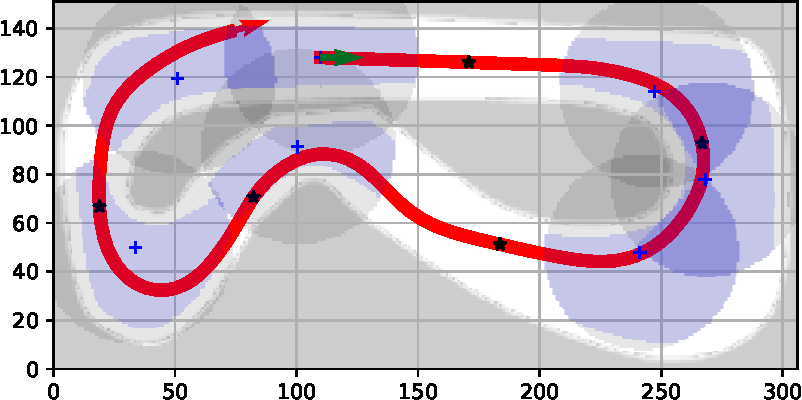
\includegraphics[width=\textwidth]{../img/experiments/porto-hybrid_astar-trajectory}
		\end{subfigure}
		\hfill
		\begin{subfigure}[c]{0.4\textwidth}
			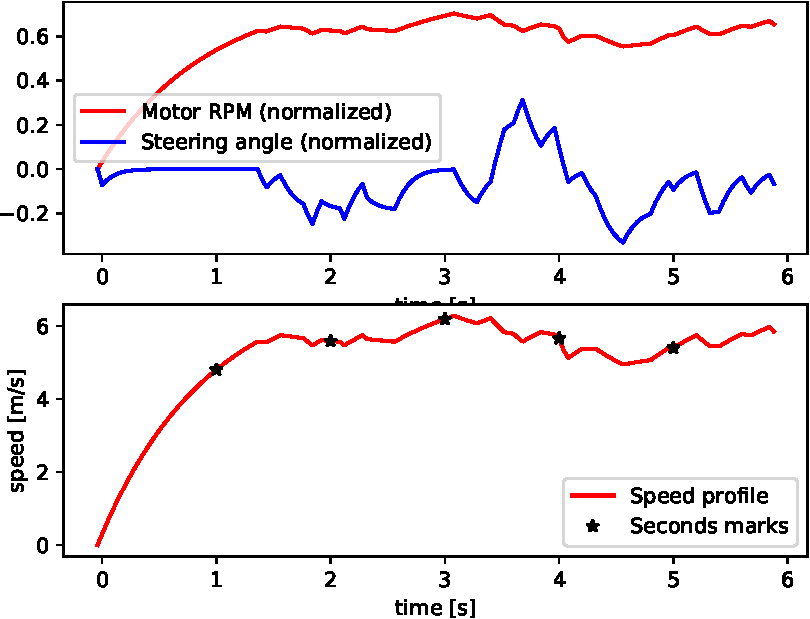
\includegraphics[width=\textwidth]{../img/experiments/porto-hybrid_astar-actuators}
		\end{subfigure}
		\caption{Solution found by Hybrid A*}
		\label{fig:solution_porto-hybrid_astar}	
	\end{subfigure}
	
	\vspace{0.75cm}
	
	\begin{subfigure}[t]{\textwidth}
		\begin{subfigure}[c]{0.59\textwidth}
			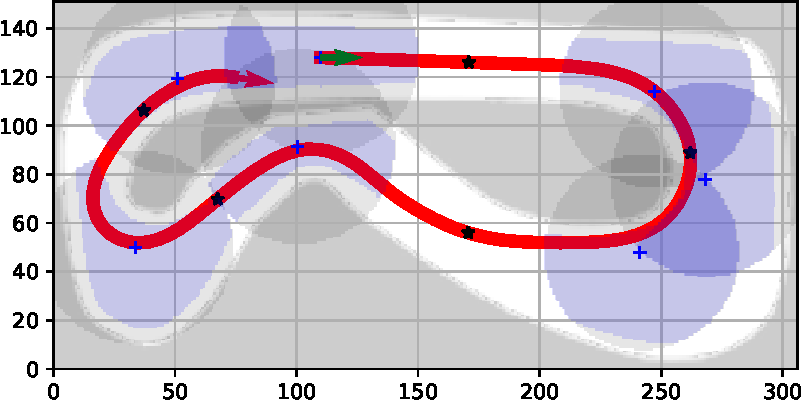
\includegraphics[width=\textwidth]{../img/experiments/porto-sehs-trajectory}
		\end{subfigure}
		\hfill
		\begin{subfigure}[c]{0.4\textwidth}
			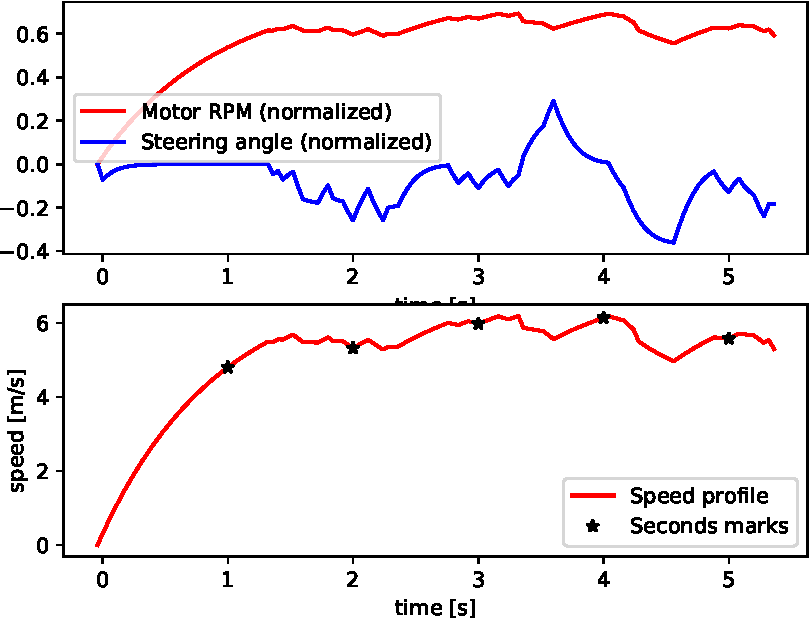
\includegraphics[width=\textwidth]{../img/experiments/porto-sehs-actuators}
		\end{subfigure}
		\caption{Solution found by SEHS}
		\label{fig:solution_porto-sehs}
	\end{subfigure}

	\vspace{0.75cm}
	
	\begin{subfigure}[t]{\textwidth}
		\centering
		\begin{tabular}{l r r r r r}%
			\toprule
			Algorithm & Opened & Expanded & Search time & Length & Lap time \\
			\midrule
			Hybrid A* & \num{504107} & \num{10324} & \SI{793.2}{\milli\second} & \SI{38.1}{\meter} & \bftab \SI{6.96}{\second} \\
			SEHS & \bftab \num{291687} & \bftab \num{5960} & \bftab \SI{563.0}{\milli\second} & \SI{40.1}{\meter} & \SI{7.08}{\second} \\
			\bottomrule
		\end{tabular}
		\caption{Comparison of the solutions and computation requirements.}
		\label{table:porto}
	\end{subfigure}

	\vspace{0.5cm}
	
	\caption{Track ``Porto''}
	\label{fig:porto}
\end{figure}


\begin{figure}[!tbp]%
	\centering
	
	\begin{subfigure}[t]{\textwidth}
		\begin{subfigure}[c]{0.54\textwidth}
			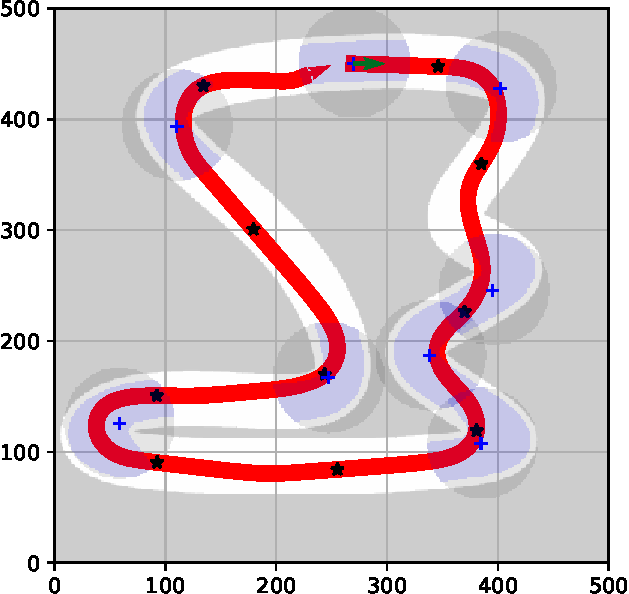
\includegraphics[width=\textwidth]{../img/experiments/tornado-hybrid_astar-trajectory}
		\end{subfigure}
		\hfill
		\begin{subfigure}[c]{0.45\textwidth}
			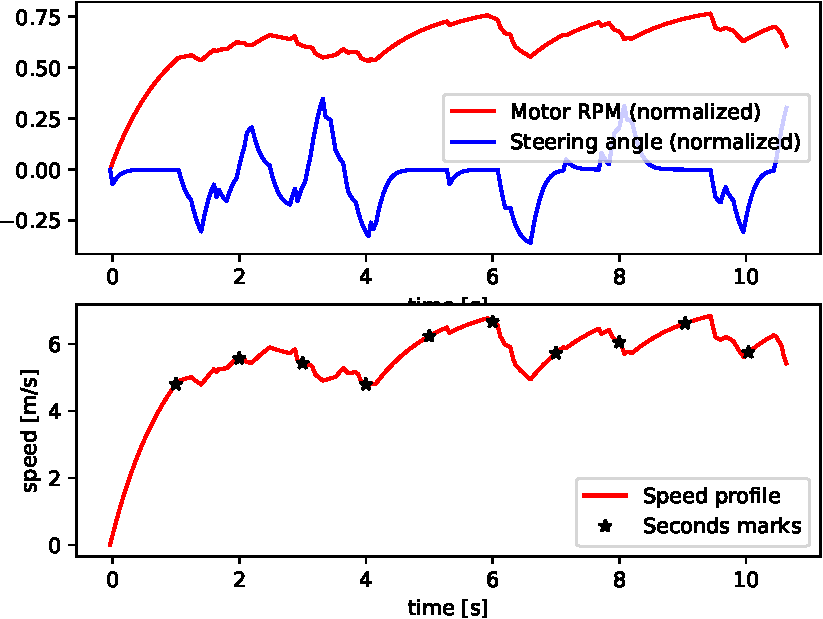
\includegraphics[width=\textwidth]{../img/experiments/tornado-hybrid_astar-actuators}
		\end{subfigure}
		\caption{Solution found by Hybrid A*}
		\label{fig:solution_tornado-hybrid_astar}	
	\end{subfigure}
	
	\vspace{0.75cm}
	
	\begin{subfigure}[t]{\textwidth}
		\begin{subfigure}[c]{0.54\textwidth}
			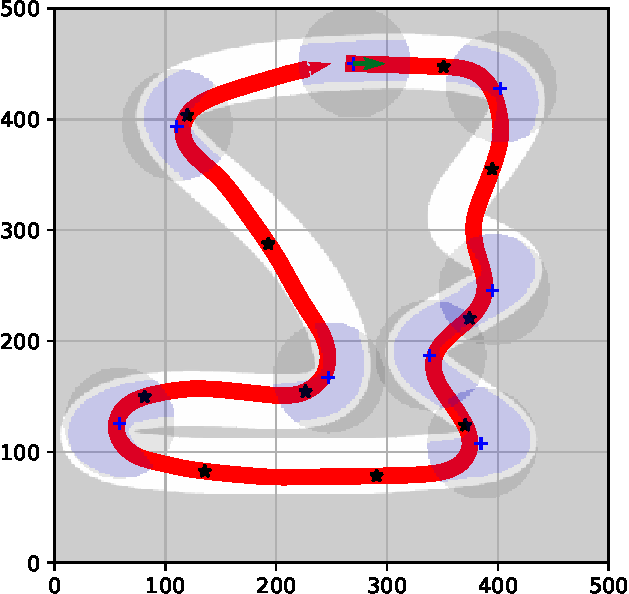
\includegraphics[width=\textwidth]{../img/experiments/tornado-sehs-trajectory}
		\end{subfigure}
		\hfill
		\begin{subfigure}[c]{0.45\textwidth}
			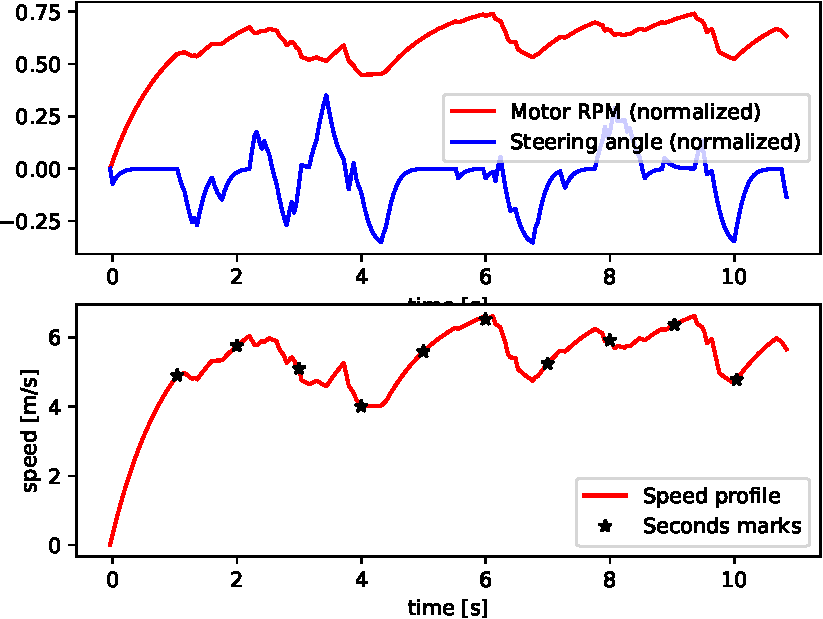
\includegraphics[width=\textwidth]{../img/experiments/tornado-sehs-actuators}
		\end{subfigure}
		\caption{Solution found by SEHS}
		\label{fig:solution_tornado-sehs}
	\end{subfigure}
	
	\vspace{0.75cm}
	
	\begin{subfigure}[t]{\textwidth}
		\centering
		\begin{tabular}{l r r r r r}%
			\toprule
			Algorithm & Opened & Expanded & Search time & Length & Lap time \\
			\midrule
			Hybrid A* & \num{4799135} & \num{108212} & \SI{12463.5}{\milli\second} & \SI{85.3}{\meter} & \SI{15.08}{\second} \\
			SEHS & \bftab \num{1147666} & \bftab \num{24285} & \bftab \SI{3153.5}{\milli\second} & \SI{83.2}{\meter} & \bftab \SI{14.28}{\second} \\
			\bottomrule
		\end{tabular}
		\caption{Comparison of the solutions and computation requirements.}
		\label{table:tornado}
	\end{subfigure}
	
	\vspace{0.75cm}
	
	\caption{Track ``Tornado''}
	\label{fig:tornado}
\end{figure}

\begin{figure}[!tbp]%
	\centering

	\begin{subfigure}[t]{\textwidth}
		\begin{subfigure}[c]{0.54\textwidth}
			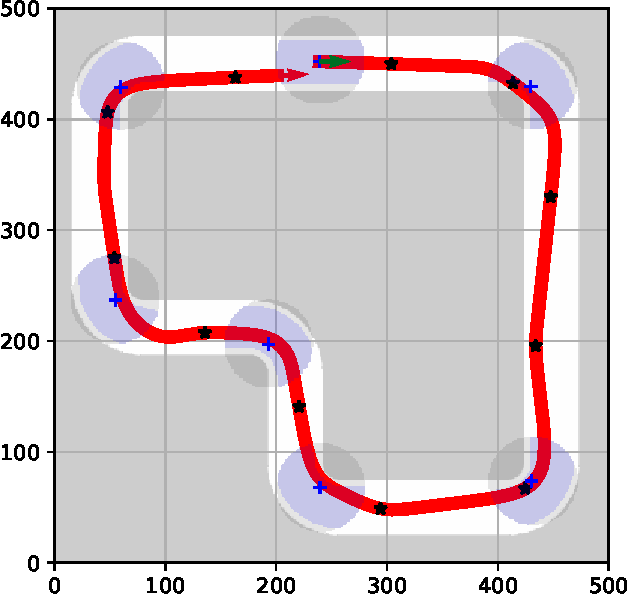
\includegraphics[width=\textwidth]{../img/experiments/simple-hybrid_astar-trajectory}
		\end{subfigure}
		\hfill
		\begin{subfigure}[c]{0.45\textwidth}
			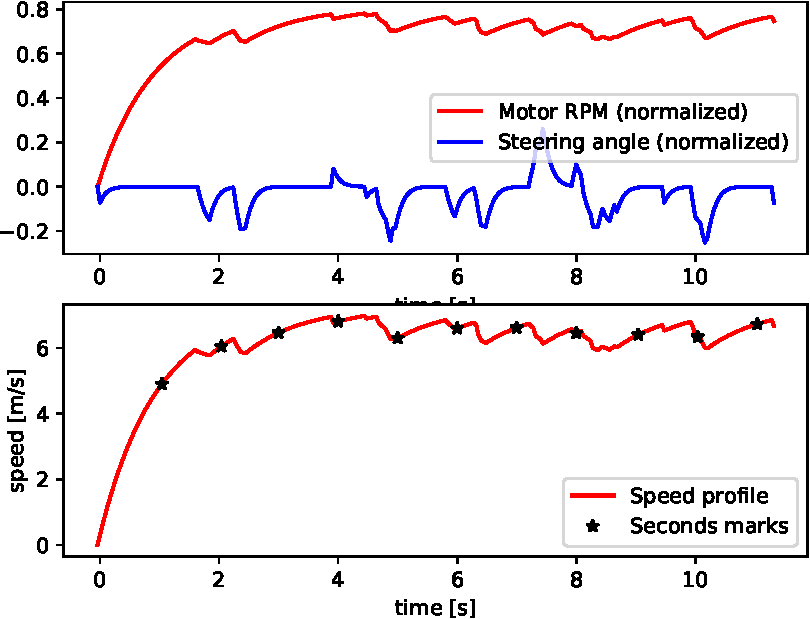
\includegraphics[width=\textwidth]{../img/experiments/simple-hybrid_astar-actuators}
		\end{subfigure}
		\caption{Solution found by Hybrid A*}
		\label{fig:simple-hybrid_astar}
	\end{subfigure}

	\vspace{0.75cm}
	
	\begin{subfigure}[t]{\textwidth}
		\begin{subfigure}[c]{0.54\textwidth}
			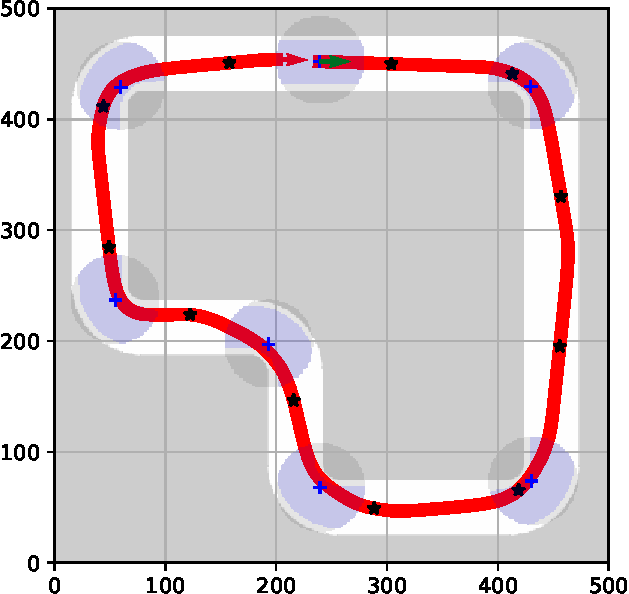
\includegraphics[width=\textwidth]{../img/experiments/simple-sehs-trajectory}
		\end{subfigure}
		\hfill
		\begin{subfigure}[c]{0.45\textwidth}
			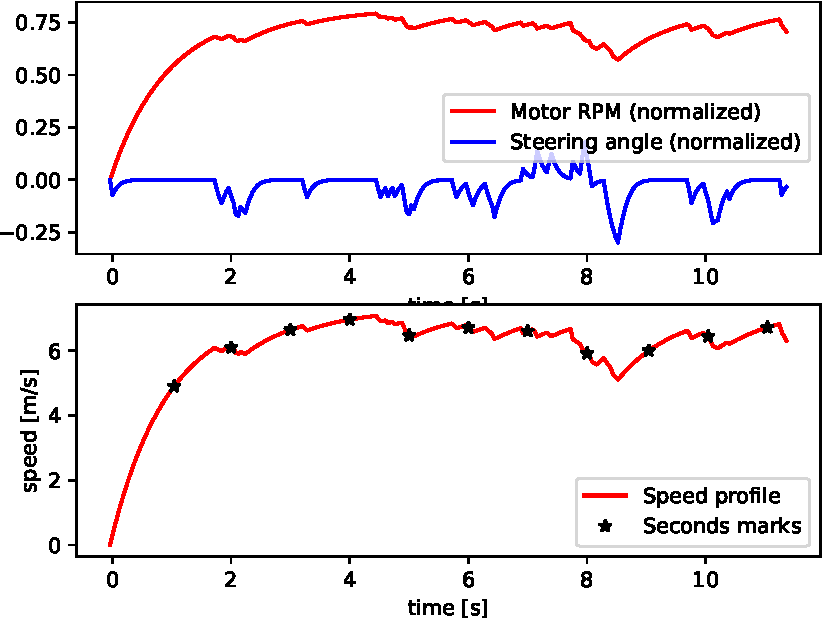
\includegraphics[width=\textwidth]{../img/experiments/simple-sehs-actuators}
		\end{subfigure}
		\caption{Solution found by SEHS}
		\label{fig:simple-sehs}
	\end{subfigure}

	\vspace{0.75cm}

	\begin{subfigure}[t]{\textwidth}
		\centering
		\begin{tabular}{l r r r r r}%
			\toprule
			Algorithm & Opened & Expanded & Search time & Length & Lap time \\
			\midrule
			Hybrid A* & \num{588820} & \num{13700} & \SI{1193.2}{\milli\second} & \SI{68.7}{\meter} & \bftab \SI{11.44}{\second} \\
			SEHS & \bftab \num{404326} & \bftab \num{8737} & \bftab \SI{956.4}{\milli\second} &  \SI{68.5}{\meter} & \bftab \SI{11.52}{\second} \\
			\bottomrule
		\end{tabular}
		\caption{Comparison of the solutions and computation requirements.}
		\label{table:simple}
	\end{subfigure}
	
	\vspace{0.75cm}

	\caption{Track ``Simple''}
	\label{fig:simple}
\end{figure}

\begin{figure}[!tbp]%
	\centering

	\begin{subfigure}[t]{\textwidth}
		\begin{subfigure}[c]{0.54\textwidth}
			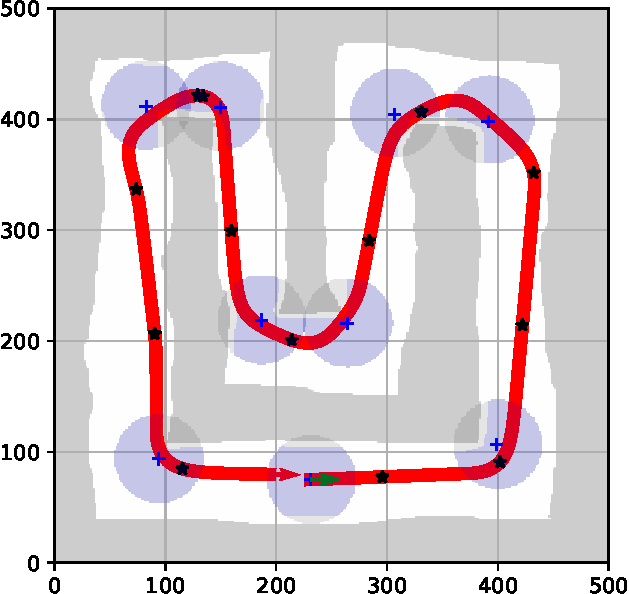
\includegraphics[width=\textwidth]{../img/experiments/u-hybrid_astar-trajectory}
		\end{subfigure}
		\hfill
		\begin{subfigure}[c]{0.45\textwidth}
			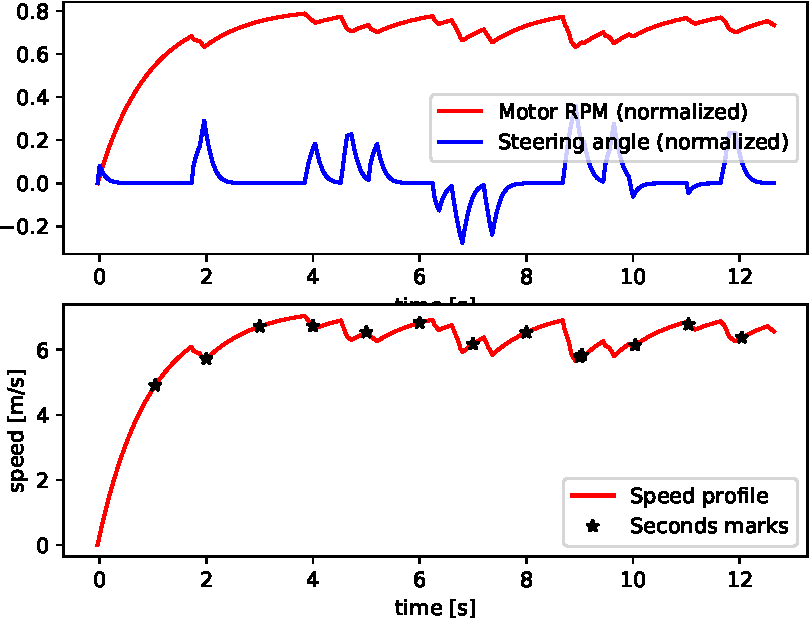
\includegraphics[width=\textwidth]{../img/experiments/u-hybrid_astar-actuators}
		\end{subfigure}	
		\caption{Solution found by Hybrid A*}
		\label{fig:u-hybrid_astar}
	\end{subfigure}

	\vspace{0.75cm}

	\begin{subfigure}[t]{\textwidth}
		\begin{subfigure}[c]{0.54\textwidth}
			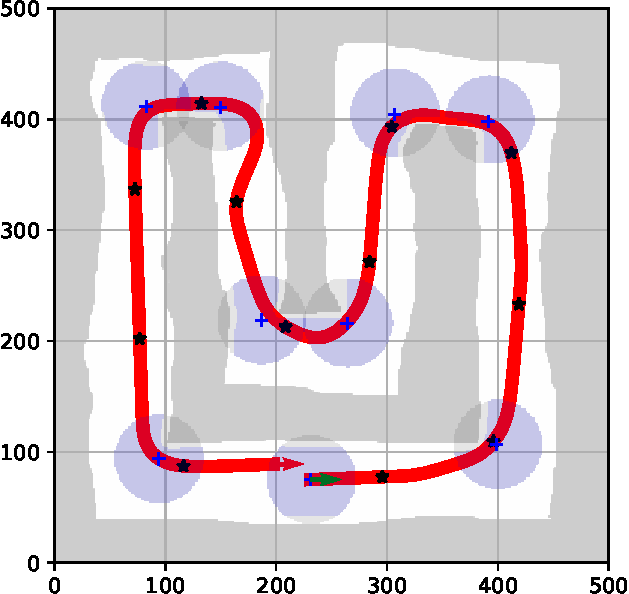
\includegraphics[width=\textwidth]{../img/experiments/u-sehs-trajectory}
		\end{subfigure}
		\hfill
		\begin{subfigure}[c]{0.45\textwidth}
			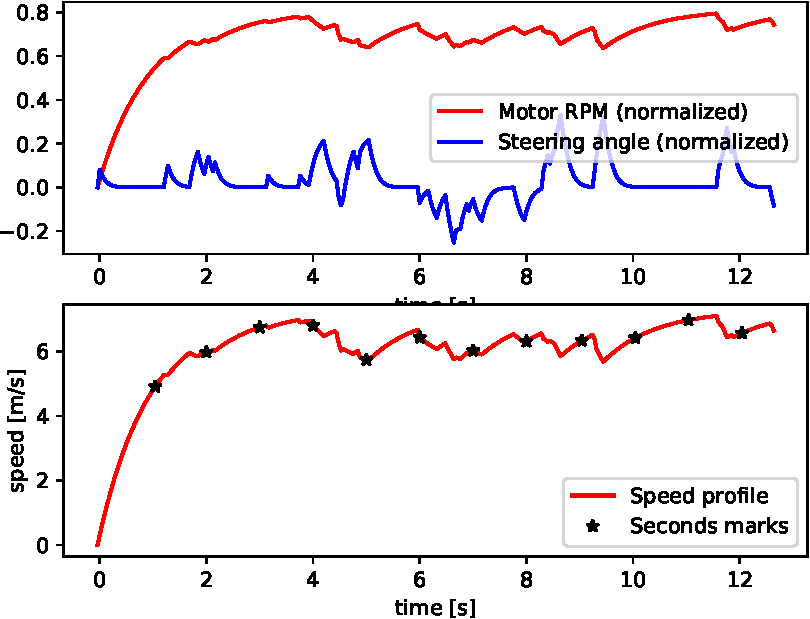
\includegraphics[width=\textwidth]{../img/experiments/u-sehs-actuators}
		\end{subfigure}
		\caption{Solution found by SEHS}
		\label{fig:u-sehs}
	\end{subfigure}
	
	\vspace{0.75cm}
	
	\begin{subfigure}[t]{\textwidth}
		\centering
		\begin{tabular}{l r r r r r}%
		\toprule
		Algorithm & Opened & Expanded & Search time & Length & Lap time \\
		\midrule
		Hybrid A* & \num{2728137} & \num{58495} & \SI{6441.4}{\milli\second} & \SI{73.1}{\meter} & \bftab \SI{12.52}{\second} \\
		SEHS & \bftab \num{1201905} & \bftab \num{25363} & \bftab \SI{3381.7}{\milli\second} & \SI{72.6}{\meter} & \SI{12.64}{\second} \\
		\bottomrule
	\end{tabular}
	\caption{Comparison of the solutions and computation requirements.}
	\label{table:u}
	\end{subfigure}
	
	\vspace{0.75cm}
	
	\caption{Track ``U''}
	\label{fig:u}
\end{figure}

\begin{figure}[!tbp]%
	\centering
		
	\begin{subfigure}[t]{\textwidth}
		\begin{subfigure}[c]{0.54\textwidth}
			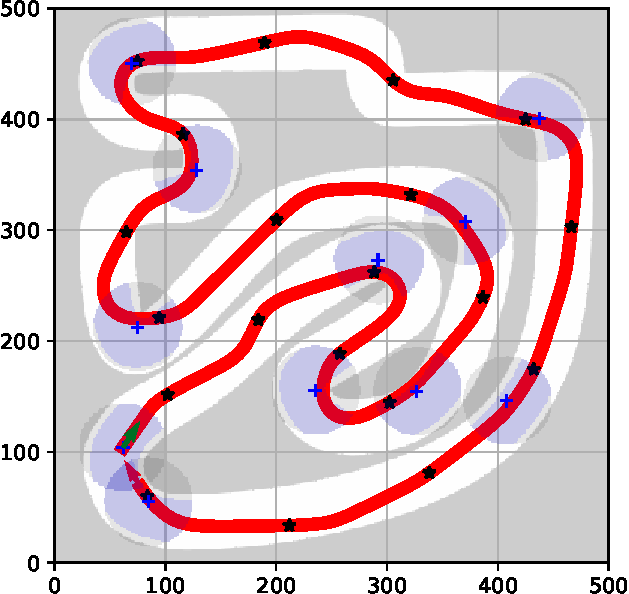
\includegraphics[width=\textwidth]{../img/experiments/zurich-hybrid_astar-trajectory}
		\end{subfigure}
		\hfill
		\begin{subfigure}[c]{0.45\textwidth}
			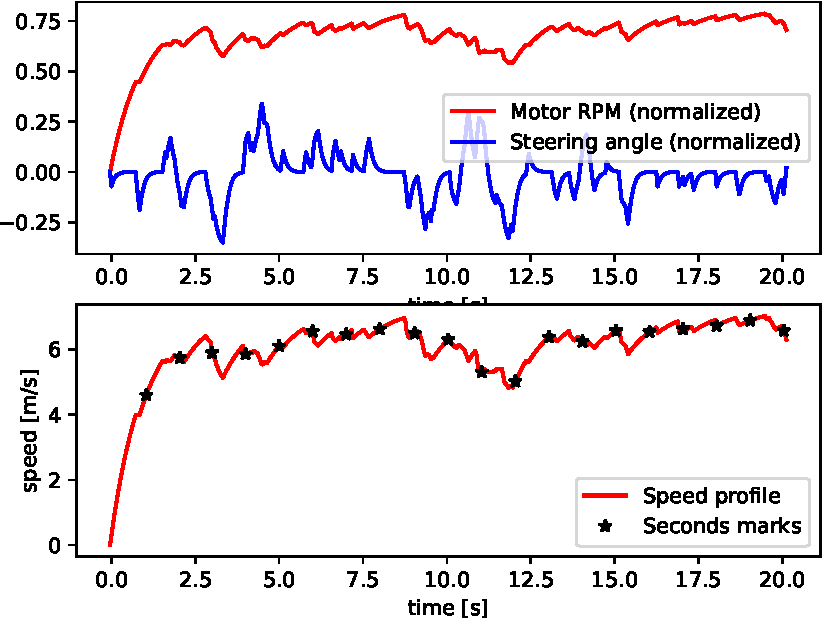
\includegraphics[width=\textwidth]{../img/experiments/zurich-hybrid_astar-actuators}
		\end{subfigure}
		\caption{Solution found by Hybrid A*}
		\label{fig:zurich-hybrid_astar}
	\end{subfigure}

	\vspace{0.75cm}
	
	\begin{subfigure}[t]{\textwidth}	
		\begin{subfigure}[c]{0.54\textwidth}
			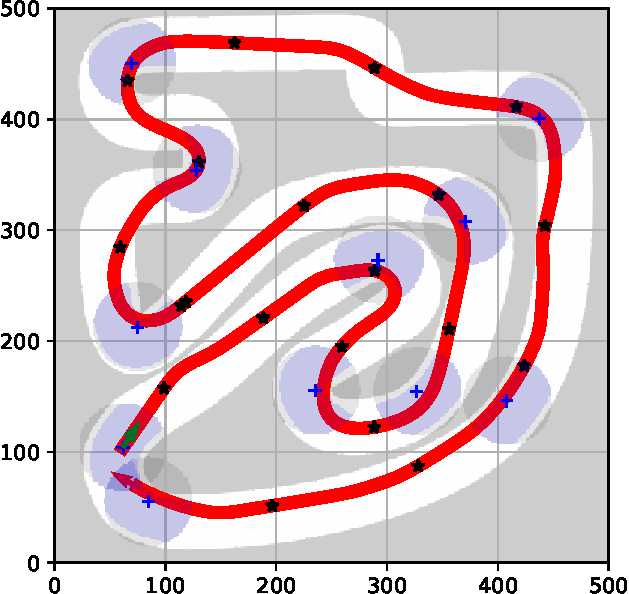
\includegraphics[width=\textwidth]{../img/experiments/zurich-sehs-trajectory}
		\end{subfigure}
		\hfill
		\begin{subfigure}[c]{0.45\textwidth}
			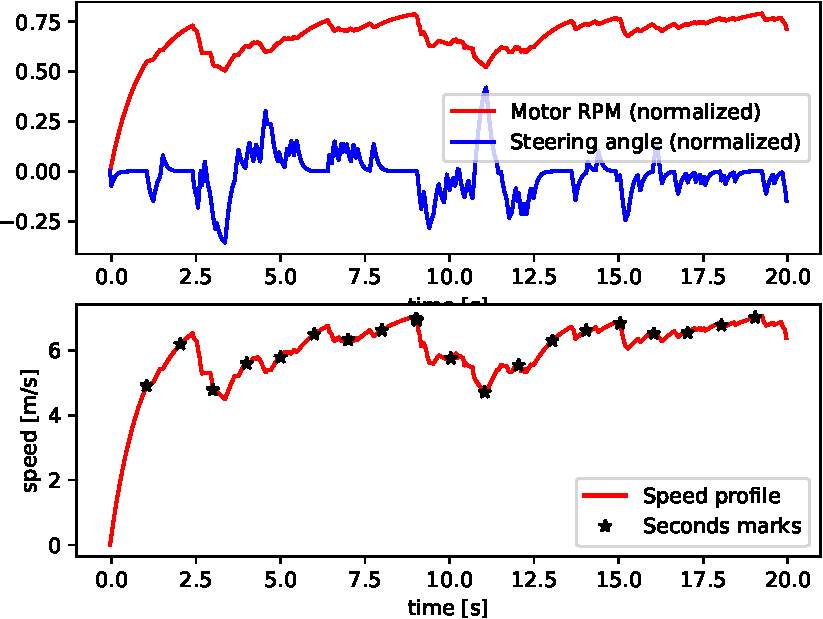
\includegraphics[width=\textwidth]{../img/experiments/zurich-sehs-actuators}
		\end{subfigure}
		\caption{Solution found by SEHS}
		\label{fig:zurich-sehs}
	\end{subfigure}

	\vspace{0.75cm}
	
	\begin{subfigure}[t]{\textwidth}
		\centering
		\begin{tabular}{l r r r r r}%
			\toprule
			Algorithm & Opened & Expanded & Search time & Length & Lap time \\
			\midrule
			Hybrid A* & \num{3877615} & \num{90808} & \SI{9778.2}{\milli\second} & \SI{117.8}{\meter} & \SI{20.0}{\second} \\
			\gls*{SEHS} & \bftab \num{1602588} & \bftab \num{37000} & \bftab \SI{5483.6}{\milli\second} & \SI{116.5}{\meter} & \SI{20.0}{\second} \\
			\bottomrule
		\end{tabular}
		\caption{Comparison of the solutions and computation requirements.}
		\label{table:zurich}
	\end{subfigure}
	
	\vspace{0.75cm}

	\caption{Track ``Zurich''}
	\label{fig:zurich}
\end{figure}

\begin{figure}[!tbp]%
	\centering
	
	\begin{subfigure}[t]{\textwidth}
		\begin{subfigure}[c]{0.54\textwidth}
			\includegraphics[width=\textwidth]{../img/experiments/race_track-hybrid_astar-trajectory}
		\end{subfigure}
		\hfill
		\begin{subfigure}[c]{0.45\textwidth}
			\includegraphics[width=\textwidth]{../img/experiments/race_track-hybrid_astar-actuators}
		\end{subfigure}
		\caption{Solution found by Hybrid A*}
		\label{fig:race_track-hybrid_astar}
	\end{subfigure}
	
	\vspace{0.75cm}
	
	\begin{subfigure}[t]{\textwidth}	
		\begin{subfigure}[c]{0.54\textwidth}
			\includegraphics[width=\textwidth]{../img/experiments/race_track-sehs-trajectory}
		\end{subfigure}
		\hfill
		\begin{subfigure}[c]{0.45\textwidth}
			\includegraphics[width=\textwidth]{../img/experiments/race_track-sehs-actuators}
		\end{subfigure}
		\caption{Solution found by SEHS}
		\label{fig:race_track-sehs}
	\end{subfigure}
	
	\vspace{0.75cm}
	
	\begin{subfigure}[t]{\textwidth}
		\centering
		\begin{tabular}{l r r r r r}%
			\toprule
			Algorithm & Opened & Expanded & Search time & Length & Lap time \\
			\midrule
			Hybrid A* & \num{2389238} & \num{54269} & \bftab \SI{5718.0}{\milli\second} & \SI{80.3}{\meter} & \bftab \SI{13.8}{\second} \\
			\gls*{SEHS} & \bftab \num{2098623} & \bftab \num{44951} & \SI{6391.0}{\milli\second} & \SI{81.7}{\meter} & \SI{14.4}{\second} \\
			\bottomrule
		\end{tabular}
		\caption{Comparison of the solutions and computation requirements.}
		\label{table:race_track}
	\end{subfigure}
	
	\vspace{0.75cm}
	
	\caption{Track ``Race Track''}
	\label{fig:race_track}
\end{figure}

\section{Autonomous Race}

To further test the algorithms, we implemented the complete Artificial Racing Agent on top of the \gls{ROS} and we built a custom hardware inspired by the F1/10 platform. The details of the implementation are described in the appendixes Experimental Vehicle (Appendix~\ref{chapter:hardware}) and Technical Documentation (Appendix~\ref{chapter:technical_documentation}).

In the following experiments, we tried to test the racing capabilities of the vehicle. The vehicle was given a complete map of the circuit at the beginning of the race. The goal was to go around the circuit repeatedly without colliding with walls and obstacles and reaching the best lap times as possible.

The agent repeatedly triggers the \gls{SEHS} based trajectory planning algorithm from the latest known state of the vehicle with the latest known state of the map with the obstacles marked in it through the current list of waypoints. At the same time, the vehicle is already driving and following the last published trajectory. Once the planning algorithm comes up with a new plan, it replaces the old plan and it can start planning again with the latest known state.

\subsection{Testing Criteria}
For the planning algorithm to be viable, it must calculate the trajectory in a short period of time before the vehicle physically moves to the end of the previous trajectory. We were also interested in the safety of the planned trajectory and the distance the vehicle keeps from the obstacles while following the trajectory. Finally, our goal is to achieve fast lap times and we are interested in the maximum speed our vehicle can achieve while driving safely.

\subsection{Real World Testing}

\begin{figure}
	\label{fig:real-world-testing-still}
	\centering
	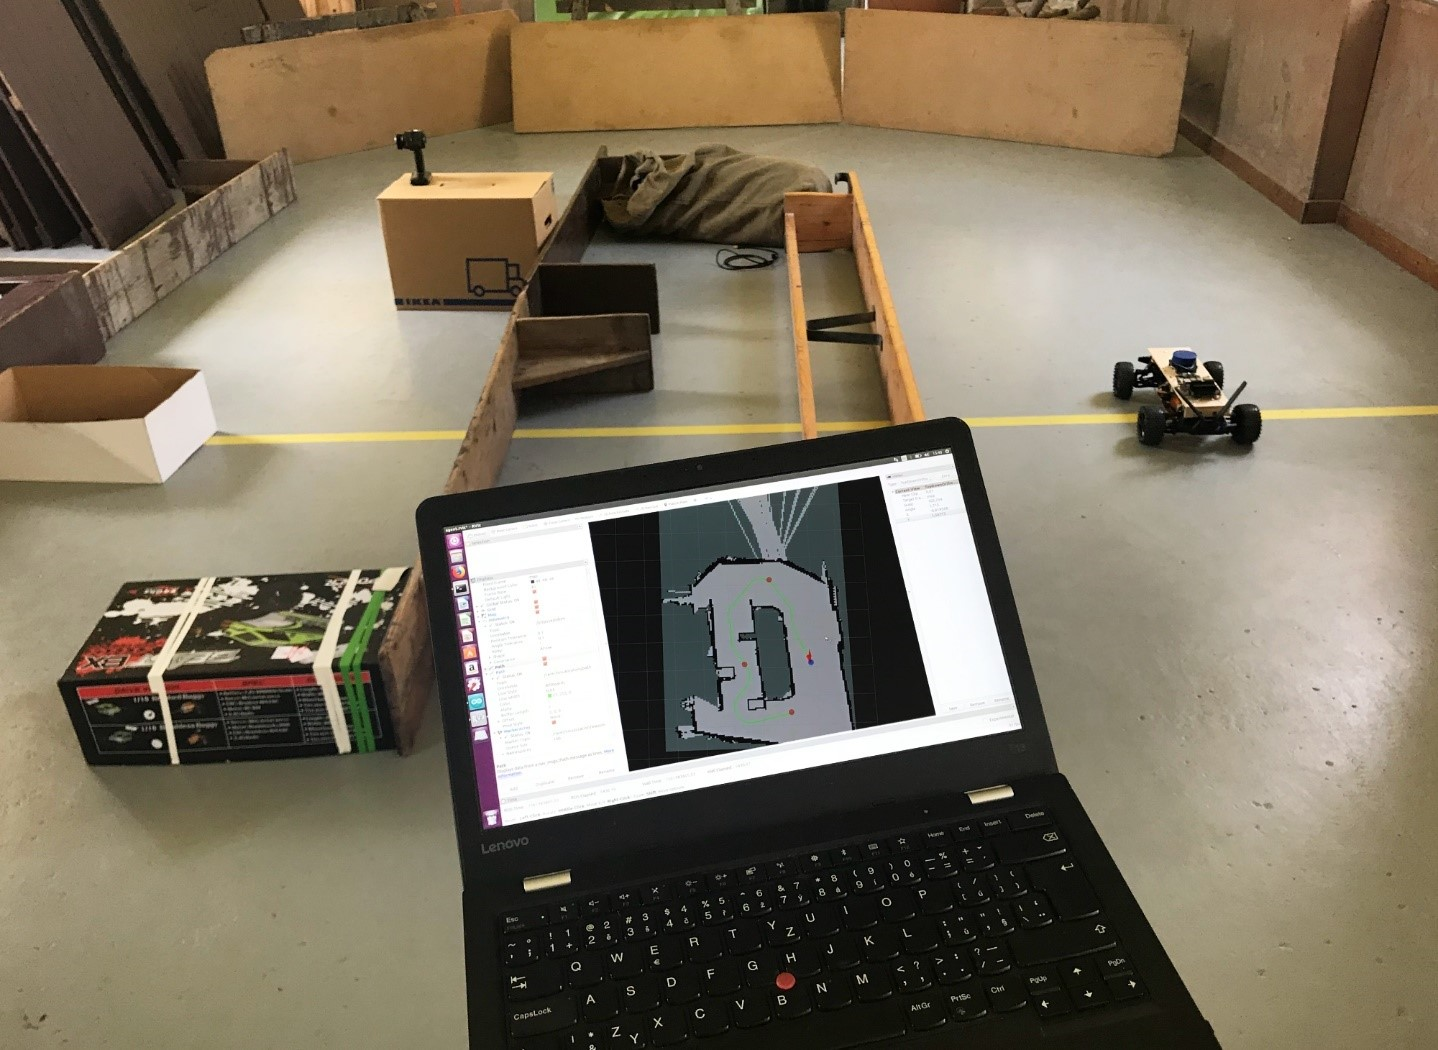
\includegraphics[width=\textwidth]{../img/experiments/real-world-still.jpg}
	\caption{The planning algorithm finds a trajectory from the last known state of the vehicle through the waypoints ahead of it while avoiding the obstacles marked in the map.}
\end{figure}


Initially, we wanted to perform tests outdoors on an asphalt plane, but it proved problematic because of surface curvature and unstable weather conditions. Another unexpected problem we had to solve was a problem with the \gls*{LIDAR} unit. It performed very unreliably in direct sunlight. In the end, we tested our vehicle indoors in a rectangular gym \SI{10}{\meter} long and \SI{6}{\meter} wide with concrete surface which was available to us for several days. We built several versions of an obstacle course using gym equipment and from cardboard boxes. One such circuit is shown in Figure~\ref{fig:real-world-testing-still}.

The experiment consisted of two phases. First, we built a 2D map from the data coming from the \gls*{LIDAR} as the vehicle drove around the track using a remote controller. Using this map, we assembled a configuration file describing the racing circuit. Next, we started all the \gls{ROS} nodes for vehicle state monitoring, circuit progress monitoring, trajectory planning, and trajectory following. Once the planning algorithm produces the first trajectory, the vehicle would start following it. We were closely monitoring the movement of the vehicle visually and using telemetry data on a laptop through the \texttt{Rviz} program\footnote{\url{http://wiki.ros.org/rviz}}. We were always ready to take control of the vehicle using the remote control to prevent damage to the vehicle and to its surroundings. Any input from the controller would cancel the autonomous mode and switch the vehicle into a remote-control mode. The vehicle then stayed in this mode until a button on the vehicle was physically pressed.

We struggled with unreliable odometry for several days. We tested several different localization libraries, adjusted data collected from the sensors, and tweaked the parameters of the libraries until we were able to get usable odometry data at least at low speeds. At higher speeds, the vehicle would quickly lose track of its actual position and orientation on the map and it would collide with a wall or with an obstacle.

By the end of the testing, the vehicle was able to reliably circle around the track without hitting obstacles and without the odometry significantly diverging from the actual state of the vehicle. The car repeatedly completed a circuit which was approximately 20 meters long in 15 seconds at a steady speed of \SI{1.3}{\meter\per\second}~(\SI{4.68}{\kilo\meter\per\hour}) which corresponds to a speed of \SI{46.8}{\kilo\meter\per\hour} of a full-size vehicle. At this speed, the limitations of the kinematic model do not manifest, and the vehicle had no issues undershooting or overshooting turns. A photo from this test is shown in Figure~\ref{fig:real-world-testing-driving} and a video recording of this experiment is available in the attachment of this thesis \todo{Add the path to the file in a footnote}.

\begin{figure}
	\label{fig:real-world-testing-driving}
	\centering
	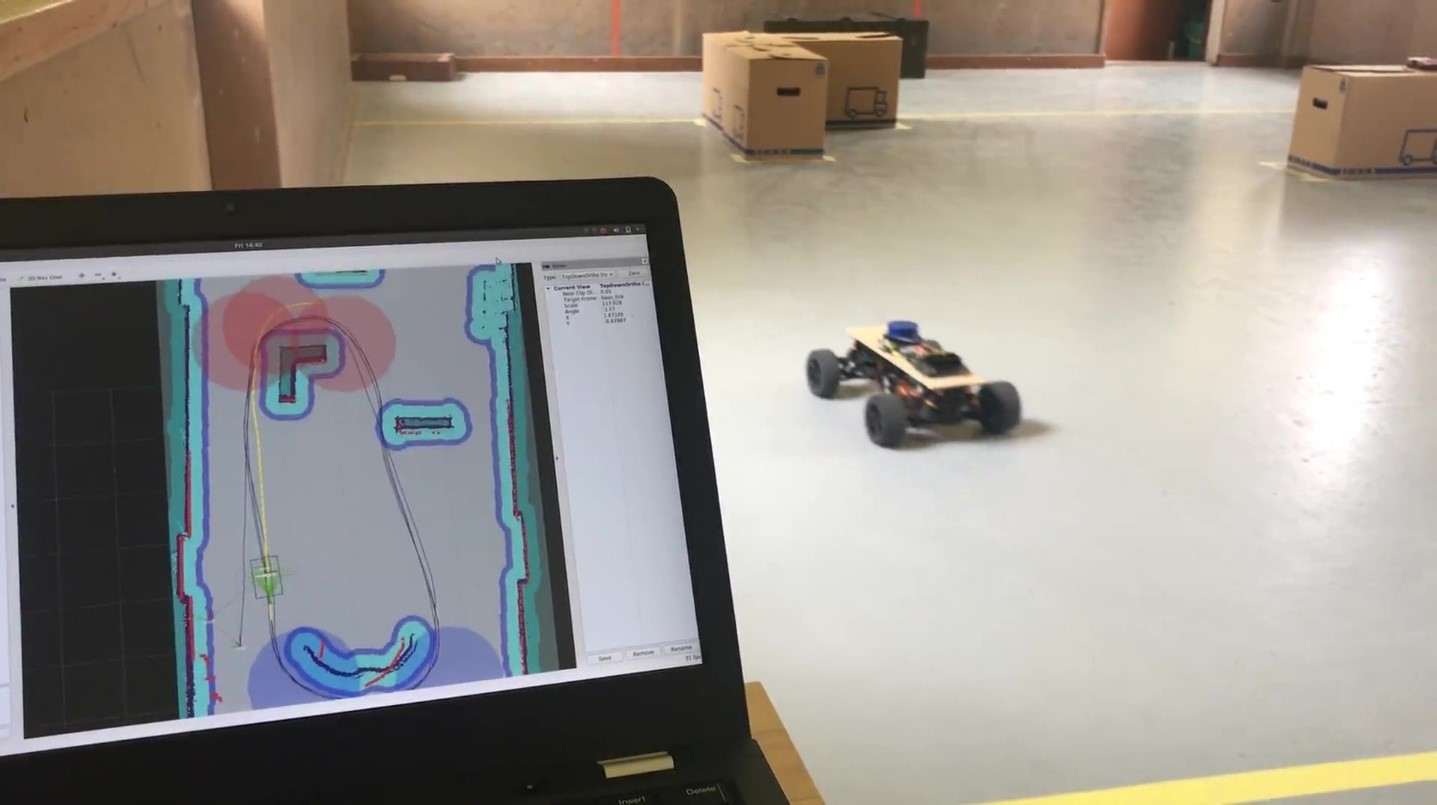
\includegraphics[width=\textwidth]{../img/experiments/real-world-driving.jpg}
	\caption{The vehicle is slowly driving along a circuit in a gym. The telemetry from the vehicle is monitored on a notebook connected to the vehicle over Wi-Fi.}
\end{figure}

The trajectory planning algorithm performed well even with just the low-powered ARM processor and the vehicle had never reached the end of the planned trajectory before a new extended trajectory was published. The \gls{DWA} algorithm kept the vehicle on the track and avoided all crates along the circuit.

Although the robot was able to navigate autonomously without collisions, the speeds we were able to reach were too low and did not reach a speed at which we would start seeing any effects of high speed maneuvers, such as wheel slipping and skidding and overshooting corners. We were also unable to test evasion of dynamic obstacles because the obstacle detection library produced too many ghost obstacles from our noisy and low-frequency \gls*{LIDAR} scans.

\subsection{Simulator}
Due to the hardware issues we ran into and due to other factors, which did not allow further improvements and testing of the vehicle during the spring of 2020, we conducted further experiments only with the Gazebo simulator \cite{gazebo} configured for the F1/10 platform \cite{varundev_ros_19}. This change gave us the opportunity to test the algorithm with perfect odometry, but with the same interface between the algorithm and the simulated actuators of the virtual vehicle. To adapt the algorithm for the simulator, we had to modify our steering servo and motor models. We tweaked the parameters of our models to predict the behavior of the simulated vehicle as closely as possible.

The F1/10 simulator repository\footnote{\url{https://github.com/f1tenth-dev/simulator}} contains a 3D map with several different types of corners and it is shown in Figure~\ref{fig:gazebo-track}. Especially the middle part which consists of a series of left-hand turn followed by a right-hand hairpin turn presents a challenge where the car must slow down to avoid collision while keeping as much speed as possible to still reach a good lap time. We ran the full-circuit planning for the modified vehicle model and for this track. The planned trajectories are shown in Figure~\ref{fig:sim-race_track}.


\begin{figure}[!tbp]%
	\centering
	
	\begin{subfigure}[t]{\textwidth}
		\begin{subfigure}[c]{0.54\textwidth}
			\includegraphics[width=\textwidth]{../img/experiments/sim-race_track-hybrid_astar-trajectory}
		\end{subfigure}
		\hfill
		\begin{subfigure}[c]{0.45\textwidth}
			\includegraphics[width=\textwidth]{../img/experiments/sim-race_track-hybrid_astar-actuators}
		\end{subfigure}
		\caption{Solution found by Hybrid A*}
		\label{fig:sim-race_track-hybrid_astar}
	\end{subfigure}
	
	\vspace{0.75cm}
	
	\begin{subfigure}[t]{\textwidth}	
		\begin{subfigure}[c]{0.54\textwidth}
			\includegraphics[width=\textwidth]{../img/experiments/sim-race_track-sehs-trajectory}
		\end{subfigure}
		\hfill
		\begin{subfigure}[c]{0.45\textwidth}
			\includegraphics[width=\textwidth]{../img/experiments/sim-race_track-sehs-actuators}
		\end{subfigure}
		\caption{Solution found by SEHS}
		\label{fig:sim-race_track-sehs}
	\end{subfigure}
	
	\vspace{0.75cm}
	
	\begin{subfigure}[t]{\textwidth}
		\centering
		\begin{tabular}{l r r r r r}%
			\toprule
			Algorithm & Opened & Expanded & Search time & Length & Lap time \\
			\midrule
			Hybrid A* & \num{414589} & \num{10772} & \bftab \SI{1013.4}{\milli\second} & \SI{83.9}{\meter} & \SI{14.16}{\second} \\
			\gls*{SEHS} & \bftab \num{356968} & \bftab \num{8524} & \SI{1111.6}{\milli\second} & \SI{85.5}{\meter} & \bftab \SI{13.24}{\second} \\
			\bottomrule
		\end{tabular}
		\caption{}
		\label{table:sim-race_track}
	\end{subfigure}
	
	\vspace{0.75cm}
	
	\caption{The planning algorithms executed with the modified model of the simulated vehicle on the ``Race Track``. When compared to Figure~\ref{fig:race_track}, there is an apparent difference in braking around the hairpin turn in the middle section of the track.}
	\label{fig:sim-race_track}
\end{figure}

For this experiment, we turned off obstacle detection and we focused only on the lap times in a track without any obstacles. We tried three different algorithms and for each of them, we let it run for up to 10 consecutive laps. We ran each algorithm three times and we used the run in which it was able to complete all of the 10 laps and in which it reached the best average lap time.

\begin{figure}
	\label{fig:gazebo-track}
	\centering
	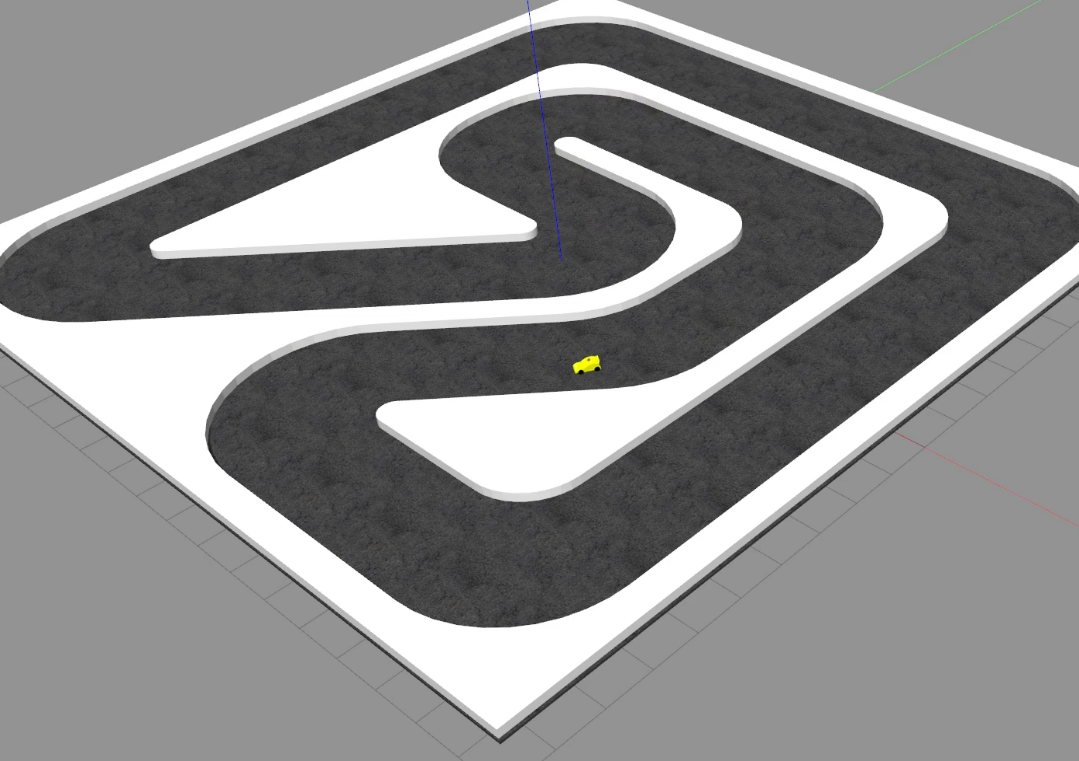
\includegraphics[width=\textwidth]{../img/experiments/gazebo-track.png}
	\caption{The testing track contains several long straights and several challenging turns. The Gazebo simulator allows us to monitor and modify the 3D scene.}
\end{figure}

\begin{figure}
	\label{fig:rviz-planned-track}
	\centering
	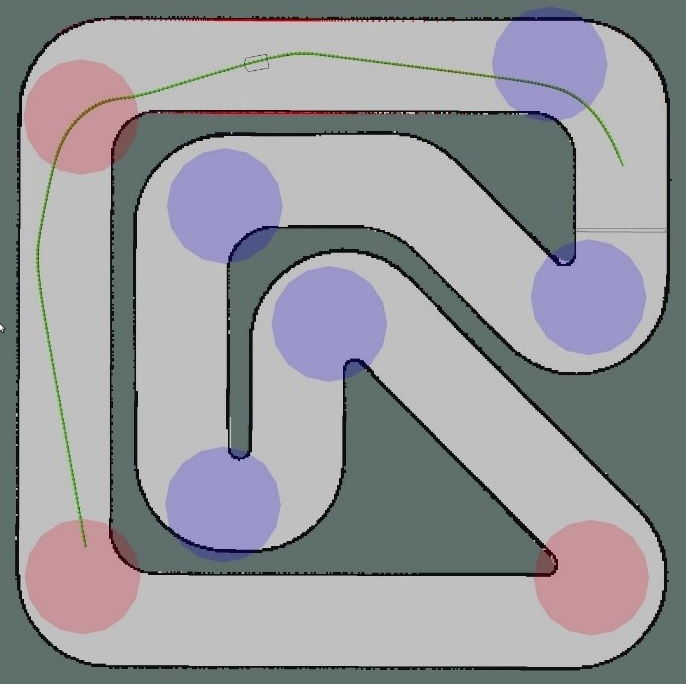
\includegraphics[width=\textwidth]{../img/experiments/rviz-planned-track.jpg}
	\caption{This figure captures a planned trajectory and a vehicle on the testing track as it is shown in Rviz. The circles represent the positions of the corners detected by the track analysis algorithm. The circles marked in red are the next three corners ahead of the vehicle. The mostly green line represents the last planned trajectory. Green parts of the trajectory show where the vehicle is expected to drive fast and red parts would show where the vehicle should slow down.}
\end{figure}

\paragraph{Reference Implementation}
The F1/10 Simulator repository contains a reference implementation of the Pure Pursuit algorithm which follows a fixed spline path divided sectors marked as “unrestricted”, “caution”, and “brake”, which tell the vehicle how to adjust its speed. We used this implementation as a baseline and we will compare our results against this implementation. This algorithm cannot react to any unexpected obstacles.

\paragraph{\gls{SEHS} and Pure Pursuit}
The first trajectory following algorithm we tested was the combination of the \gls*{SEHS} planning algorithm and the Pure Pursuit controller. We tested different values of the lookahead distance, and we settled on an adaptive look ahead distance linearly proportional to the speed of the vehicle. The lookahead was set to \SI{0.5}{\meter} for a stopped vehicle and \SI{2.0}{\meter} for the theoretical top speed. This algorithm has no mechanism of avoiding unexpected obstacles which were not considered by the planning algorithm and pure pursuit would blindly hit an obstacle if the reference trajectory went through it.

\paragraph{\gls{SEHS} and \gls{DWA}}
The other controller we tested was the \gls{DWA} algorithm. This algorithm has several parameters which we tuned until we reached satisfying results. First parameter is the prediction horizon which determines for how long we predict the movement of the vehicle from the current measured state with a single examined action. Short prediction horizon does not give enough room to reveal differences between all the applicable actions and a long prediction horizon is unrealistic, because we change the action several times per second and it also eliminates many actions, because fixating one action for too long would likely lead to a collision. We achieved best results by setting the prediction horizon to \SI{0.3}{\second}.

The other parameters are the weights we assign to the error of the position of the vehicle, the error of its heading angle, the error of the speed of the vehicle, and the proximity to the obstacles ahead of the vehicle and nearby obstacles. In the end, the highest weight was assigned to the distance from obstacles and the second largest to the position error.

Thanks to the fact the obstacle proximity factor, which is considered by the \gls*{DWA} algorithm, it can steer the vehicle around obstacles which are detected using the \gls*{LIDAR} scans. We tested this by placing cubes and cylinders on the track in the Gazebo application. We tried placing the obstacles in several different ways. We tried blocking the apexes of a corner and forcing the vehicle to go along the outer wall. We also placed two boxes along each side of the track and forced the vehicle to go through a narrow gap in the middle. The third experiment with obstacles consisted of placing three boxes one after each other at sides of the track in an alternating pattern to block passage in a straight line. The success of avoidance was significantly impacted by the prediction horizon parameter. When this parameter was too short, the vehicle would notice the obstacle too late and it would not have enough room to avoid it and it would collide.

The planning algorithm could fail when the occasional misalignment of the \gls*{LIDAR} scans with the map caused ghost obstacles around the actual obstacles and around the walls being marked in the occupancy grid. Especially in the scenario with a narrow passage between two boxes, the track would seem completely blocked to the planning algorithm and it would not be able to produce a reference trajectory. We managed to reduce this effect by tuning the parameters of the obstacle detection library, but we were not able to eliminate this problem.

\paragraph{Results}

The simulated vehicle follows this trajectory almost flawlessly and during a test run of 10 consecutive laps it reached an average lap time of \SI{26.410}{\second} with top speed reaching \SI{4.08}{\meter\per\second} and the best lap time in this run was \SI{25.911}{\second}. For detailed statistics of lap times and speeds achieved by this algorithm, see Table~\ref{tbl:reference-impl}.

The trajectory analysis algorithm correctly detects eight corners of the circuit. We set the planning algorithm to plan for the next 3 corners ahead of it. The planning time on the desktop computer ranged between \SI{60}{\milli\second} and \SI{100}{\milli\second} depending on the initial state and on the length and complexity of the circuit segment ahead of the vehicle.

In our test, the \gls*{DWA} algorithm was achieve an average lap time of \SI{26.239}{\s} with the best lap time of \SI{23.855}{\s} and reaching a top speed of \SI{4.08}{\meter\per\second}. The Pure Pursuit algorithm achieved an average lap time of \SI{28.319}{\s} with the best lap time of \SI{26.908}{\s} and reaching a top speed of \SI{4.00}{\meter\per\second}. The detailed results of the experiment can be seen in Table~\ref{tbl:dwa} and Table~\ref{tbl:pure-pursuit}.

These times are still much slower than the planned lap times as shown in Table~\ref{table:sim-race_track}. The vehicle is clearly not able to reach the speeds predicted by the motor model. \todo[inline]{This is way off. I must really revisit this.}

\begin{table}
	\centering
	\label{tbl:reference-impl}
	\begin{tabular}{c c c c c}
		\toprule
		& Lap time       & Distance traveled  & Average speed             & Maximum speed             \\
		& [\si{\second}] & [\si{\meter}]      & [\si{\meter\per\second}]  & [\si{\meter\per\second}]  \\
		\midrule
		1. & 27.876 & 84.72 & 3.25 & 4.06 \\
		2. & 26.208 & 87.07 & 3.37 & 4.08 \\
		3. & 26.381 & 86.91 & 3.38 & 4.07 \\
		4. & 26.279 & 86.75 & 3.36 & 4.06 \\
		5. & 26.484 & 87.00 & 3.35 & 4.05 \\
		6. & 26.172 & 86.96 & 3.37 & 4.07 \\
		7. & 26.366 & 87.03 & 3.37 & 4.07 \\
		8. & 26.227 & 86.54 & 3.37 & 4.08 \\
		9. & \textbf{25.911} & \textbf{85.83} & \textbf{3.37} & \textbf{4.05} \\
		10. & 26.199 & 86.39 & 3.36 & 4.06 \\
	
		\bottomrule
	\end{tabular}
	\caption{The results of ten consecutive laps achieved with the reference implementation of the Pure Pursuit algorithm following a predefined curve. This implementation was taken from the F1/10 Simulator GitHub repository.}
\end{table}

\begin{table}
	\centering
	\label{tbl:dwa}
	\begin{tabular}{c c c c c}
		\toprule
		    & Lap time       & Distance traveled  & Average speed             & Maximum speed             \\
		    & [\si{\second}] & [\si{\meter}]      & [\si{\meter\per\second}]  & [\si{\meter\per\second}]  \\
		\midrule
		1. & 33.422 & 88.45 & 2.96 & 3.83 \\
		2. & \textbf{23.855} & \textbf{86.83} & \textbf{3.64} & \textbf{4.08} \\
		3. & 24.222 & 87.48 & 3.61 & 4.02 \\
		4. & 25.065 & 86.63 & 3.46 & 3.96 \\
		5. & 26.248 & 90.11 & 3.43 & 3.90 \\
		6. & 25.876 & 89.05 & 3.45 & 3.90 \\
		7. & 25.428 & 87.21 & 3.44 & 3.89 \\
		8. & 27.576 & 88.57 & 3.23 & 3.88 \\
		9. & 25.779 & 85.47 & 3.32 & 3.79 \\
		10.& 24.922 & 86.62 & 3.47 & 3.97 \\
		\bottomrule
	\end{tabular}
	\caption{The results of ten consecutive laps achieved with the combination of the SEHS and DWA algorithms in the Gazebo simulator.}
\end{table}

\begin{table}
	\centering
	\label{tbl:pure-pursuit}
	\begin{tabular}{c c c c c}
		\toprule
		& Lap time       & Distance traveled  & Average speed             & Maximum speed             \\
		& [\si{\second}] & [\si{\meter}]      & [\si{\meter\per\second}]  & [\si{\meter\per\second}]  \\
		\midrule
		1.  & 32.200 & 84.66 & 2.88 & 3.72 \\
		2.  & 28.404 & 88.05 & 3.13 & 3.84 \\
		3.  & 27.612 & 87.83 & 3.18 & 3.85 \\
		4.  & 27.042 & 86.38 & 3.21 & 3.80 \\
		5.  & 27.645 & 86.82 & 3.15 & 3.75 \\
		6.  & 29.277 & 87.35 & 3.04 & 3.72 \\
		7.  & \textbf{26.908} & \textbf{88.09} & \textbf{3.27} & \textbf{4.00} \\
		8.  & 27.904 & 87.72 & 3.15 & 3.73 \\
		9.  & 27.669 & 87.64 & 3.17 & 3.87 \\
		10. & 28.528 & 88.82 & 3.13 & 3.74 \\

		\bottomrule
	\end{tabular}
	\caption{The results of ten consecutive laps achieved with the combination of the SEHS and Pure Pursuit algorithms in the Gazebo simulator.}
\end{table}

\todo[inline]{Add also the results achieved with the Hybrid A* algorithm.}

\todo[inline]{Add also the lines the different algorithms took.}

The \gls{SEHS} algorithm proved to be fast enough and to produce reasonable reference trajectories even at the higher speeds which we achieved in the simulator. The algorithm was able to produce new plans at a rate of up to \SI{15}{\hertz}. The only problem we were experiencing was a drop of the re-planning frequency in the middle section of the track. The algorithm was sometimes not able to find a trajectory in the series of a tight left run followed-up with a hairpin turn. Each of the trajectories the algorithm tested resulted in a collision with the boundary of the track. Most of the time, the car would slow down enough that the algorithm could find a trajectory to the next waypoint, but sometimes the car would keep following the trajectory to its end and then it would not have anything to follow. The Pure Pursuit algorithm would immediately crash into the road boundary and get stuck. The \gls*{DWA} algorithm on the other hand can follow further guided just by obstacle avoidance. Once the vehicle reaches the apex of the hairpin turn, the planning algorithm is able to find a collision-free trajectory to the waypoints ahead of the vehicle and it can continue the race with only a small worsening of the lap time.

Both the Pure Pursuit and the \gls*{DWA} algorithms worked well in the simulator after their parameters were tuned. The Pure Pursuit algorithm performed slightly worse than the reference implementation. The \gls*{DWA} algorithm on the other hand reached the fastest lap times of the three algorithms on average and it also managed to reach the fastest lap time of \SI{23.855}{\second}. On top of that, it was more robust thanks to the ability to continue driving forward even without a guiding trajectory and it is therefore the winner of this race.

\subsection{Obstacle Avoidance}

\todo[inline]{Write this chapter.}

\chapter*{Conclusion}
\addcontentsline{toc}{chapter}{Conclusion}

In this thesis, we approached the problem of autonomous racing inspired by the F1/10 competition. This problem is the simplification of full-scale autonomous vehicle driving which allowed us to focus solely on a collision-free time-optimal car-like vehicle motion planning without having to take into account other intricacies of the adjacent problems, such as following traffic rules and predicting the behavior of other road users and pedestrians.

Our approach to solving the problem was to create an agent which analyzes the layout of the racing circuit and then plans its motion through the track focusing on just a fixed number of corners ahead of the vehicle. Using the Hybrid A* and the \gls{SEHS} algorithms, we were able to generate near time-optimal trajectories as the vehicle drives along the racing circuit in almost real-time. Our planning algorithm was able to consider stationary obstacles which were discovered using the sensors of the vehicle in previous laps.

We implemented two trajectory following strategies – the Pure Pursuit controller and the \gls{DWA} algorithm. Both algorithms enabled the vehicle to move along the planned trajectory, both with their own advantages. The Pure Pursuit algorithm follows the planned trajectory closely, but it follows it blindly and it does not avoid any unexpected obstacles. The \gls*{DWA} algorithm achieves similar comparable results and fast lap times and at the same time it allows the vehicle to avoid any obstacles which are detected as the vehicle moves and which were not considered by the planning algorithm.

We tested our algorithms on a car-like robot we built ourselves inspired by the F1/10 racing platform and on top of the \gls{ROS} ecosystem of tools and libraries. Although the planning algorithm performed sufficiently even with limited computation power, this test was not a success. Due to the unreliable state estimation caused by the limited capabilities of the sensors, we were able to reach only very limited speeds at which we were able to move around the circuit. At higher speeds the vehicle would quickly lose track of its correct location and it would crash into a wall. When we eliminated the noisy data from the sensors and moved to a simulated environment, the vehicle was able to reach much higher speeds and reliably complete several laps of the circuit in a row.

The experiments we conducted in a simulator show that our approach is viable. We are able to plan trajectories for the next three corners ahead of the vehicle at a frequency of several hertz and achieve good results on a test circuit. The vehicle also has a basic ability to detect and avoid unexpected obstacles. The most obvious shortcoming is the imprecise kinematic vehicle model. If we were able to predict the movement of the vehicle more reliably, the trajectories the planning algorithm produces would be easier to track and we would be able to navigate the vehicle through corners more safely without hitting the outer boundary of a corner. We could achieve further improvements by tuning the discretization parameters of the algorithms and the parameters and weights of the Pure Pursuit and DWA algorithms. It would be interesting to try the planning algorithm for a different F1/10 vehicle with reliable odometry and with identified parameters of a tire model. Since our code uses the standard \gls*{ROS} topic types and the standard transformation tree, the adaptation of our \gls*{ROS} nodes should be possible.

%%% Bibliography
%%% Bibliography (literature used as a source)
%%%
%%% We employ bibTeX to construct the bibliography. It processes
%%% citations in the text (e.g., the \cite{...} macro) and looks up
%%% relevant entries in the bibliography.bib file.
%%%
%%% The \bibliographystyle command selects, which style will be used
%%% for references from the text. The argument in curly brackets is
%%% the name of the corresponding style file (*.bst). Both styles
%%% mentioned in this template are included in LaTeX distributions.

\bibliographystyle{plainnat}    %% Author (year)
% \bibliographystyle{unsrt}     %% [number]

\renewcommand{\bibname}{Bibliography}

%%% Generate the bibliography. Beware that if you cited no works,
%%% the empty list will be omitted completely.

\bibliography{bibliography}

%%% If case you prefer to write the bibliography manually (without bibTeX),
%%% you can use the following. Please follow the ISO 690 standard and
%%% citation conventions of your field of research.

% \begin{thebibliography}{99}
%
% \bibitem{lamport94}
%   {\sc Lamport,} Leslie.
%   \emph{\LaTeX: A Document Preparation System}.
%   2nd edition.
%   Massachusetts: Addison Wesley, 1994.
%   ISBN 0-201-52983-1.
%
% \end{thebibliography}


%%% Figures used in the thesis (consider if this is needed)
\listoffigures

%%% Tables used in the thesis (consider if this is needed)
%%% In mathematical theses, it could be better to move the list of tables to the beginning of the thesis.
\listoftables

%%% Abbreviations used in the thesis, if any, including their explanation
%%% In mathematical theses, it could be better to move the list of abbreviations to the beginning of the thesis.
\chapwithtoc{List of Abbreviations}

%%% Attachments to the master thesis, if any. Each attachment must be
%%% referred to at least once from the text of the thesis. Attachments
%%% are numbered.
%%%
%%% The printed version should preferably contain attachments, which can be
%%% read (additional tables and charts, supplementary text, examples of
%%% program output, etc.). The electronic version is more suited for attachments
%%% which will likely be used in an electronic form rather than read (program
%%% source code, data files, interactive charts, etc.). Electronic attachments
%%% should be uploaded to SIS and optionally also included in the thesis on a~CD/DVD.
%%% Allowed file formats are specified in provision of the rector no. 72/2017.
\appendix
\chapter{Attachments}

\section{First Attachment}

\openright
\end{document}
